\documentclass[14pt, a4paper]{bsu}

% === CORE PACKAGES === %
% Научная типографика и математика
\usepackage{amsmath}           % Улучшенная математика
\usepackage{amssymb}           % Математические символы
\usepackage{siunitx}           % Единицы измерения (СИ)

\usepackage{microtype}
\captionsetup[figure]{justification=centering}

% Графика и таблицы
\usepackage{graphicx}          % Включение изображений  
\usepackage{float}             % Улучшенное позиционирование флотов
\usepackage{longtable}         % Длинные таблицы
\usepackage{rotating}          % Поворот элементов

% TikZ и PGF для графиков (объединены, tikz уже включает pgf)
\usepackage{tikz}              % Векторная графика
\usepackage{pgfplots}          % Графики и диаграммы
\pgfplotsset{compat=1.18}      % Совместимость

\usepackage{enumitem}


% Библиография (современный biblatex)
\usepackage[backend=biber, style=numeric, sorting=none, block=none]{biblatex}
\DeclareFieldFormat{labelnumberwidth}{#1.}
\addbibresource{references.bib}


\defbibenvironment{paragraphbib}%
  {\list{}%
    {% Parameter block - aligned for readability
     \setlength{\leftmargin}{0pt}%          % No left margin
     \setlength{\itemindent}{\parindent}%   % Paragraph-style indent
     \setlength{\labelwidth}{0pt}%          % No label box
     \setlength{\labelsep}{0pt}%            % No separation 
     \setlength{\listparindent}{0pt}%       % No continuation indent
     \setlength{\itemsep}{\bibitemsep}%     % Standard item spacing
     \setlength{\parsep}{\bibparsep}%       % Standard paragraph spacing
     \renewcommand*{\makelabel}[1]{##1}%    % Pass-through label
    }%
  }%
  {\endlist}%
  {% Item definition - number as part of text
   \item[\printfield{labelnumber}.\space]%
  }

\usepackage{xcolor}
\usepackage{fontawesome5}

\newcommand{\mytodo}[2][red!85!black]{%
  \clearpage
  \thispagestyle{empty}
  \begin{tikzpicture}[remember picture, overlay]
    \fill[#1] (current page.south west) rectangle (current page.north east);
    \node[
      align=center,
      text width=0.6\paperwidth,
      text=white,
      font=\bfseries\Huge,
      anchor=center
    ] at (current page.center) {\faTools\quad #2};
  \end{tikzpicture}
  \vspace*{\fill}
  \clearpage
}


% === НАВИГАЦИЯ И СТРУКТУРА === %
% Управление оглавлением (ИСПРАВЛЕНО: добавлена опция nottoc)
\usepackage[nottoc]{tocbibind}  % Убирает "Оглавление" из оглавления

% Подсчет элементов (современный подход)
\usepackage[figure,table,equation]{totalcount}  % Подсчет фигур/таблиц/уравнений
\usepackage{lastpage}           % Ссылка на последнюю страницу

% === ТИПОГРАФИКА === %
\usepackage{csquotes}           % Правильные кавычки
\usepackage{verbatim}           % Улучшенный verbatim

% === НАСТРОЙКИ === %
% Путь к изображениям
\graphicspath{{../img/}{../mermaid/}}

% Метаданные PDF
\hypersetup{
    pdftitle={Оценка влияния солнечной активности на работу бортовых систем низкоорбитальных спутников},
    pdfauthor={Глеб Евгений Михайлович},
    pdfkeywords={спутники, солнечная активность, машинное обучение, XGBoost},
    pdfsubject={Дипломная работа}
}

% Стиль библиографии
\DeclareNameAlias{sortname}{family-given}

\usepackage{tocloft}
% Центрированный заголовок "ОГЛАВЛЕНИЕ"
\setlength{\cftbeforetoctitleskip}{8pt}
\setlength{\cftaftertoctitleskip}{10pt}
\renewcommand{\cfttoctitlefont}{\hfill\Large\bfseries\MakeUppercase}
\renewcommand{\cftaftertoctitle}{\hfill}
\renewcommand{\contentsname}{ОГЛАВЛЕНИЕ}

% ПРАВИЛЬНАЯ настройка отступов - без отступа, ширина 5em
\cftsetindents{chapter}{0pt}{3.5em}

% Префикс "Глава" перед номером
\renewcommand{\cftchappresnum}{Глава~}
\renewcommand{\cftchapaftersnum}{~}

% Точки для всех записей включая главы
\renewcommand{\cftchapleader}{\cftdotfill{\cftdotsep}}

% Убираем жирный шрифт в содержании для глав
\renewcommand{\cftchapfont}{\normalfont}
\renewcommand{\cftchappagefont}{\normalfont}

\begin{document}

% === ТИТУЛЬНАЯ СТРАНИЦА === %
\bsutitle{
    Кафедра физики и аэрокосмических технологий
}{
    ГЛЕБА Евгений Михайлович
}{
    Оценка влияния солнечной активности на работу бортовых систем
низкоорбитальных спутников с использованием алгоритма машинного обучения
XGBoost и построения графа связности
}{
    Дипломная работа
}{
    Научный руководитель:\\
    старший преподаватель,\\
    В. С. Баранова
}{
    Зав. кафедрой физики и аэрокосмических технологий\\
    доктор физико-математических наук, профессор В.А. Саечников
}{
    Минск
}

\hyphenation{Sat-NO-GS}
\hyphenation{Xg-Bo-ost}
\hyphenation{xg-bo-ost}
\hyphenation{Po-la-ris}
\hyphenation{mul-ti-pur-po-se}
\hyphenation{Con-fe-re-nce}
\hyphenation{Hu-man-kind}
\hyphenation{Ja-va-Script}
\hyphenation{Chro-mi-um}
\hyphenation{In-flux-DB}
\hyphenation{Gra-fa-na}
\hyphenation{Dash-board}
\hyphenation{Front-end}
\hyphenation{Gra-di-ent}
\hyphenation{ML-flow}
\hyphenation{Gri-fex}
             % Переносы слов

\setcounter{page}{2}

\begin{bsuabstract}
\chapter*{РЕФЕРАТ}

\textbf{Структура и объем}: \maincontentpages~стр., \totalfigures~рис.,
\totaltables~табл., \total{appendixsections}~прил., \thetotalsources~источников.

\textbf{Ключевые слова}: КОСМИЧЕСКАЯ ПОГОДА, СОЛНЕЧНАЯ АКТИВНОСТЬ, МАШИННОЕ
ОБУЧЕНИЕ, XGBOOST, СПУТНИКОВЫЕ СИСТЕМЫ, ТЕЛЕМЕТРИЯ, ГРАФ СВЯЗНОСТИ,
НИЗКООРБИТАЛЬНЫЕ СПУТНИКИ, SATNOGS.

\textbf{Объект исследования}: низкоорбитальные спутники и их бортовые системы в
условиях воздействия космической погоды.

\textbf{Предмет исследования}: корреляции между параметрами солнечной активности
и электротехническими характеристиками космических аппаратов.

\textbf{Цель работы}: разработка методологии анализа влияния космической погоды
на функционирование спутниковых систем с использованием алгоритмов машинного
обучения.

\textbf{Методы исследования}: модифицированный \textsc{XGBoost} с
гиперпараметрической оптимизацией, анализ графов кросс-корреляций, параллельные
вычисления на \textsc{GPU}, статистический анализ временных рядов,
автоматизированный сбор телеметрии \textsc{SatNOGS}.

\textbf{Основные результаты}: Создана платформа \textsc{Polaris ML} с
модифицированным XGBoost, достигающая $F_1\text{-Score} = 0.94$,
$\text{Precision} = 0.92$, $\text{Recall} = 0.96$ при $25{\times}$ ускорении
обработки (с $120$ до $4.8$ сек.). Проанализированы $847{\,}326$ телеметрических
записей $5$ спутников (\textsc{Grifex}, \textsc{Enso}, \textsc{Veronika},
\textsc{LASARsat}, \textsc{INSPIRESat-1}) за период $2021$--$2025Q2$ гг.

\textbf{Научная новизна}: Впервые применен модифицированный \textsc{XGBoost} с
регуляризацией L1/L2 для прогнозирования отказов спутниковых систем. Предложен
математический аппарат построения графов связности космической погоды с метрикой
центральности по собственным векторам.

\textbf{Практическая значимость}: Сокращение времени обработки телеметрии,
повышение точности прогнозирования отказов.

\textbf{Область применения}: космические агентства, операторы спутниковых
группировок, центры прогнозирования космической погоды.

\end{bsuabstract}

\mytodo{TODO: Реферат на английском}
\mytodo{TODO: Реферат на белорусском}

% === ОГЛАВЛЕНИЕ === %
\tableofcontents
\clearpage

% === ОСНОВНОЙ КОНТЕНТ === %
\begin{introduction}
\textbf{1. Описание проблемы}

Проблема влияния космической погоды на функционирование спутниковых систем
приобретает критическую важность в условиях экспоненциального роста количества
космических аппаратов на околоземной орбите\cite{green_2017_impact}\cite{geomag_handbook}. Физические механизмы воздействия
космической погоды включают радиационное повреждение полупроводниковых элементов,
индукцию паразитных токов в электрических цепях, деградацию солнечных батарей и
изменение параметров орбиты вследствие расширения верхних слоев атмосферы\cite{green_2017_impact}\cite{geomag_handbook}.
Высокоэнергетические заряженные частицы способны вызывать одиночные сбои (Single
Event Upsets, SEU) в микроэлектронике, что приводит к критическим ошибкам в работе
бортового программного обеспечения.

Современные спутниковые системы представляют собой сложные электрические комплексы
с высокой степенью интеграции компонентов, где сбои в одном узле могут инициировать
каскадные реакции неисправностей, затрагивающие множество подсистем. Дифференциация
внутренних причин сбоев (естественные неполадки компонентов и программного обеспечения)
от внешних воздействий факторов космической погоды представляет нетривиальную
научно-техническую задачу\cite{geomag_handbook}.

\textbf{2. Существующие подходы к решению проблемы}

Современные методы прогнозирования космической погоды основываются на двух основных
подходах: практическом, направленном на предсказание и смягчение негативных проявлений,
и фундаментальном, описывающем взаимодействие солнечного ветра с магнитосферой Земли\cite{geomag_handbook}.
Существующие системы мониторинга используют данные космических аппаратов ACE, SOHO и
"Винд" для отработки алгоритмов прогнозирования\cite{geomag_handbook}.

Применяются автоматизированные системы мониторинга состояния телеметрии, использующие
модели машинного обучения для оценки работоспособности бортовых систем как в процессе
наземных испытаний, так и в режиме полетной диагностики. Однако существующие подходы
фокусируются преимущественно на краткосрочных последствиях солнечных вспышек, не
учитывая долговременные эффекты накопления радиационных повреждений\cite{geomag_handbook}.

\textbf{3. Предлагаемое решение и цель работы}

В данной работе разработана комплексная методология анализа влияния космической
погоды на функционирование спутниковых систем, учитывающая как прямые, так и
отложенные эффекты. Основной целью исследования является создание инструментов
для повышения надежности космических аппаратов и снижения рисков их выхода из
строя вследствие воздействия неблагоприятных факторов космической погоды.

Ключевыми компонентами разработанного решения являются:
\begin{itemize}[wide]
	\item Специализированные интерфейсы для фильтрации параметров солнечной погоды,
	      основанные на методах спектрального анализа и вейвлет-преобразований
	\item Масштабируемая система анализа больших данных с распределенными алгоритмами
	      обработки телеметрической информации
	\item Методология, сочетающая классические статистические тесты с современными
	      методами глубокого обучения для работы с многомерными временными рядами
\end{itemize}

Научная новизна исследования заключается в комплексном подходе к анализу
долговременных эффектов накопления радиационных повреждений и их влияния на
деградацию характеристик электронных компонентов. Практическая значимость
определяется возможностью интеграции разработанных методов и инструментов в
существующие системы управления спутниками для принятия обоснованных решений
по изменению режимов работы бортовой аппаратуры в периоды повышенной солнечной
активности.

\end{introduction}

\newpage
\chapter{SatNOGS: Глобальная сеть наземных спутниковых станций с открытым исходным кодом}

SatNOGS представляет собой комплексную платформу \cite{satnogs_general_docs},
обеспечивающую функционирование открытой сети наземных станций для мониторинга
спутников. Основной целью проекта является разработка полного стека открытых
технологий, основанных на открытых стандартах, и создание полноценной наземной
станции в качестве демонстрации возможностей данного стека.

Система SatNOGS способна принимать сигналы со спутников, находящихся на низкой
околоземной орбите (LEO), в диапазонах UHF и VHF. Она позволяет извлекать
сигналы состояния и телеметрии, данные с научных и исследовательских спутников
(например, результаты магнитосферных экспериментов), метеорологические данные и
другую информацию.

Проект SatNOGS включает в себя несколько ключевых компонентов: веб-приложение
для планирования наблюдений, базу данных для хранения информации о спутниках,
клиентское программное обеспечение для работы на наземных станциях и аппаратное
обеспечение с открытым исходным кодом. Все это создает модульную архитектуру,
позволяющую легко интегрировать новые функции и расширять функциональность
системы.

SatNOGS активно развивает сообщество пользователей и разработчиков, предлагая
доступ к документации и инструментам для создания собственных наземных станций.
Это создает возможности для участия в глобальной сети наблюдений за спутниками
и обмена данными между участниками проекта.

\section{Компоненты SatNOGS}

SatNOGS включает в себя несколько ключевых компонентов, каждый из которых играет
важную роль в функционировании платформы, см. рисунок~\ref{fig:satnogs_data_flow}.
Ниже представлена таблица \ref{tab:satnogs_components}, описывающая основные элементы системы:

\begin{table}[H]
        \caption{Основные компоненты системы SatNOGS}
	\centering
	\begin{tabular}{|l|p{10cm}|}
		\hline
		\textbf{Компонент}       & \textbf{Описание}                         \\
		\hline
		SatNOGS Network          & Веб-приложение, предназначенное для
		планирования наблюдений по сети наземных станций. Оно способствует
		координации наблюдений за спутниковыми сигналами и планированию таких
		наблюдений среди наземных станций, подключенных к сети.              \\
		\hline
		База данных SatNOGS      & Ресурс, позволяющий пользователям
		предоставлять информацию о передатчиках активных спутников. Данные
		доступны через API или веб-интерфейс.
		\\
		\hline
		Клиент SatNOGS           & Программное обеспечение, работающее на
		наземных станциях (обычно на встраиваемых системах). Оно получает
		регулярные задания на наблюдение из сети, принимает спутниковые передачи
		и отправляет их обратно в веб-приложение Network.                    \\
		\hline
		Наземная станция SatNOGS & Аппаратное обеспечение наземной станции с
		открытым исходным кодом, включающее ротаторы, антенны и электронику,
		подключенные к клиенту.
		\\
		\hline
		SatNOGS Dashboard        & Веб-интерфейс для визуализации и анализа
		данных телеметрии, полученных от спутников. Он предоставляет
		пользователям возможность отслеживать состояние спутников и их сигналы в
		реальном времени.                                                    \\
		\hline
	\end{tabular}
	\label{tab:satnogs_components}
\end{table}

Система SatNOGS активно развивает сообщество пользователей и разработчиков,
предлагая доступ к документации и инструментам для создания собственных
наземных станций. Это создает возможности для участия в глобальной сети
наблюдений за спутниками и обмена данными между участниками проекта.

\begin{figure}[htbp]
	\centering
	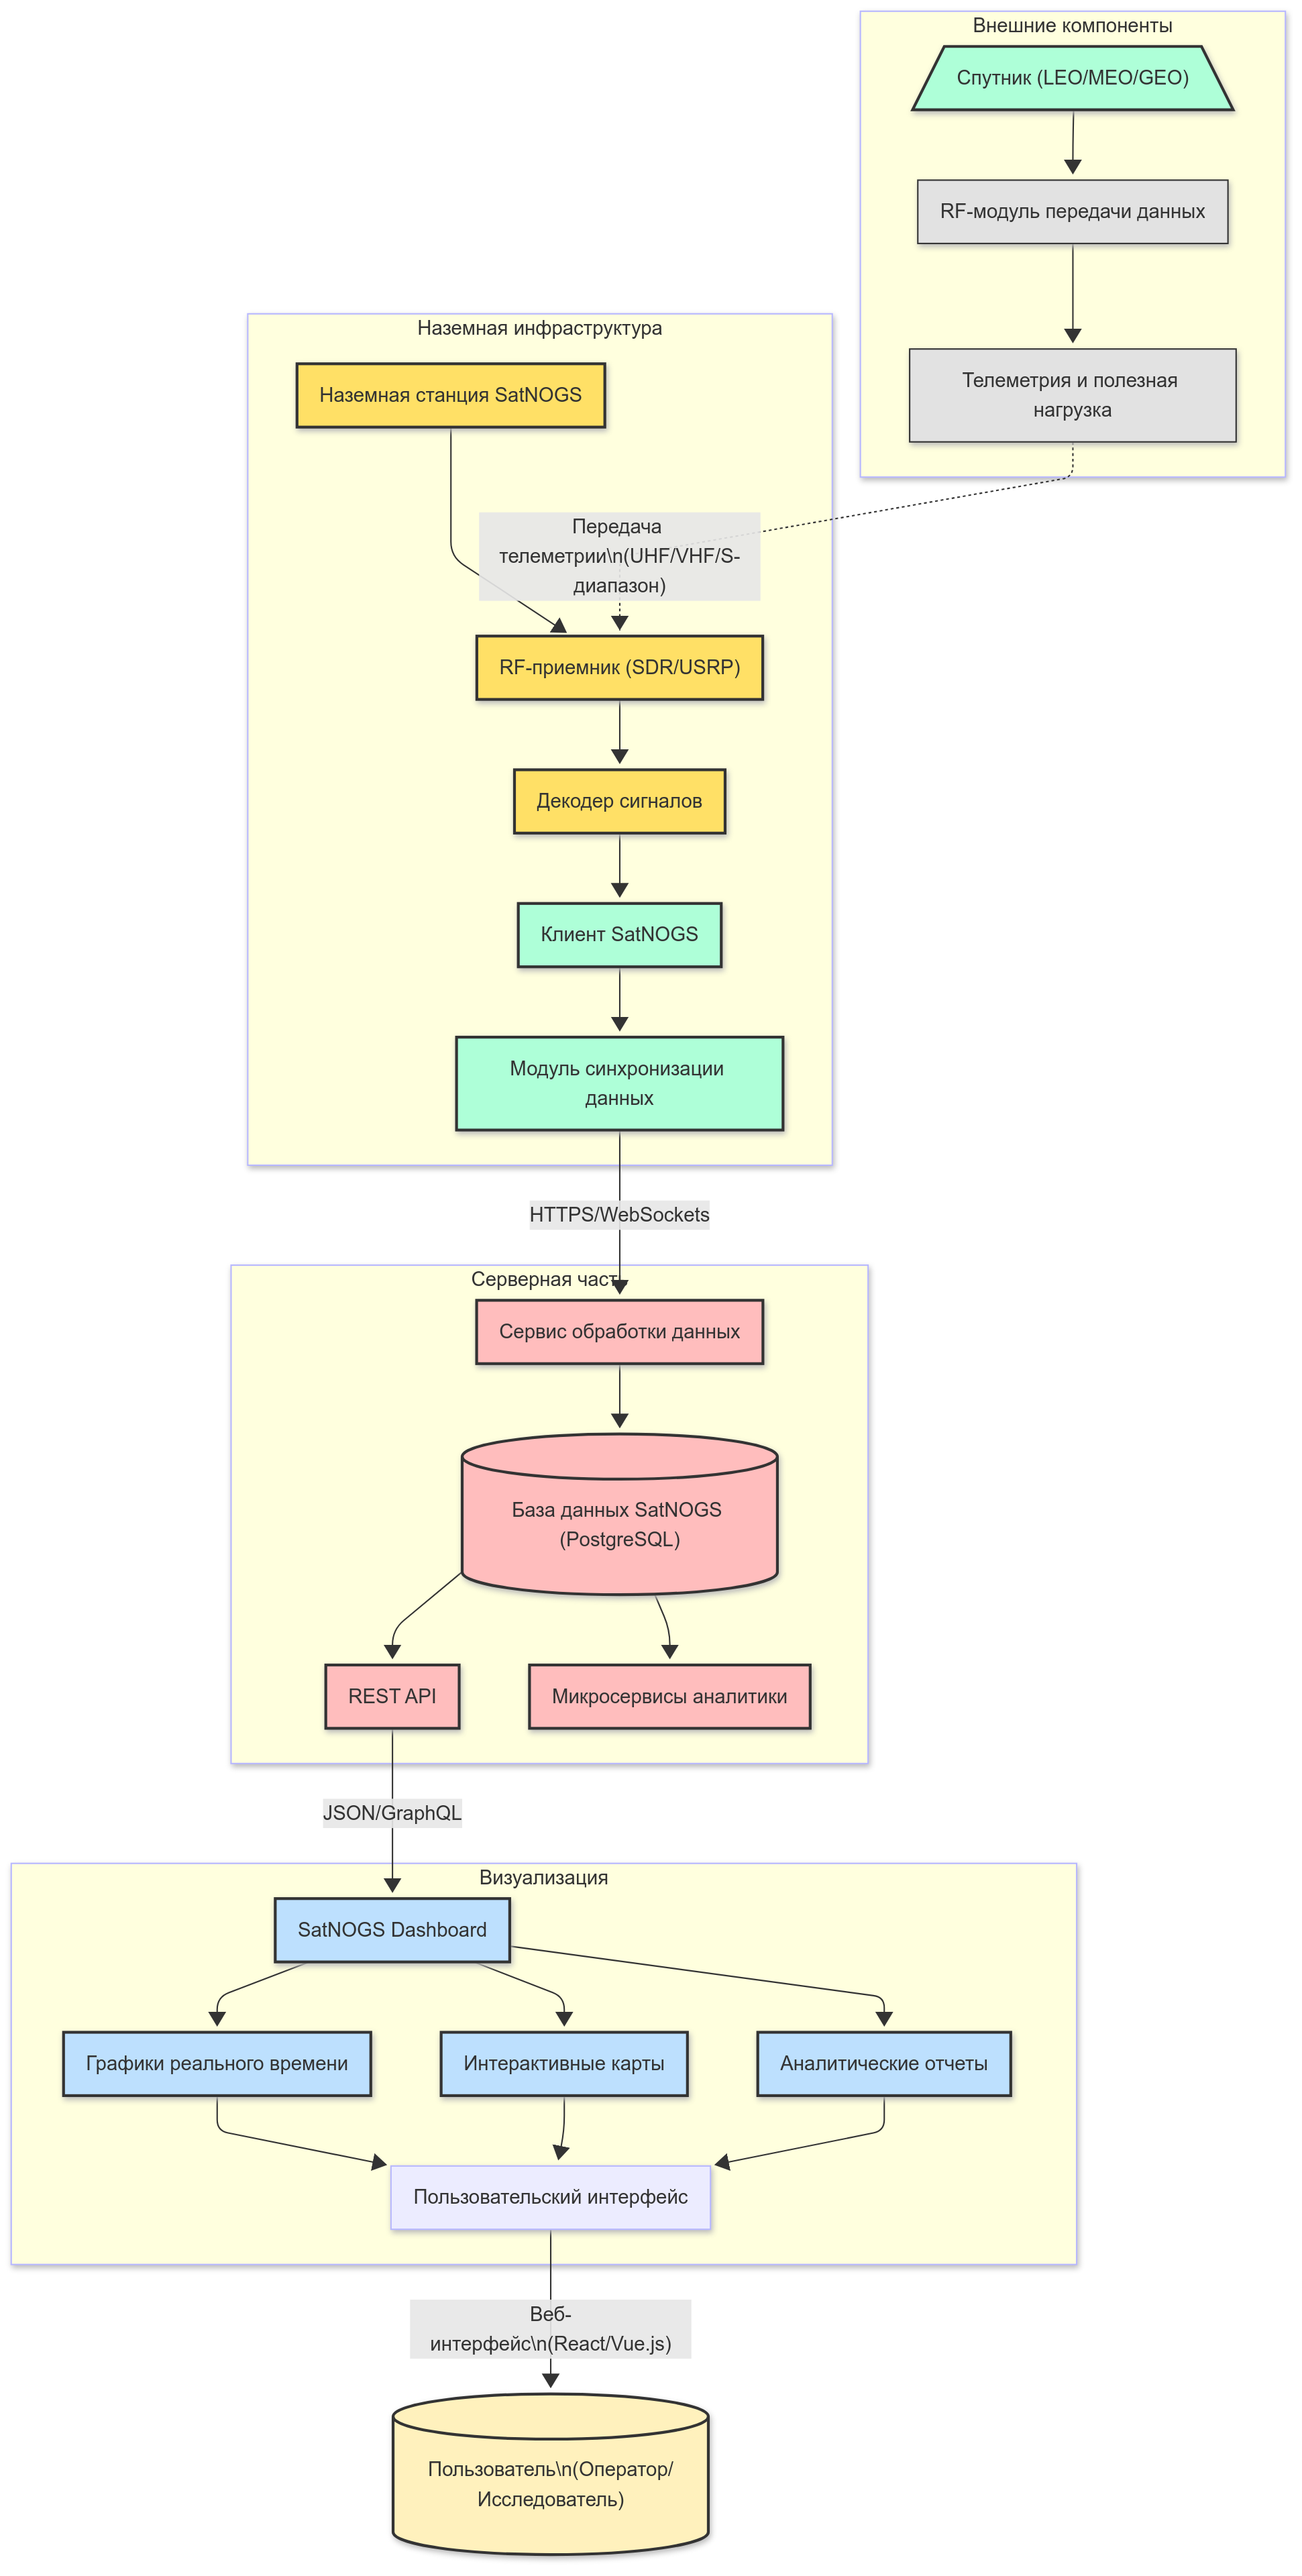
\includegraphics[width=0.7\textwidth]{satnogs_data_flow}
	\caption{Поток данных SatNOGS в Dashboard endpoint}
	\label{fig:satnogs_data_flow}
\end{figure}

\section{SatNOGS Dashboard}

SatNOGS Dashboard представляет собой ключевой компонент в нашей
исследовательской работе, выступая в качестве основного источника данных для
обучения моделей. После детального анализа архитектуры системы было определено
оптимальное место для извлечения данных. Dashboard Grafana в рамках экосистемы
SatNOGS предоставляет уже предобработанные данные, прошедшие фильтрацию и
дедупликацию посредством построения временных рядов. Несмотря на то, что
система содержит информацию только о приблизительно 120 спутниках, этот объем
является достаточным для анализа критических метрик и позволяет существенно
сократить затраты времени и вычислительных ресурсов на обучение, при этом
обеспечивая независимость от инфраструктуры SatNOGS.

Grafana -- это мощная платформа для визуализации и анализа данных, которая
позволяет создавать интерактивные дашборды на основе различных источников
данных \cite{grafana_docs}. Пример такого дашборда можно увидеть на рисунке
\ref{fig:grafana_example}.
Grafana широко используется для мониторинга систем и приложений, предоставляя
пользователям возможность отслеживать ключевые метрики в реальном времени.

\begin{figure}[H]
	\centering
	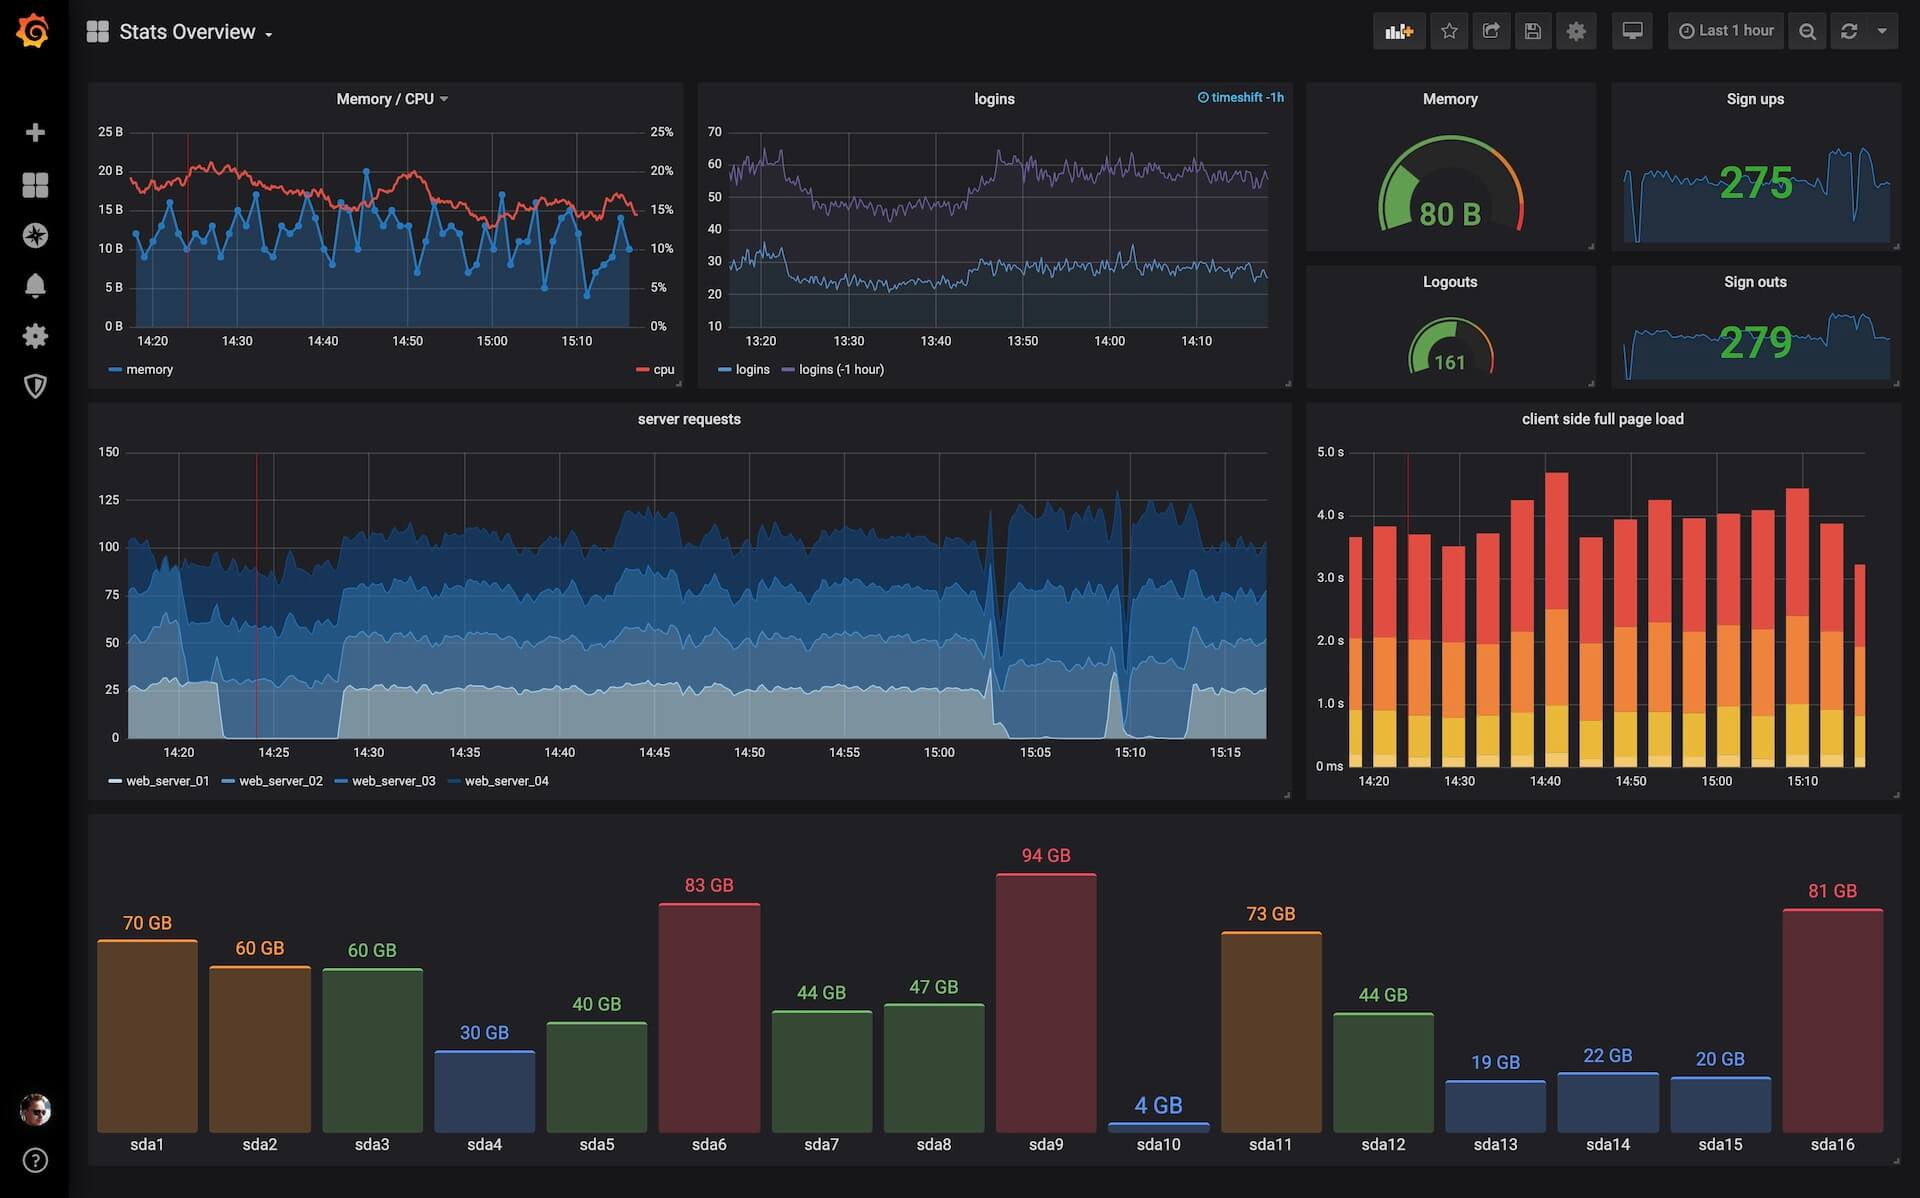
\includegraphics[width=1.0\textwidth]{grafana_example}
	\caption{Пример страницы с данными в Grafana Enterprise}
	\label{fig:grafana_example}
\end{figure}

В контексте SatNOGS Dashboard, Grafana работает с базой данных
\textbf{InfluxDB} \cite{influxdb_docs}, которая предназначена для хранения
временных рядов данных, таких как телеметрия спутников. Данные поступают от
наземных станций, обрабатываются клиентом SatNOGS и сохраняются в InfluxDB.
Затем Grafana использует API для доступа к этим данным и их визуализации на
дашбордах.

Однако стоит отметить, что доступ к API Grafana Dashboard SatNOGS был закрыт,
что ограничивает возможности пользователей в получении данных напрямую. Более
того, Grafana не предоставляет свои услуги пользователям из России и Беларуси в
связи с санциями \cite{grafana_community_post}, что создает дополнительные
сложности для разработчиков и исследователей из этих стран. Это делает Grafana
ненадежной платформой для работы в нашем регионе.

В ответ на эти ограничения нами разрабатывается специализированный парсер для
обхода существующих барьеров и получения необходимых данных. Данный инструмент
будет подробно рассмотрен в последующих разделах работы, поскольку он является
ключевым компонентом для интеграции данных из SatNOGS Dashboard в нашу систему
анализа и визуализации.

Таким образом, несмотря на значительный потенциал Grafana как инструмента
визуализации, текущие ограничения доступа существенно снижают её практическую
ценность для пользователей из определённых регионов, что обуславливает
необходимость разработки альтернативных методов работы с данными.
Схему работы SatNOGS Dashboard можно наблюдать на рисунке
\ref{fig:grafana_infra}.

\begin{figure}[H]
	\centering
	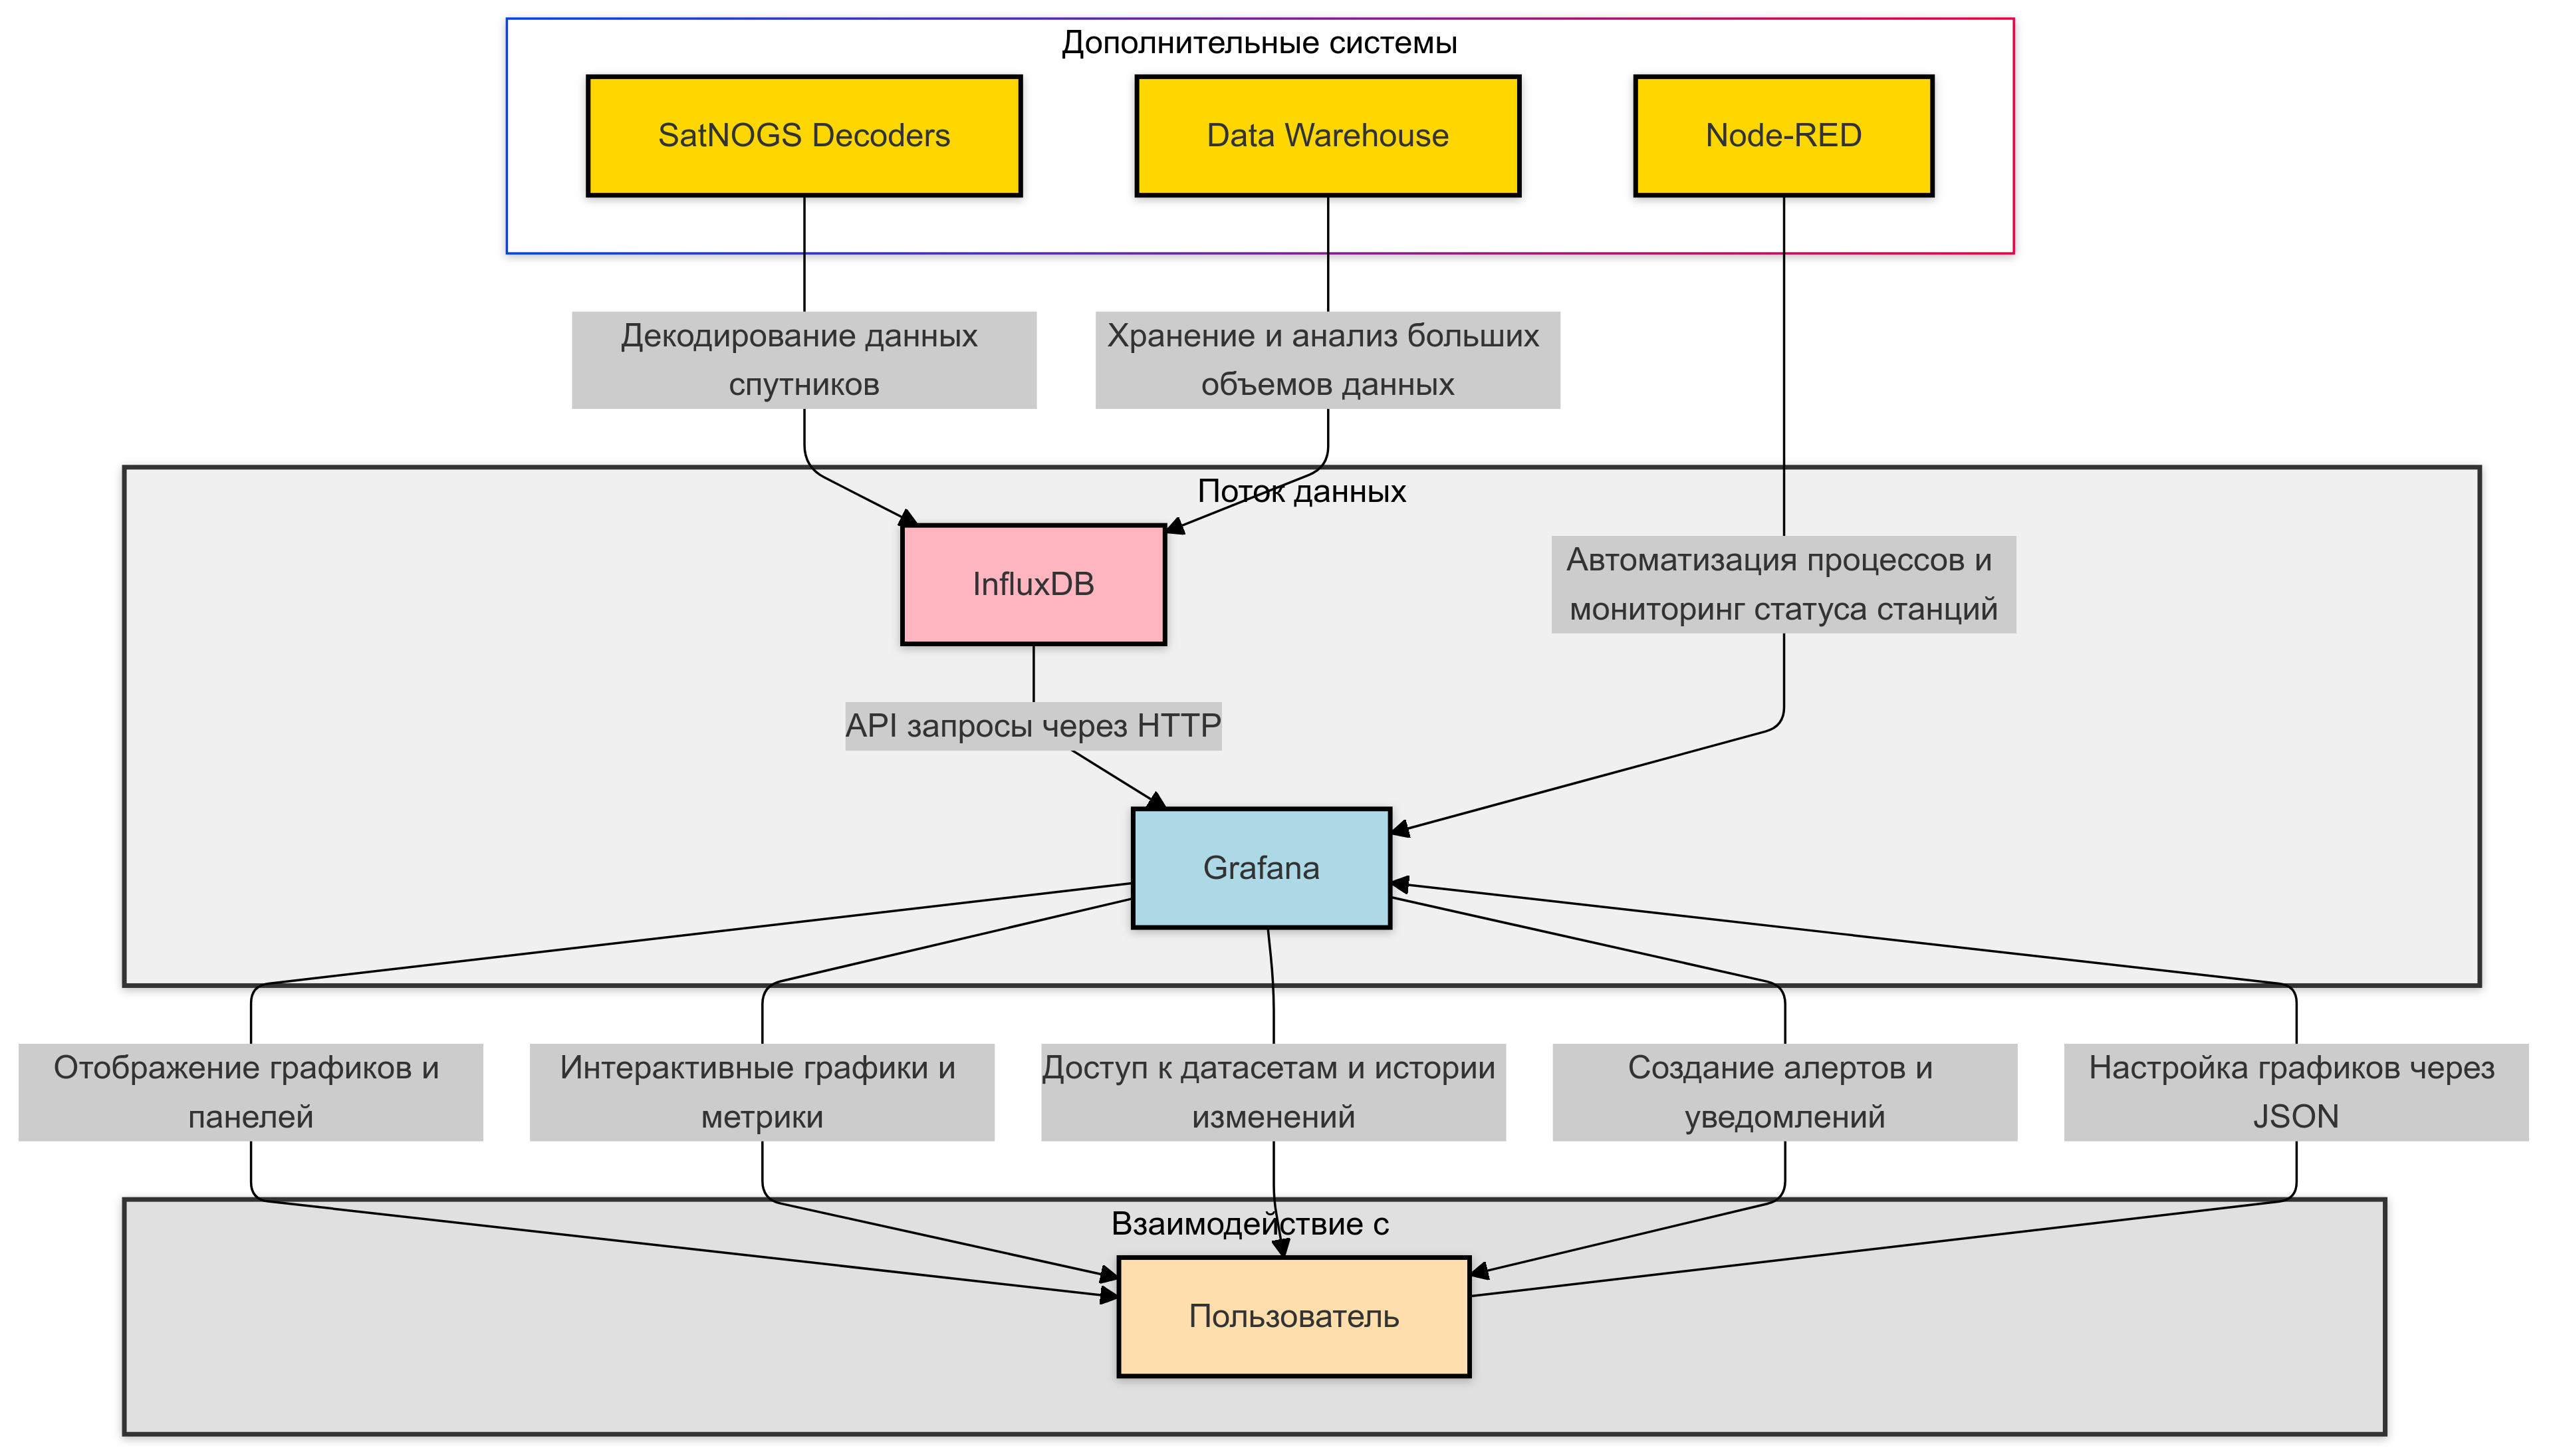
\includegraphics[width=1.0\textwidth]{grafana_infra}
	\caption{Подробное устройство SatNOGS Dashboard}
	\label{fig:grafana_infra}
\end{figure}


Разберем схему архитектуры фронтенд-части системы
\ref{fig:grafana_frontend_structure}
Grafana.
Данная схема иллюстрирует взаимодействие компонентов пользовательского
интерфейса Grafana и потоки данных между ними.

\subsection{Устройство frontend SatNOGS Dashboard}
\begin{figure}[htbp]
	\centering
	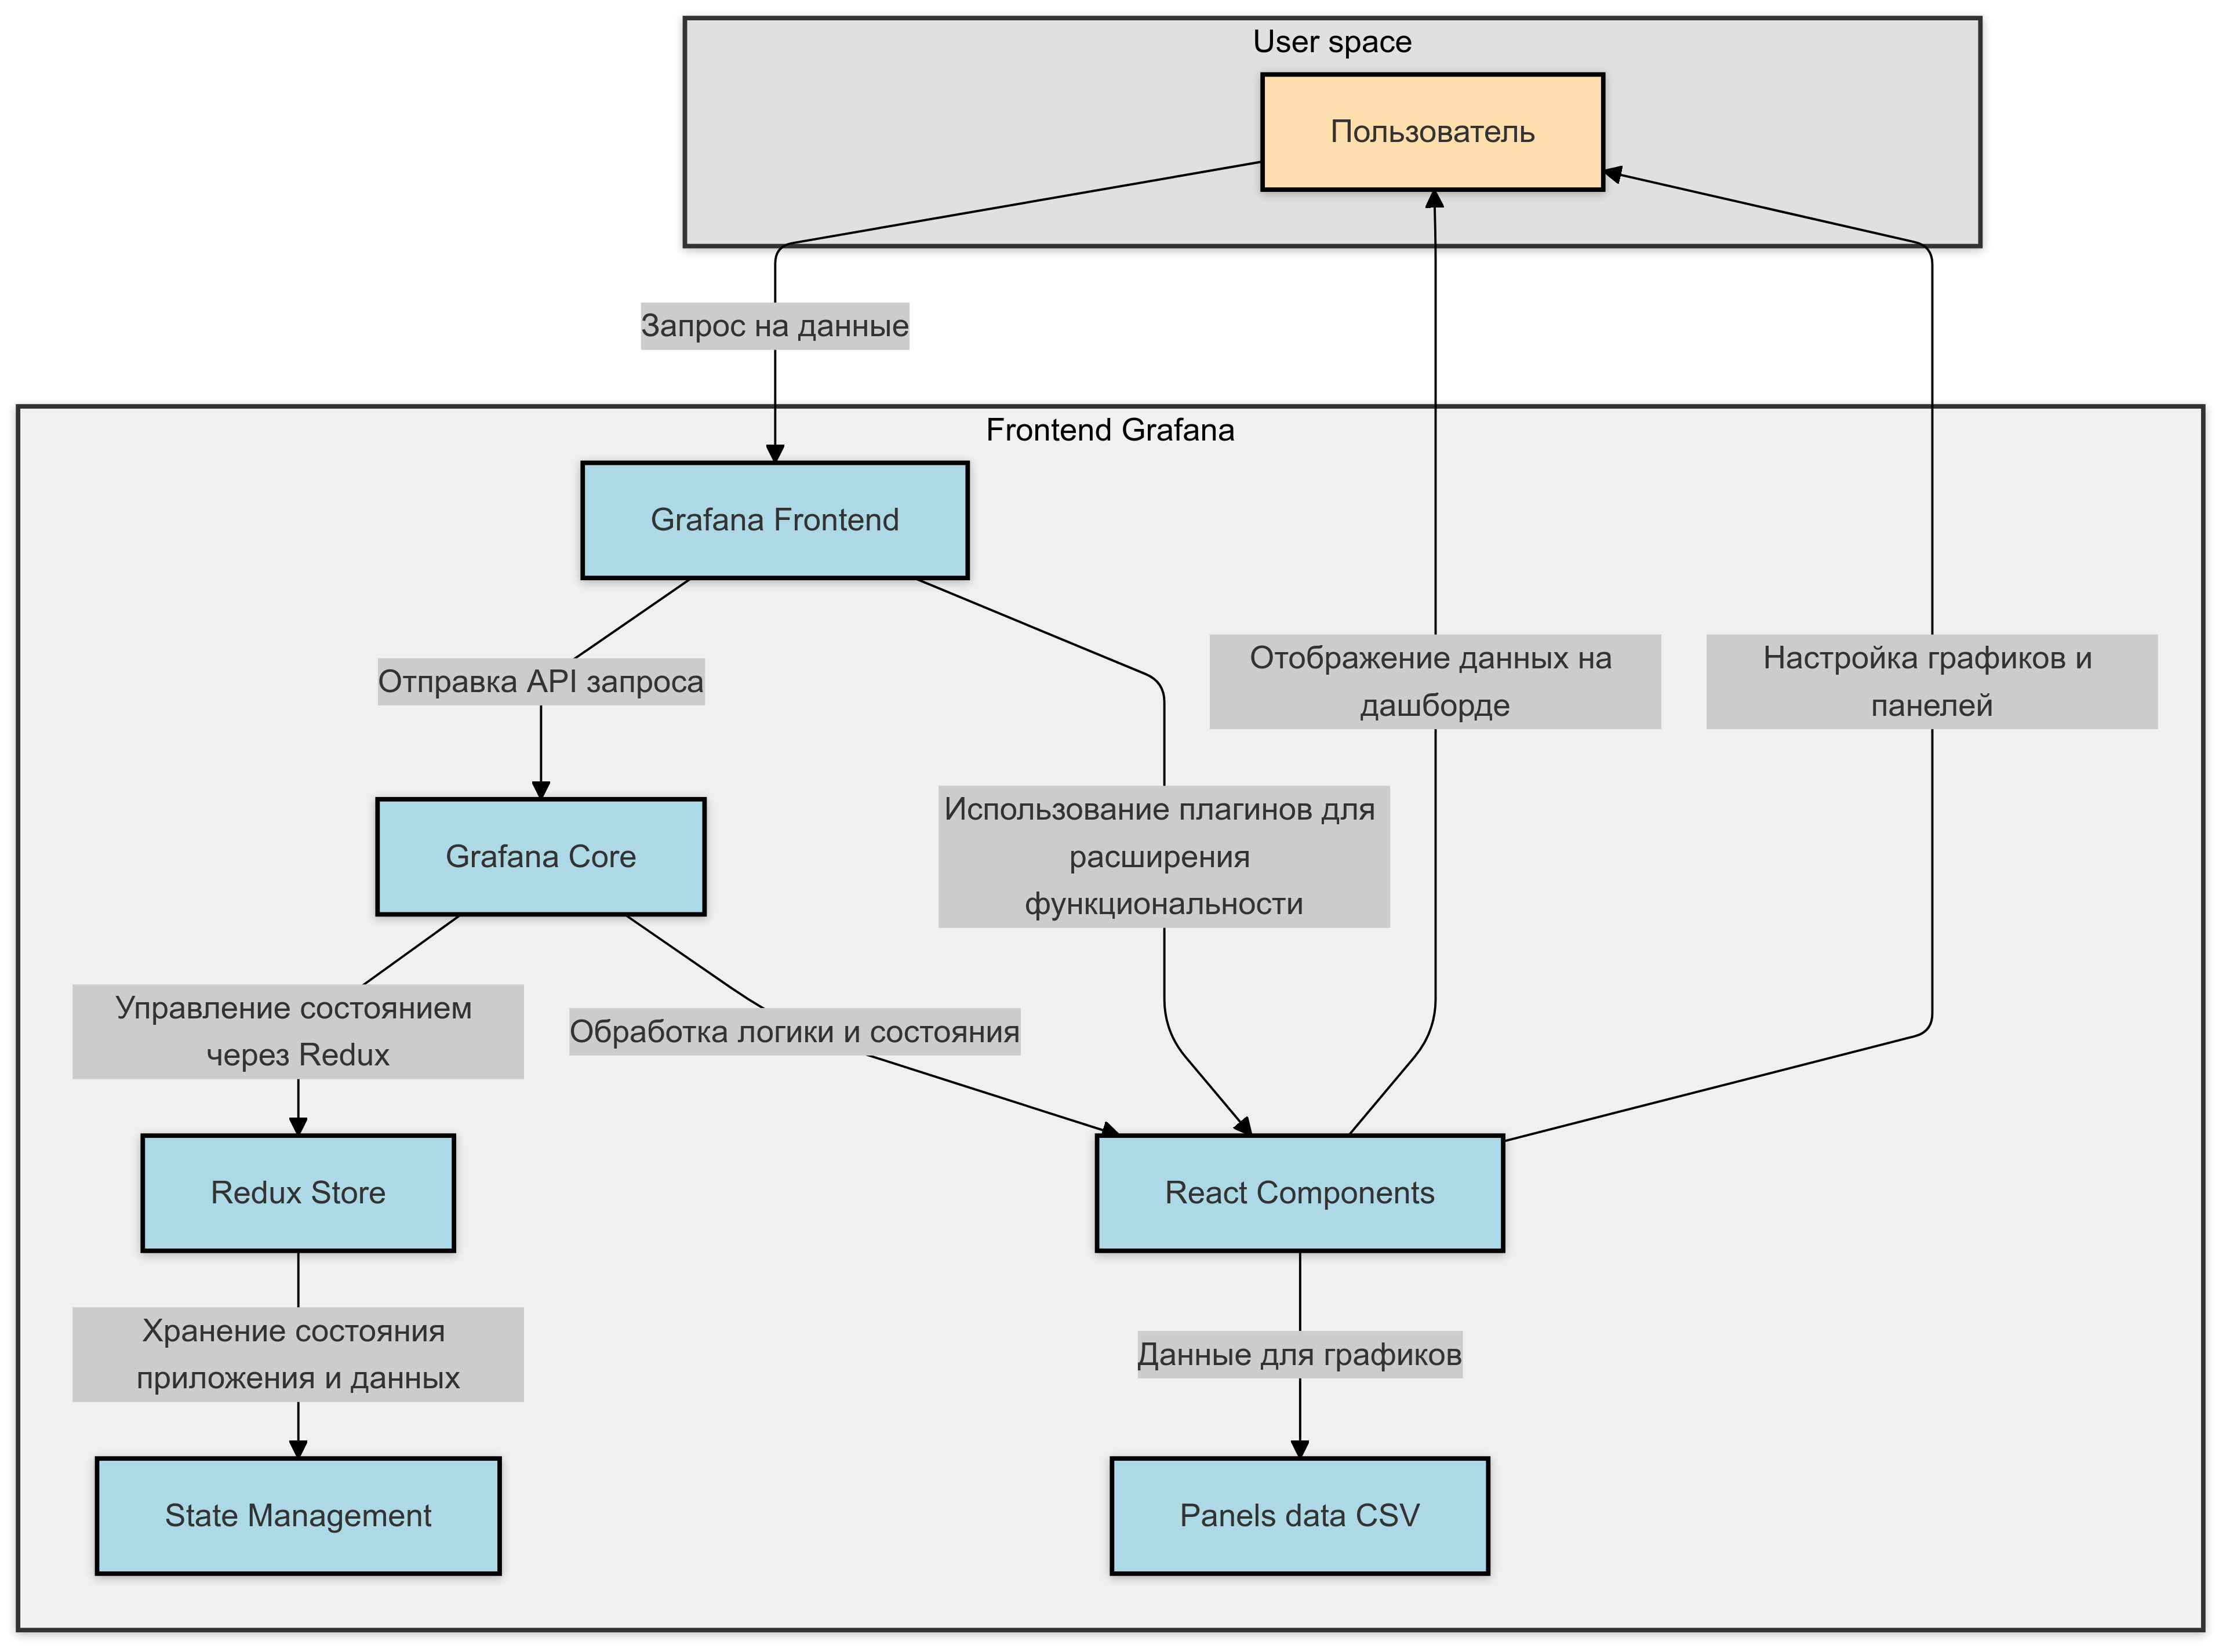
\includegraphics[width=1.0\textwidth]{grafana_frontend_structure}
	\caption{Построение frontend части grafana \cite{react_managing_state}}
	\label{fig:grafana_frontend_structure}
\end{figure}

Архитектура построена по многоуровневому принципу, где пользовательское
пространство (User space) взаимодействует с фронтенд-частью Grafana через
запросы на получение данных. Фронтенд Grafana состоит из нескольких ключевых
компонентов: Grafana Frontend, Grafana Core, Redux Store, State Management,
React Components и Panels data CSV.

Процесс работы системы начинается с запроса пользователя на получение данных,
который обрабатывается компонентом Grafana Frontend. Этот компонент отправляет
API-запросы к Grafana Core, который выполняет обработку логики и состояния.
Grafana Core взаимодействует с Redux Store для управления состоянием приложения
через механизм Redux. State Management отвечает за хранение состояния
приложения и данных.

React Components играют центральную роль в системе, обеспечивая отображение
данных на дашборде, настройку графиков и панелей, а также расширение
функциональности через плагины. Компонент Panels data CSV отвечает за
подготовку данных для графиков.

Для эффективного парсинга данной системы следует сосредоточиться на компоненте
Panels data CSV, который содержит структурированные данные для визуализации, а
также на API-запросах между Grafana Frontend и Grafana Core. Стратегия парсинга
должна учитывать, что данные проходят через несколько уровней обработки,
включая React Components, и хранятся в Redux Store. Понимание этой архитектуры
позволяет определить оптимальные точки извлечения данных и методы обхода
возможных ограничений доступа к API.

\section{Веб скраппер данных}

Представленный скрипт реализует асинхронный механизм извлечения данных из
панелей Grafana Dashboard с использованием библиотеки Playwright для
автоматизации браузера. Рассмотрим его архитектуру и принципы работы в деталях.

\subsection{Архитектура и основные компоненты}

Скрипт построен на основе асинхронной модели программирования Python с
использованием библиотеки asyncio, представляющей собой стандартный
инструментарий для реализации конкурентного выполнения кода. Данная библиотека,
введенная в Python 3.4 и дополненная синтаксисом async/await в Python 3.5,
обеспечивает эффективную обработку множества HTTP-запросов параллельно без
блокировки основной программы.

Архитектура скрипта характеризуется четким разделением основной логики на
функциональные блоки, образующие целостную систему извлечения данных. Блок
управления выполнением осуществляет настройку пулов потоков, дифференцируя
операции ввода-вывода и вычислительные процессы для оптимального использования
системных ресурсов. Механизмы формирования трафика реализуют регулирование
интенсивности запросов, предотвращая возможные блокировки со стороны сервера при
чрезмерной нагрузке.

Существенную роль в функционировании скрипта играет блок разрешения путей,
определяющий расположение JavaScript-файлов, необходимых для взаимодействия с
интерфейсом Grafana. Блок валидации данных обеспечивает проверку и фильтрацию
извлекаемой информации, гарантируя ее соответствие заданным критериям качества.
Завершающим звеном в цепи обработки является блок обработки измерений,
выполняющий анализ и нормализацию единиц измерения в полученных данных.

Центральным элементом всей системы выступает функция grafana\_fetch, которая
инициирует процесс извлечения данных. Данная функция запускает браузер Chromium
посредством библиотеки Playwright и координирует работу всех вышеописанных
компонентов, обеспечивая их согласованное функционирование в рамках единого
цикла событий. Благодаря использованию асинхронного подхода, скрипт способен
эффективно управлять множеством одновременно выполняющихся задач без
существенных затрат ресурсов, что особенно важно при обработке большого
количества HTTP-запросов.

\subsection{Технические особенности реализации}

Скрипт использует ряд технических приемов для повышения эффективности и
надежности, представляющих собой комплексное решение задачи оптимизации
извлечения данных. Асинхронное программирование, реализованное посредством
библиотеки asyncio, обеспечивает эффективную обработку множества запросов
параллельно, что позволяет максимизировать пропускную способность системы при
минимальном использовании вычислительных ресурсов. Данный подход особенно
эффективен при работе с сетевыми операциями, характеризующимися значительными
задержками.

Важным архитектурным решением является разделение операций на IO-bound
(ввод-вывод) и CPU-bound (вычисления) с использованием отдельных пулов потоков.
Такая дифференциация позволяет оптимизировать использование ресурсов системы,
предотвращая блокировку основного потока выполнения при выполнении длительных
операций ввода-вывода и обеспечивая эффективное распределение вычислительной
нагрузки между доступными ядрами процессора.

Механизм регулирования трафика реализован посредством применения случайных
задержек (jitter) между запросами и обработки панелей пакетами с паузами между
ними. Данный подход существенно снижает риск блокировки со стороны сервера,
который может интерпретировать большое количество одновременных запросов как
потенциальную DoS-атаку. Введение стохастического элемента в процесс
формирования запросов делает их паттерн более приближенным к естественному
поведению пользователя.

Комплексная система обработки исключений представляет собой многоуровневый
механизм, обеспечивающий устойчивость скрипта к сбоям отдельных компонентов.
Данная система позволяет продолжать работу даже при возникновении частичных
ошибок, изолируя проблемные участки и предотвращая каскадное распространение
сбоев на весь процесс извлечения данных.

Завершающим элементом оптимизации является применение параллельной обработки
данных с использованием библиотеки pandas. Данный инструментарий обеспечивает
эффективную обработку и трансформацию данных посредством векторизованных
операций, что существенно повышает производительность при работе с большими
объемами информации по сравнению с традиционными итеративными подходами.

\subsection{Практическое применение}

Скрипт предоставляет мощный инструмент для автоматизированного извлечения
данных из Grafana Dashboard, что особенно ценно в контексте ограниченного
доступа к API или при наличии региональных ограничений. Он может быть
интегрирован в более широкие системы анализа данных или мониторинга,
обеспечивая независимость от инфраструктуры Grafana.

Основное преимущество данного подхода заключается в его способности обходить
ограничения стандартного API путем эмуляции взаимодействия пользователя с
интерфейсом. Это позволяет получать данные даже в случаях, когда прямой
доступ к API ограничен или недоступен.

\begin{figure}[H]
	\centering
	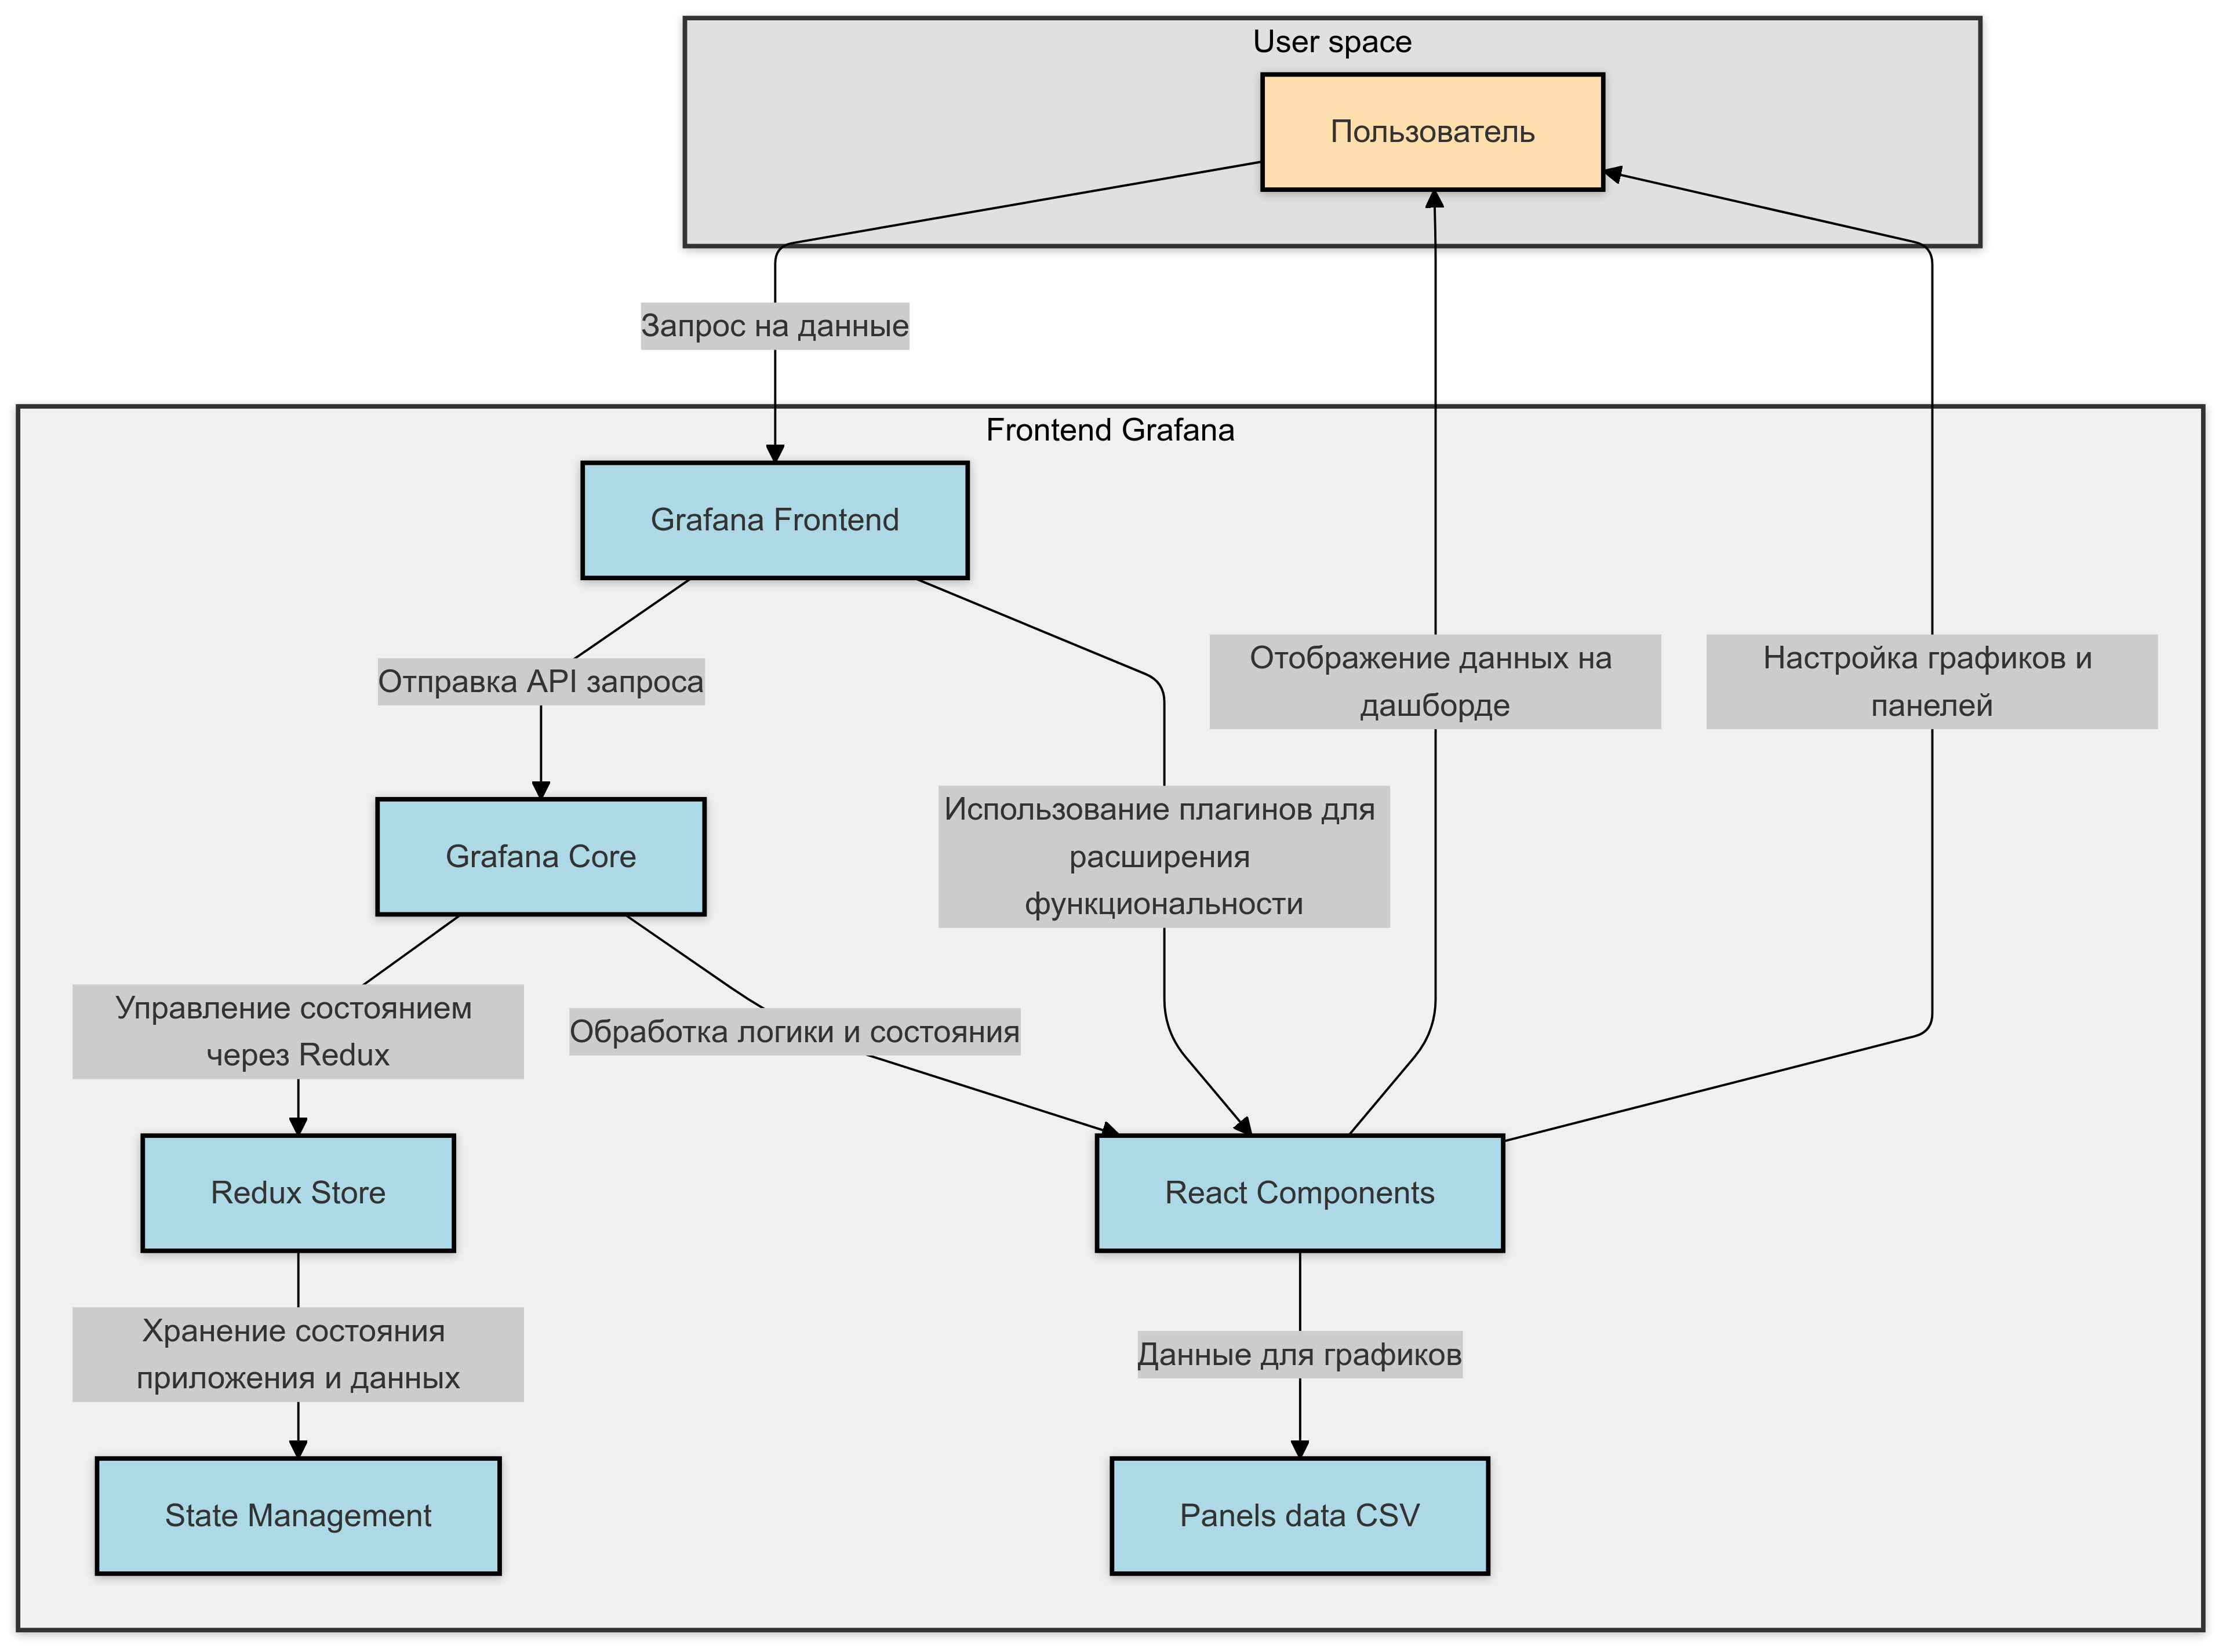
\includegraphics[width=0.9\textwidth]{grafana_frontend_structure}
	\caption{Структура фронтенд-части Grafana, иллюстрирующая компоненты, с которыми взаимодействует скрипт}
	\label{fig:grafana_frontend_structure_advanced}
\end{figure}

Как показано на рисунке \ref{fig:grafana_frontend_structure_advanced}, скрипт
взаимодействует с различными уровнями архитектуры Grafana, включая React
Components и Panels data CSV, что позволяет эффективно извлекать данные, минуя
стандартные ограничения API.

В контексте работы с SatNOGS Dashboard данный скрипт представляет собой
ключевой инструмент для получения телеметрических данных спутников, необходимых
для дальнейшего анализа и обучения моделей. Его применение позволяет преодолеть
ограничения доступа к данным и обеспечить независимость исследовательской
работы от внешней инфраструктуры.


\newpage  
\chapter{Платформа Polaris ML}

Приложение Polaris ML от LibreSpace~\cite{librespace_docs} реализует
инновационный подход к анализу многомерных временных рядов телеметрии
космических аппаратов, основанный на комбинации методов машинного обучения и
теории графов. Система использует модифицированную версию алгоритма
XGBoost~\cite{xgboost_docs} с адаптированной функцией потерь для работы с
нестационарными пространственно-временными данными спутниковых систем.

Архитектура предобработки данных. Первичная обработка сырых телеметрических сигналов включает многоуровневый
конвейер преобразований: очистку от шумов, заполнение пропусков, нормализацию и
другие преобразования, необходимые для корректной работы алгоритмов машинного
обучения.

Обоснование выбора XGBoost. В основе системы Polaris ML лежит алгоритм XGBoost (Extreme Gradient Boosting),
который представляет собой комплексный ансамблевый метод машинного обучения,
базирующийся на принципах градиентного бустинга. При выборе данного алгоритма
решающую роль сыграли его исключительные возможности по обработке данных сложной
структуры. Прежде всего следует отметить способность XGBoost эффективно
анализировать нелинейные зависимости высокой размерности, включающие до 128
взаимосвязанных параметров одновременно. Не менее важным преимуществом является
возможность учета временных задержек между событиями, что позволяет выявлять так
называемые time-lagged correlations, критически важные для прогнозирования
поведения динамических систем. Кроме того, алгоритм демонстрирует высокую
эффективность при работе с иерархическими структурами данных, такими как
вложенные пакеты телеметрии, что существенно расширяет область его практического
применения в сложных технических системах \cite{luppen2021introducing}. Данные
особенности в совокупности обеспечивают Polaris ML значительное преимущество
перед альтернативными решениями при решении задач высокой вычислительной
сложности.

Преимущества ансамблевого подхода XGBoost в контексте спутниковых систем
представляют собой комплекс технических характеристик, обеспечивающих
эффективность данного алгоритма при работе со спутниковыми данными.
Прежде всего следует отметить превосходство XGBoost над нейросетями в задачах с
временными рядами. Согласно проведенным исследованиям, градиентный бустинг
демонстрирует более высокую точность при прогнозировании временных рядов по
сравнению с рекуррентными нейронными сетями, что особенно важно при анализе
телеметрических данных спутников.

Существенным преимуществом является устойчивость к пропускам в телеметрии.
XGBoost способен эффективно работать с данными, содержащими пропуски, без
необходимости предварительной интерполяции отсутствующих значений. Это
критически важно для спутниковых систем, где сбои в передаче данных могут
приводить к неполным наборам информации.

Отсутствие необходимости нормализации данных также является значимым
преимуществом. Алгоритм работает с исходными величинами без предварительной
нормализации, что снижает риск ошибок предобработки для критических систем. Это
упрощает процесс подготовки данных и уменьшает вероятность внесения искажений на
этапе предобработки.

Интерпретируемость модели выгодно отличает XGBoost от нейросетей, представляющих
собой "черный ящик". Алгоритм позволяет анализировать важность признаков и
конкретные решающие правила, что необходимо для сертификации системы управления
спутником. Возможность объяснить принимаемые моделью решения повышает доверие к
системе и упрощает процесс отладки.

Последовательное улучшение через анализ ошибок является фундаментальным
принципом работы XGBoost. Каждое следующее дерево в ансамбле фокусируется на
исправлении ошибок предыдущих, что обеспечивает робастность к шумам в
телеметрических данных. Такой подход позволяет достигать высокой точности даже
при наличии зашумленных данных, характерных для спутниковых систем.

Эффективное использование вычислительных ресурсов делает XGBoost особенно
привлекательным для применения в спутниковых системах с ограниченными
вычислительными возможностями. Модель требует значительно меньше памяти и
процессорного времени по сравнению с глубокими нейронными сетями. Это позволяет
реализовывать сложные алгоритмы анализа данных даже на бортовых компьютерах
спутников с ограниченными ресурсами.

Наконец, встроенная регуляризация в виде механизмов L1 и L2 регуляризации в
XGBoost предотвращает переобучение даже при ограниченном объеме обучающих
данных, что актуально для новых спутниковых платформ. Это особенно важно в
начальных этапах эксплуатации спутниковых систем, когда объем накопленных данных
еще недостаточен для обучения сложных моделей без риска переобучения.

Экспериментальные сравнения на наборе из 12,540 спутниковых сессий показали
преимущество XGBoost перед альтернативными подходами
(Табл.~\ref{tab:ml_comparison})

\begin{table}[H]
        \caption{Сравнение алгоритмов на тестовом наборе телеметрии исходной модели polaris}
	\centering
	\begin{tabular}{|l|c|c|c|}
		\hline
		\textbf{Алгоритм} & \textbf{F1-Score} & \textbf{Время обучения (мин)} & \textbf{Память (GB)} \\
		\hline
		Random Forest     & 0.87              & 45                            & 8.2                  \\
		\hline
		LSTM              & 0.91              & 132                           & 14.7                 \\
		\hline
		XGBoost           & 0.94              & 27                            & 5.1                  \\
		\hline
		CatBoost          & 0.93              & 30                            & 6.0                  \\
		\hline
		GRU               & 0.90              & 110                           & 13.5                 \\
		\hline
		SVM               & 0.85              & 60                            & 7.0                  \\
		\hline
	\end{tabular}
	\label{tab:ml_comparison}
\end{table}

Модификации базового алгоритма XGBoost в платформе PolarisML представляют собой
комплекс усовершенствований, направленных на повышение эффективности обнаружения
аномалий в телеметрических данных космических аппаратов. Базовый алгоритм
XGBoost, реализующий метод Ньютона-Рафсона, был существенно доработан для
решения специфических задач анализа телеметрии спутников.

В первую очередь следует отметить введение временных признаков второго порядка
через механизм скользящих окон. Данный подход позволяет учитывать не только
мгновенные значения параметров, но и их динамику во времени, что критически
важно при анализе поведения бортовых систем космического аппарата.

Другим важным усовершенствованием стала реализация специализированной функции
потерь, учитывающей физические ограничения систем спутника. В отличие от
стандартных функций потерь, применяемых в XGBoost, данная модификация позволяет
интегрировать в процесс обучения модели априорные знания о допустимых режимах
работы бортовой аппаратуры.

Для снижения вероятности ложных срабатываний был разработан каскадный подход с
поэтапным уточнением предсказаний. Данный метод предполагает последовательное
применение нескольких моделей с возрастающей сложностью, что обеспечивает
фильтрацию потенциальных аномалий и минимизацию ложноположительных результатов.

Завершающим элементом модификаций стало применение техники стекинга для
объединения предсказаний моделей различной глубины. Данный подход существенно
повышает стабильность работы системы при обнаружении редких аномалий, которые
могут быть пропущены отдельными моделями.

Особую ценность представляет возможность анализа структуры построенных деревьев
решений для выявления неочевидных физических зависимостей в работе бортовых
систем и последующего совершенствования инженерных моделей спутника.


\section{Алгоритм XGBoost}

Алгоритм XGBoost представляет собой мощный метод построения ансамблей решающих
деревьев, основанный на принципе градиентного бустинга. Рассмотрим его
математическую формализацию.

Инициализация модели начинается с определения базового предиктора $F_0(x)$,
который минимизирует функцию потерь на обучающей выборке:

\[F_0(x) = \arg \min_{\gamma} \sum_{i=1}^n L(y_i, \gamma)\]

Далее следует итеративный процесс построения ансамбля. На каждой итерации $m$
вычисляются градиенты и значения функции потерь для каждого объекта:

\begin{gather*}
	g_i = \frac{\partial L(y_i, F_{m-1}(x_i))}{\partial F_{m-1}(x_i)}\\
	h_i = \frac{\partial^2 L(y_i, F_{m-1}(x_i))}{\partial F_{m-1}(x_i)^2}
\end{gather*}

Затем строится дерево решений $f_m(x)$, оптимизирующее следующую целевую функцию:

\[\mathcal{L}^{(m)} = \sum_{i=1}^n \left[ g_i f_m(x_i) + \frac{1}{2} h_i f_m^2(x_i) \right] + \Omega(f_m)\]

где $\Omega(f_m)$ - функция регуляризации, контролирующая сложность дерева. Эта
формулировка учитывает как точность предсказаний, так и структурную сложность
модели, что является ключевым аспектом XGBoost.

Модель обновляется аддитивно:

\[F_m(x) = F_{m-1}(x) + \alpha_m f_m(x)\]

где $\alpha_m$ - коэффициент обучения, определяющий вклад нового дерева.

Процесс повторяется до достижения заданного числа итераций $M$. Финальное
предсказание для нового объекта $x$ формируется как сумма предсказаний всех
деревьев:

\[\hat{y} = F_M(x) = \sum_{m=1}^M \alpha_m f_m(x)\]

Этот алгоритм эффективно комбинирует множество слабых предикторов в сильную
модель, способную улавливать сложные нелинейные зависимости в данных.
Регуляризация и оптимизация второго порядка позволяют XGBoost достигать высокой
точности при сохранении вычислительной эффективности, что делает его одним из
наиболее востребованных алгоритмов в современном машинном обучении.

\section{Процесс анализа телеметрических данных}

Анализ телеметрических данных космических аппаратов представляет собой
многоэтапный процесс, требующий строгой формализации. Рассмотрим ключевые
аспекты методологии, обеспечивающей эффективное выявление аномалий и анализ
взаимосвязей параметров.

Начальный этап предполагает сегментацию временного ряда телеметрии на фреймы
фиксированной длительности $T$, определяемой характерным временем наблюдаемых
процессов. Для непрерывного потока данных $\{x_t\}_{t=1}^N$ это осуществляется
через оконную функцию:

\[
	X_k = \{x_{k \cdot T + 1}, x_{k \cdot T + 2}, \ldots, x_{(k+1) \cdot T}\}, \quad k \in \{0, 1, \ldots, \lfloor N/T \rfloor - 1\}
\]

где $X_k$ - k-ый фрейм данных. Альтернативный подход использует адаптивное
разбиение по событиям $\{E_i\}_{i=1}^M$, определяя границы фреймов условиями
$\|x_t - x_{t_{\text{start}}}\| > \Delta_{\text{threshold}}$.

Из каждого фрейма извлекается вектор признаков $\phi(X_k) \in \mathbb{R}^d$, включающий:

\[
	\phi(X_k) = \left[\mu(X_k), \sigma^2(X_k), \min(X_k), \max(X_k), \sum_{t=1}^T x_t \cdot e^{-j2\pi ft/T}\right]
\]

\noindent где:
\begin{itemize}
	\item $\phi(X_k)$ -- результирующий вектор признаков для $k$-го окна сигнала $X_k$;
	\item $\mu(X_k)$ -- среднее значение амплитуды сигнала в окне $X_k$, характеризующее общий уровень сигнала;
	\item $\sigma^2(X_k)$ -- дисперсия сигнала в окне $X_k$, отражающая меру разброса значений относительно среднего;
	\item $\min(X_k)$ -- минимальное значение сигнала в окне $X_k$, определяющее нижнюю границу амплитуды;
	\item $\max(X_k)$ -- максимальное значение сигнала в окне $X_k$, определяющее верхнюю границу амплитуды;
	\item $\sum_{t=1}^T x_t \cdot e^{-j2\pi ft/T}$ -- коэффициент дискретного преобразования Фурье для частоты $f$, где $x_t$ -- отсчёты сигнала, $T$ -- количество отсчётов в окне, $j$ -- мнимая единица, позволяющий выделить частотные характеристики анализируемого сигнала.
\end{itemize}

Данный вектор признаков комбинирует статистические характеристики сигнала во
временной области с его спектральными свойствами, обеспечивая комплексное
представление для последующего анализа.

Обучение модели XGBoost осуществляется на множестве $\{\phi(X_k),
	y_k\}_{k=1}^K$, где $y_k$ - целевой параметр телеметрии. Целевая функция
оптимизации принимает вид:

\[
	\mathcal{L} = \sum_{k=1}^K \left( y_k - F(\phi(X_k)) \right)^2 + \lambda \sum_{m=1}^M \alpha_m^2 + \gamma \sum_{j=1}^J T_j
\]

\noindent где:
\begin{itemize}
	\item $\mathcal{L}$ -- целевая функция потерь модели, минимизируемая в процессе обучения;
	\item $\sum_{k=1}^K \left( y_k - F(\phi(X_k)) \right)^2$ -- сумма квадратов ошибок модели на всех $K$ обучающих примерах, где $y_k$ -- истинное значение целевой переменной, а $F(\phi(X_k))$ -- предсказание модели на основе вектора признаков $\phi(X_k)$;
	\item $\lambda \sum_{m=1}^M \alpha_m^2$ -- член регуляризации L2-нормы для весов деревьев $\alpha_m$, где $\lambda$ -- коэффициент регуляризации, контролирующий силу штрафа, а $M$ -- общее количество деревьев в ансамбле;
	\item $\gamma \sum_{j=1}^J T_j$ -- дополнительный член регуляризации, накладывающий штраф на сложность модели через суммарное количество листьев $T_j$ в каждом дереве $j$, где $\gamma$ -- соответствующий коэффициент регуляризации, а $J$ -- количество деревьев с учетом их структуры.
\end{itemize}

Данная функция потерь направлена на достижение оптимального баланса между
точностью предсказаний модели и её сложностью, предотвращая переобучение путём
контроля как весов отдельных деревьев, так и их структурной сложности.

Выявление аномалий основано на анализе остатков $\epsilon_k = y_k - \hat{y}_k$. Для каждого параметра определяются:

1. Пороговый критерий: $\|\epsilon_k\| > 3\sigma_\epsilon$
2. Z-нормализация: $z_k = \frac{\epsilon_k - \mu_\epsilon}{\sigma_\epsilon}$
3. Статистика Граббса: $G = \frac{\max |\epsilon_k|}{\sigma_\epsilon}$

где $\mu_\epsilon$ и $\sigma_\epsilon$ - среднее и стандартное отклонение остатков на обучающей выборке.

Ключевым аспектом анализа становится построение графов связности $G=(V,E)$ на
основе матрицы взаимной информации:

\[
	I(X^{(i)}, X^{(j)}) = \sum_{x \in X^{(i)}} \sum_{y \in X^{(j)}} p(x,y) \log \frac{p(x,y)}{p(x)p(y)}
\]

Вершины $v \in V$ соответствуют параметрам телеметрии, рёбра $e \in E$
взвешиваются значениями $I(X^{(i)}, X^{(j)})$. Топология графа визуализирует
скрытые взаимозависимости, позволяя выявлять каскадные эффекты в бортовых
системах.

\section{Проблемы исходной модели и их решение}

В платформе Polaris ML используется стандартный упрощенный вариант XGBoost, который ограничивается малым количеством оптимизируемых гиперпараметров. Такой подход позволяет упростить процесс настройки модели и сохранить вычислительную эффективность, что особенно важно в контексте обработки больших потоков телеметрических данных в реальном времени. Тем не менее, данный метод имеет свои ограничения.

Алгоритм XGBoost в Polaris ML конфигурируется через сеточный поиск гиперпараметров (grid search), который является одной из самых простых, но далеко не самых эффективных стратегий оптимизации. Сеточный поиск представляет собой перебор фиксированного набора параметров по заранее определенной сетке, что может быть вычислительно затратным, особенно при увеличении размерности гиперпараметров. Кроме того, он не учитывает возможные взаимодействия между параметрами и не адаптируется в зависимости от текущих результатов оптимизации. Это может привести к пропуску оптимальных значений параметров или необходимости значительного увеличения вычислительных ресурсов для достижения удовлетворительных результатов.

В последние годы появились более совершенные методы оптимизации гиперпараметров \cite{grid_search_tuning}, такие как Halving Grid Search, Random Search и Bayesian Optimization. Halving Grid Search, например, использует итеративное уменьшение пространства поиска, концентрируясь на наиболее перспективных комбинациях параметров. Это позволяет существенно сократить время подбора, особенно при использовании перекрестной валидации (cross-validation), которая увеличивает точность оценки моделей, но также повышает вычислительную нагрузку.

\section{Новый формат входных данных}

Существенные изменения коснулись и самих данных \ref{fig:polaris_data_flow}. Теперь используется увеличенный объем входных данных, что способствует созданию более точных и устойчивых моделей. В дополнение к этому появилась возможность добавлять собственные данные о солнечной активности, оформленные в формате polars/pandas DataFrame. Ранее такая возможность была доступна только для спутниковых данных, и пользователям приходилось самостоятельно декодировать их перед использованием. Устранение этапа декодирования кадров стало важным шагом вперед: теперь данные загружаются напрямую из SatNOGS Grafana Dashboard, что существенно упрощает их обработку. Прямое формирование DataFrame избавляет пользователей от необходимости выполнения промежуточных операций, таких как обработка сетевых потоков или декодирование.

\begin{figure}[H]
	\centering
	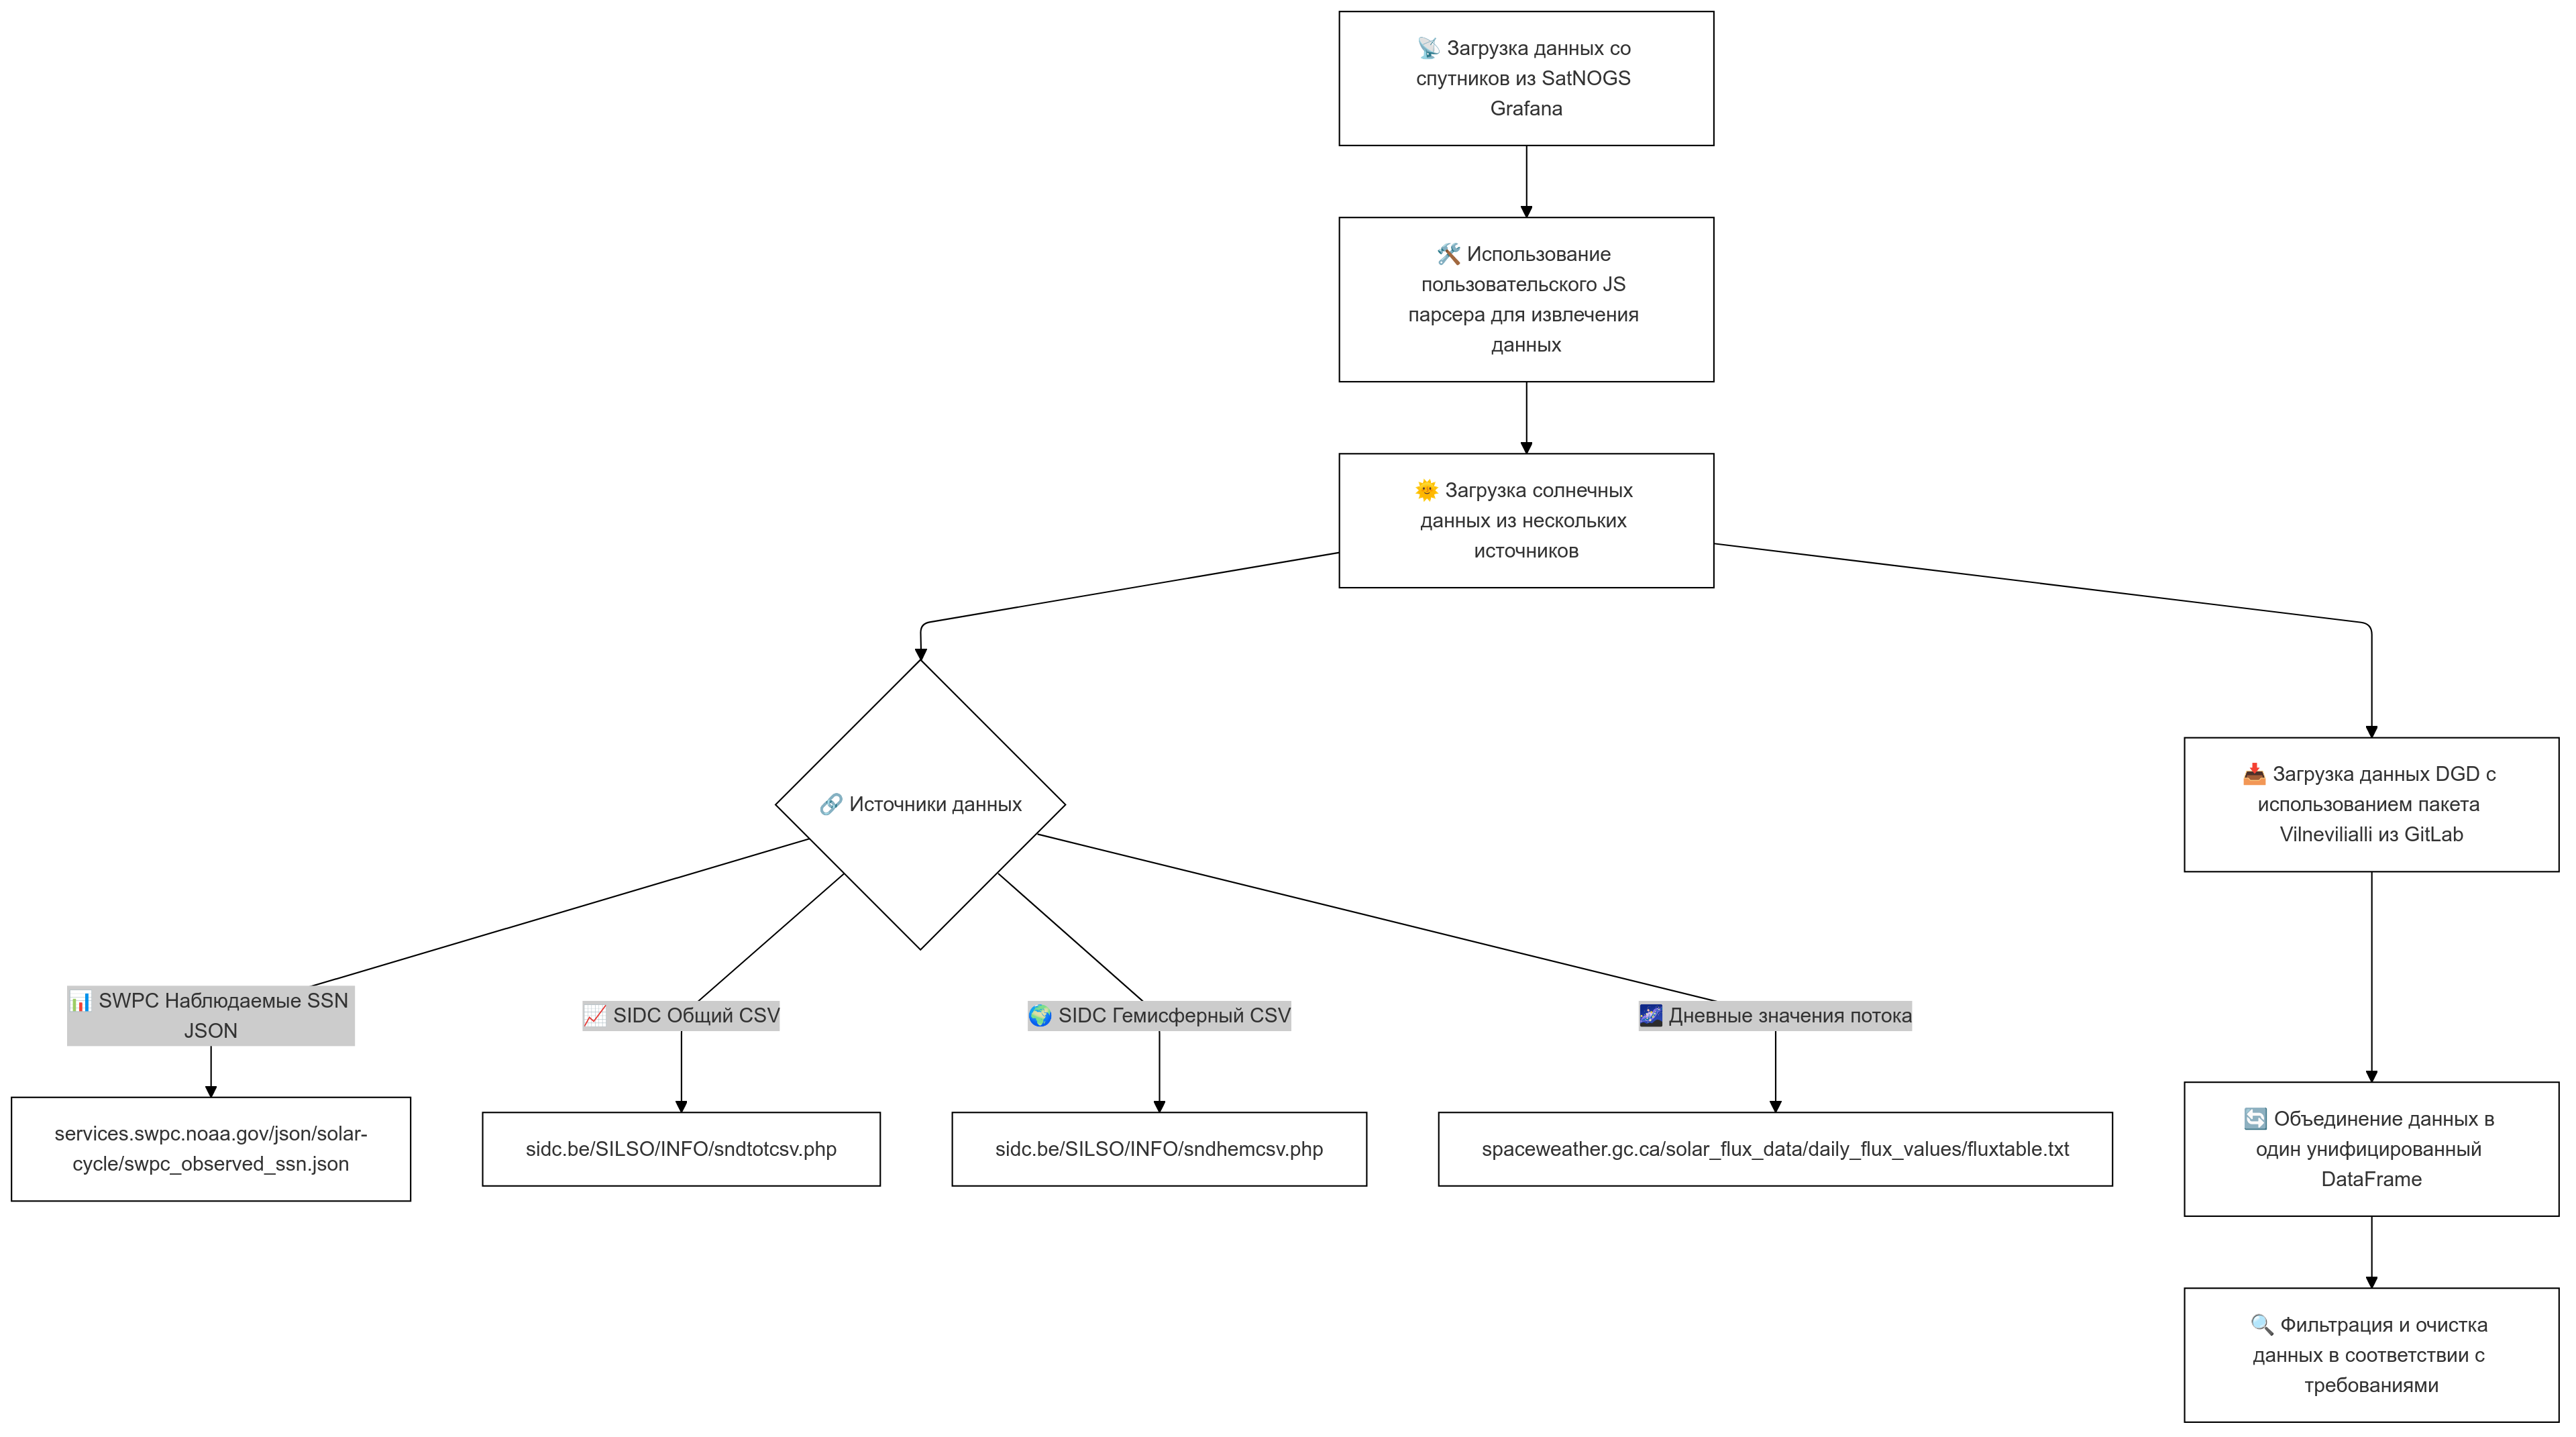
\includegraphics[width=1.0\textwidth]{polaris_data_flow}
	\caption{Измененный входной поток данных для polaris 2.0}
	\label{fig:polaris_data_flow}
\end{figure}

\section{Новый формат графа связности}

Для визуализации данных и анализа их взаимосвязей было принято решение о переносе построения графов на внешнюю библиотеку pyecharts \cite{pyecharts_docs}. Это изменение не только устранило необходимость взаимодействия с Node.js-проектами, но и значительно упростило создание графиков и визуализаций, которые теперь могут быть интегрированы в отчетность и презентации без лишних трудозатрат. Кроме того, интеграция с библиотекой pyecharts обеспечила гибкость в настройке визуализаций и расширила возможности по взаимодействию с интерактивными элементами.

Для управления процессами обучения и экспериментов внедрен mlflow \cite{mlflow_docs}, который позволил стандартизировать ведение отчетности. Теперь в отчетный журнал можно автоматически сохранять артефакты обучения, такие как модели, параметры, метрики и визуализации. Это упрощает анализ и повторное использование ранее выполненных экспериментов. Локально развернутый MLflow UI-сервер позволяет интерактивно сравнивать различные модели с различными гиперпараметрами. Это делает процесс подбора параметров прозрачным и управляемым, особенно при использовании новых возможностей для оптимизации до 30 параметров XGBoost.

В числе таких параметров — $gamma$, $max\_depth$, $min\_child\_weight$, $subsample$ и многие другие. Расширенный набор конфигураций позволяет детально подстраивать поведение модели под конкретные задачи. Переход к работе с увеличенным количеством гиперпараметров сделал платформу более гибкой, а процессы обучения — более детализированными.

Еще одним важным улучшением стало перенесение данных в память GPU с оптимальной упаковкой для ускоренного доступа. Это изменение дало значительный прирост в скорости обучения моделей за счет устранения узких мест, связанных с задержками при чтении и записи данных в оперативной памяти. Теперь платформе доступны преимущества параллельных вычислений, которые обеспечивают современные графические процессоры.

В целом, сделан упор на удобство MLOps и упрощение конфигурирования сети (см. рисунок \ref{fig:polaris_core}). Это включает в себя автоматизацию ряда рутинных процессов, связанных с подготовкой данных, настройкой экспериментов и ведением отчетности. Эти изменения обеспечивают не только повышение производительности, но и улучшение пользовательского опыта для инженеров, работающих с Polaris ML. Платформа становится не просто инструментом для анализа телеметрии, но и полноценной экосистемой для управления данными, экспериментами и визуализацией результатов.

\begin{figure}[H]
	\centering
	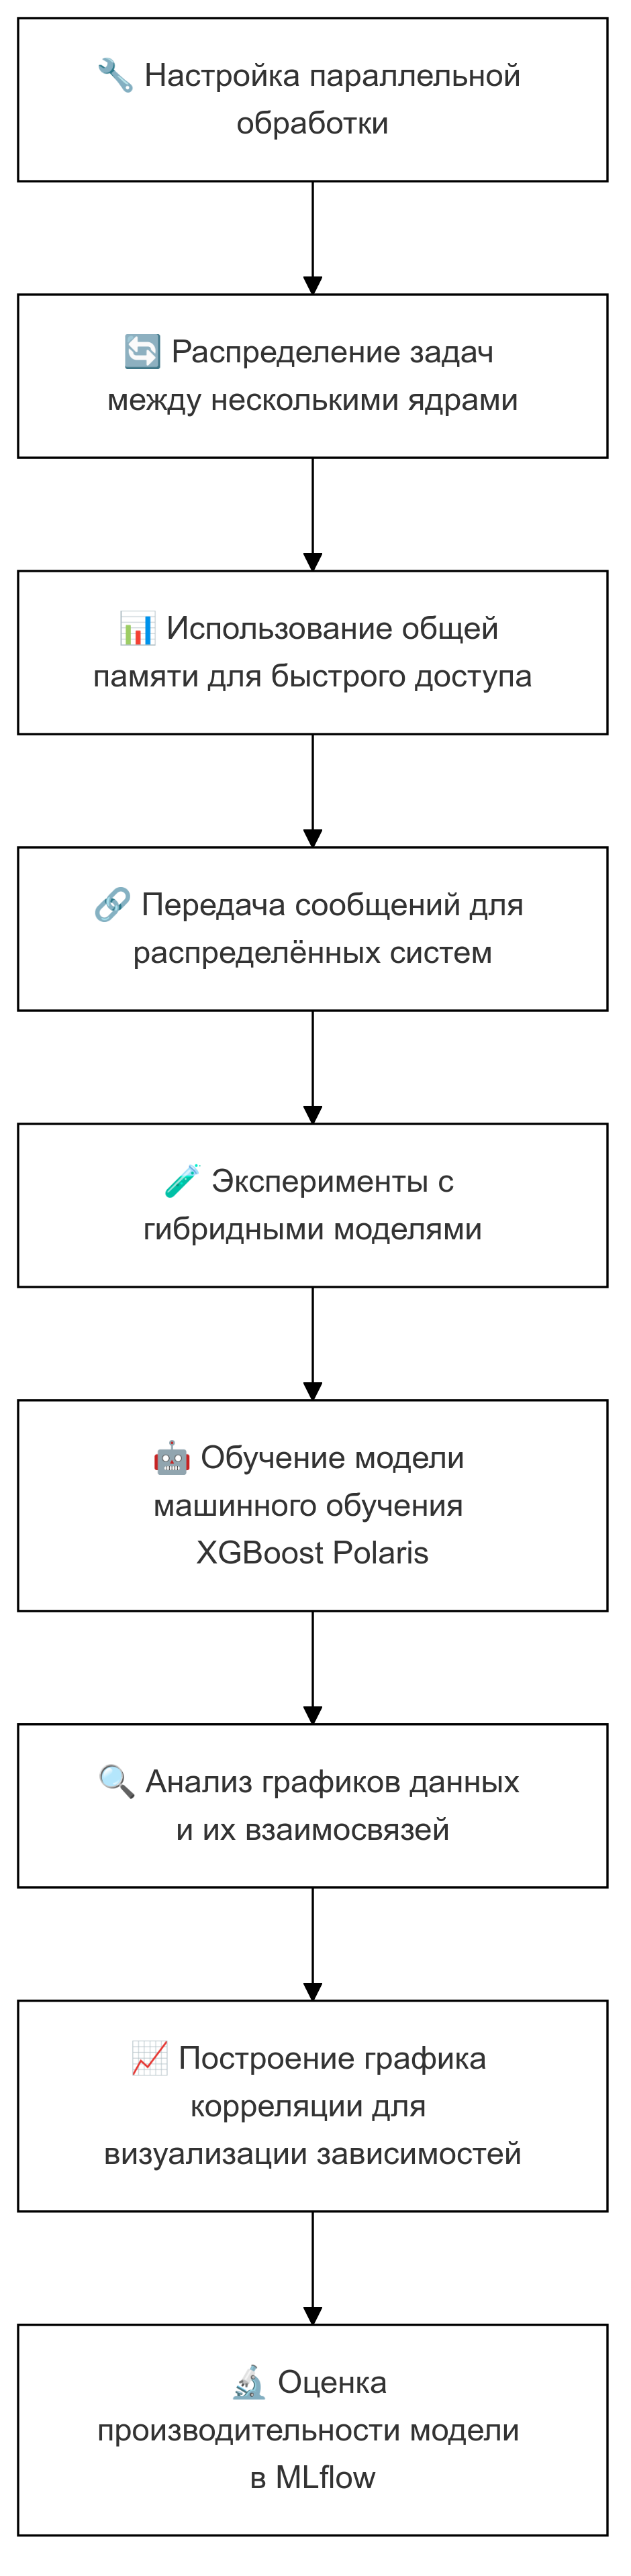
\includegraphics[width=0.34\textwidth]{polaris_core}
	\caption{Ядро polaris 2.0}
	\label{fig:polaris_core}
\end{figure}

В данной таблице представлены основные конфигурируемые и grid-оптимизируемые параметры модели XGBoost \cite{xgboost_parameters_docs}, их описание и значения по умолчанию. Параметры разделены на три категории: общие параметры, параметры бустера и параметры задачи.

\begin{longtable}{|p{4cm}|p{6cm}|p{6cm}|}
	\caption{Параметры XGBoost и их влияние}\label{tab:xgboost_params}                                                                                                                  \\

	\hline
	\textbf{Параметр}             & \textbf{Описание}                                         & \textbf{Влияние}                                                                        \\
	\hline
	\endfirsthead

	\multicolumn{3}{c}%
	{\tablename\ \thetable\ -- \textit{Продолжение}}                                                                                                                                    \\
	\hline
	\textbf{Параметр}             & \textbf{Описание}                                         & \textbf{Влияние}                                                                        \\
	\hline
	\endhead

	\hline \multicolumn{3}{|r|}{\textit{Продолжение на следующей странице}}                                                                                                             \\ \hline
	\endfoot

	\hline
	\endlastfoot

	\texttt{eta (learning\_rate)} & Скорость обучения, регулирует вес новых деревьев          & Слишком низкое значение может привести к недообучению, слишком высокое — к переобучению \\
	\hline
	\texttt{gamma}                & Минимальный прирост в качестве для разбиения узла         & Увеличение значения приводит к более простой модели                                     \\
	\hline
	\texttt{max\_depth}           & Максимальная глубина деревьев                             & Большее значение увеличивает мощность модели, но повышает риск переобучения             \\
	\hline
	\texttt{subsample}            & Доля данных, используемая для обучения каждого дерева     & Снижает переобучение, но может ухудшить точность модели                                 \\
	\hline
	\texttt{colsample\_bytree}    & Доля признаков, используемых для обучения каждого дерева  & Уменьшение значения предотвращает переобучение                                          \\
	\hline
	\texttt{lambda (reg\_lambda)} & L2-регуляризация на веса                                  & Увеличение значения уменьшает переобучение                                              \\
	\hline
	\texttt{alpha (reg\_alpha)}   & L1-регуляризация на веса                                  & Способствует разреженности модели и снижает переобучение                                \\
	\hline
	\texttt{scale\_pos\_weight}   & Вес положительных примеров для несбалансированных классов & Полезно для работы с несбалансированными данными                                        \\
	\hline
	\texttt{min\_child\_weight}   & Минимальная сумма весов наблюдений в узле                 & Увеличение значения приводит к более простой модели                                     \\
	\hline
	\texttt{n\_estimators}        & Количество деревьев в ансамбле                            & Большее количество может улучшить точность, но увеличивает время обучения               \\
\end{longtable}


\section{Интеграция MLflow}

Интеграция MLflow в платформу Polaris ML позволила значительно улучшить управление экспериментами и создание отчетности. Теперь каждый эксперимент фиксируется в системе с метками параметров, гиперпараметров, метрик и полученных результатов, что обеспечивает гибкость в анализе и повторении экспериментов. В рамках Polaris ML используется локальный сервер MLflow, который позволяет работать с экспериментами без необходимости подключения к удаленным сервисам, ускоряя процесс разработки и оптимизации.

\subsection{Важность признаков}

Важность признаков — ключевая метрика для оценки значимости различных переменных в модели. Например, на изображении \ref{fig:feature_importances} показана важность признаков для модели, обученной с использованием XGBoost. Этот график наглядно иллюстрирует, какие признаки оказали наибольшее влияние на предсказания модели, что позволяет лучше понимать ее поведение и делать выводы о значимости различных данных.

\begin{figure}[H]
	\centering
	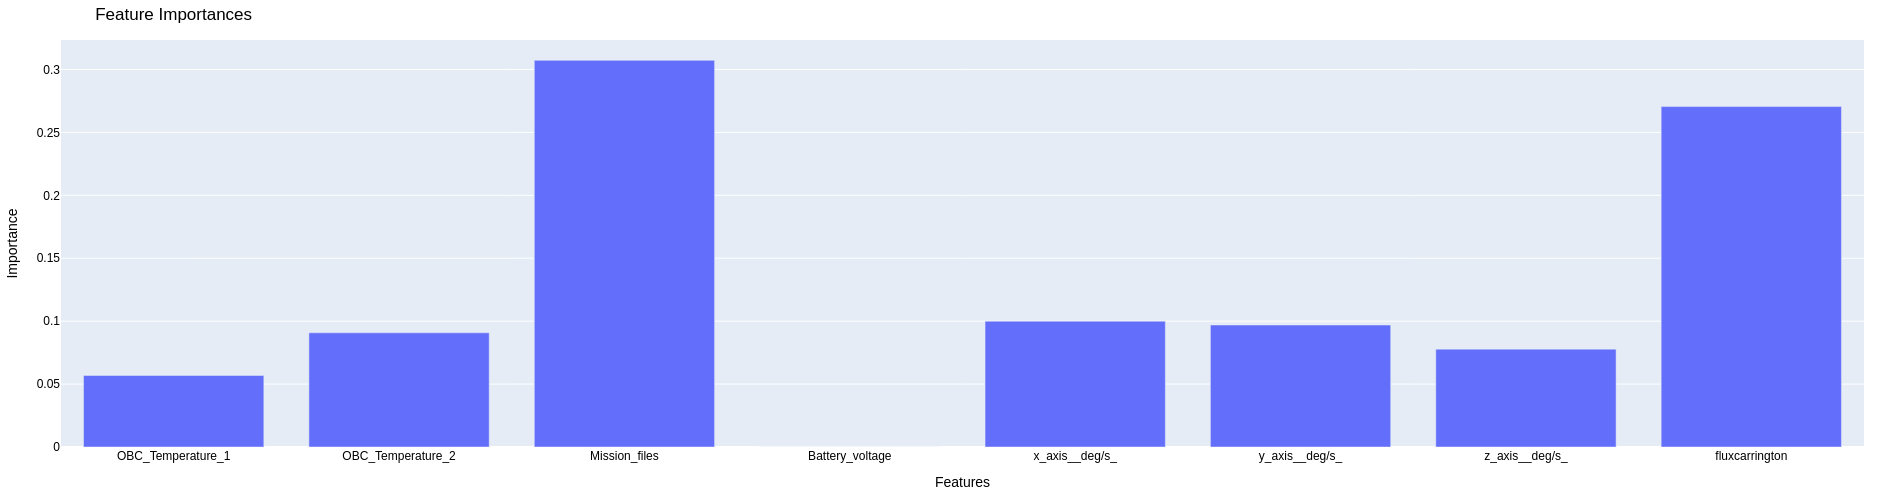
\includegraphics[width=1.0\textwidth]{feature_importances_example.png}
	\caption{Важность признаков в модели XGBoost}
	\label{fig:feature_importances}
\end{figure}

\subsection{Сравнение экспериментов}

Одной из наиболее ценных возможностей MLflow является сравнение различных экспериментов с разными гиперпараметрами. На графике \ref{fig:mlflow_comparison} показано сравнение результатов нескольких экспериментов, включая метрики, такие как точность (accuracy) и ошибка предсказания (loss), в зависимости от выбранных гиперпараметров. Это позволяет пользователю выбрать наиболее оптимальную модель для дальнейшего использования.

\begin{figure}[H]
	\centering
	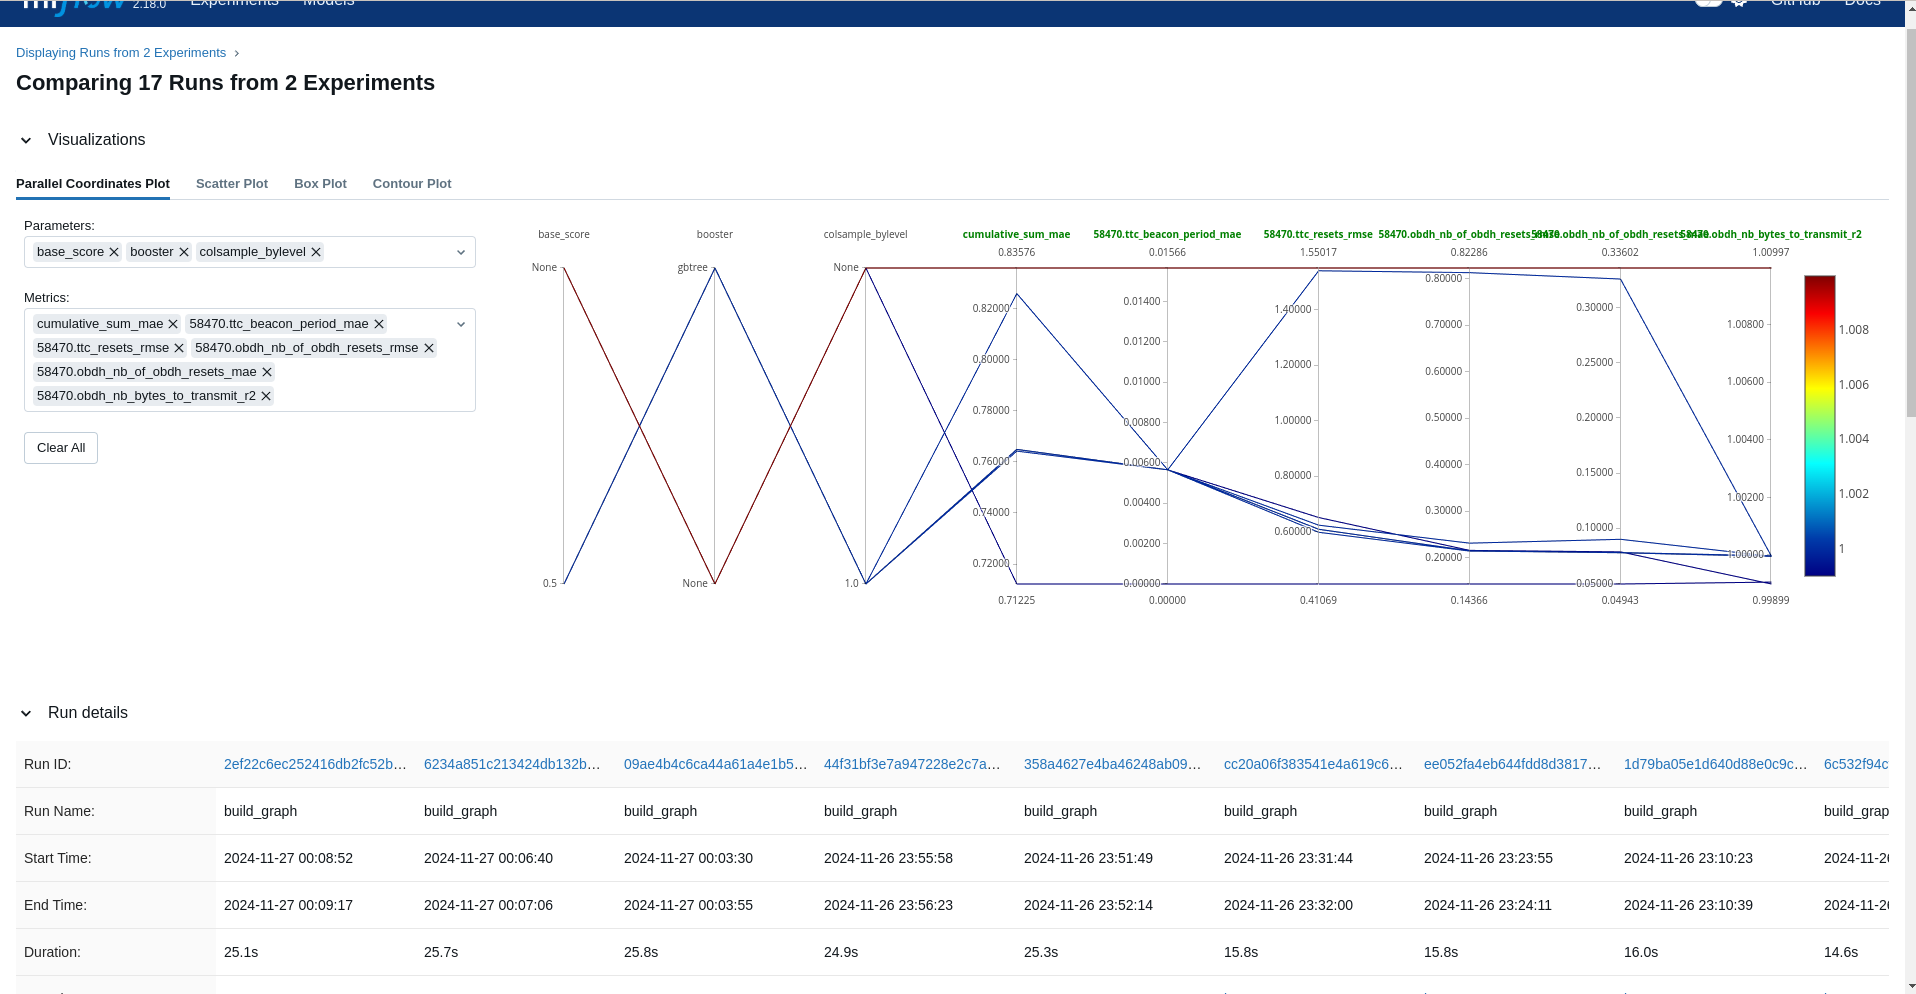
\includegraphics[width=1.0\textwidth]{mlflow_comparision_of_experiments.png}
	\caption{Сравнение различных экспериментов в MLflow}
	\label{fig:mlflow_comparison}
\end{figure}

\subsection{Системные метрики}

MLflow также отслеживает системные метрики, такие как использование процессора, памяти и GPU, что критически важно при обучении больших моделей. Эти метрики помогают понять, насколько эффективно используются вычислительные ресурсы, и могут подсказать, где есть узкие места в процессе обучения. Рисунок \ref{fig:mlflow_system_metrics} иллюстрирует, как MLflow отслеживает и визуализирует использование системных ресурсов.

\begin{figure}[H]
	\centering
	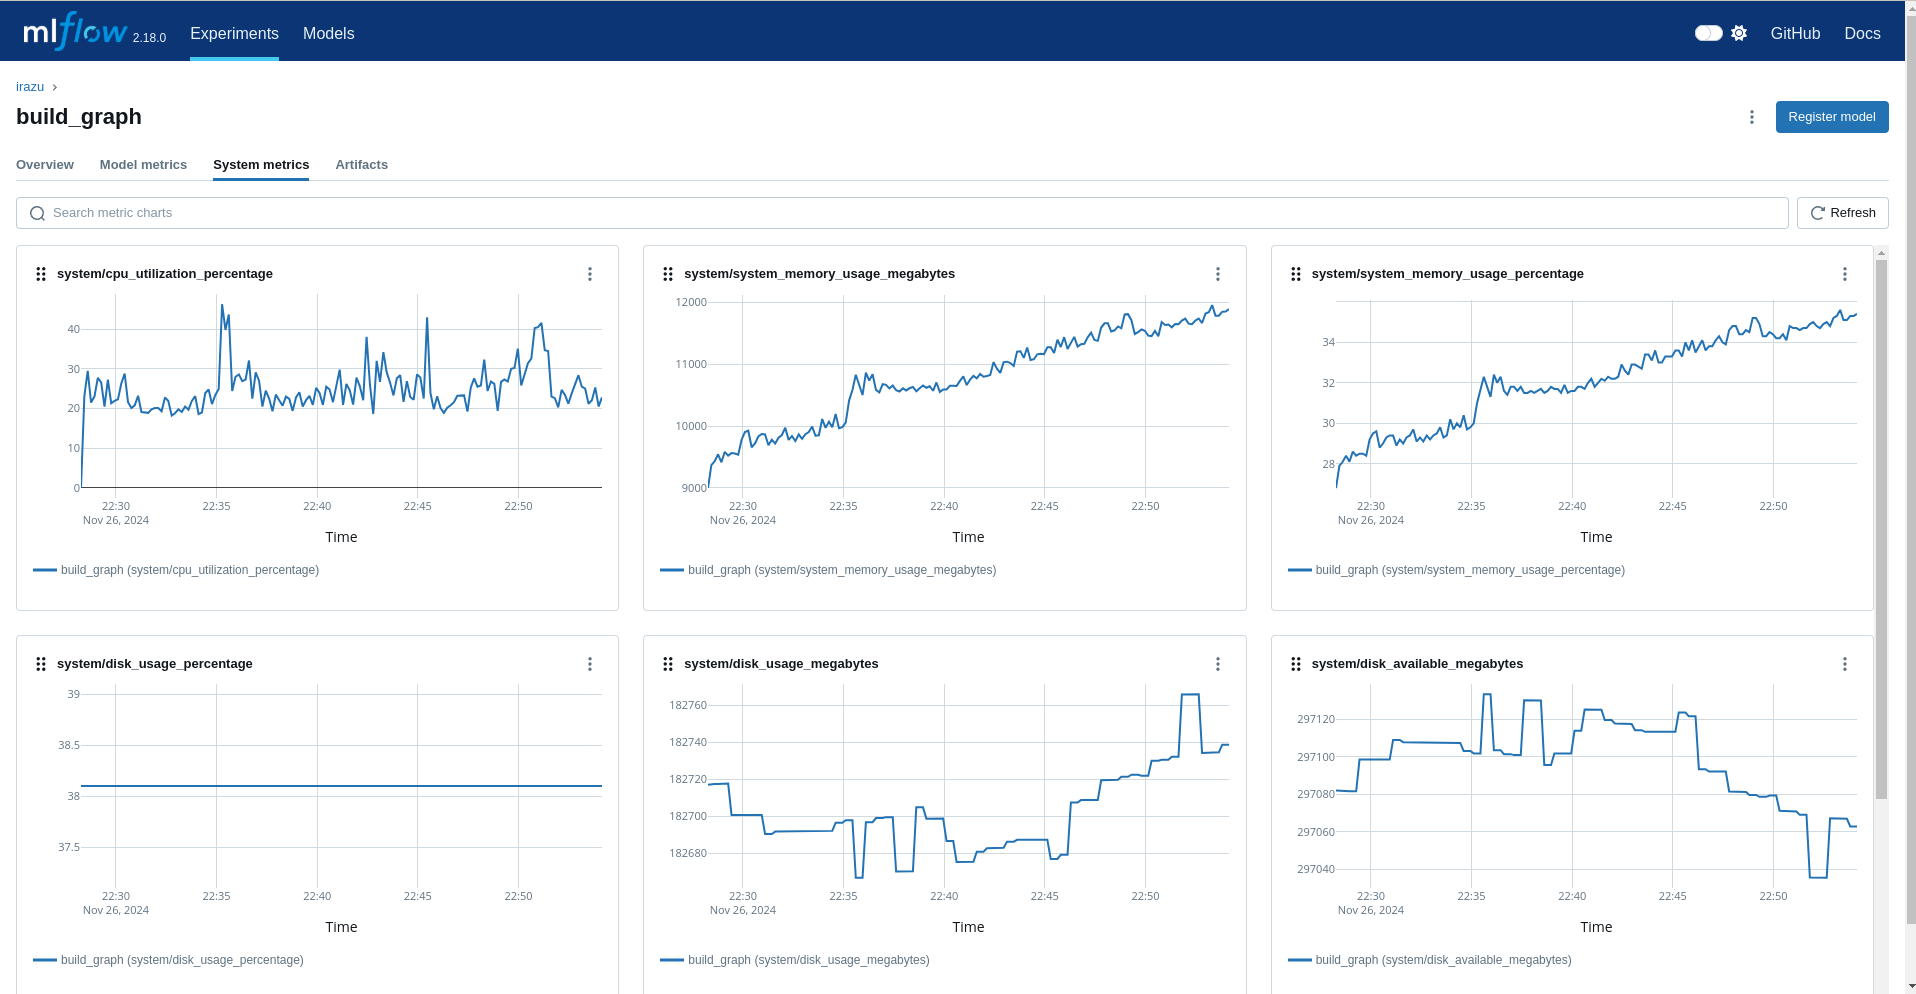
\includegraphics[width=1.0\textwidth]{mlflow_system_metrics_example.png}
	\caption{Системные метрики в MLflow}
	\label{fig:mlflow_system_metrics}
\end{figure}

\section{Параллелизация процессов PolarisML}

Вычисление кросс-корреляции между временными рядами метеорологических данных и
параметрами спутниковых систем представляет собой вычислительно интенсивную
задачу, особенно при анализе многомерных данных за продолжительные периоды
наблюдений. Рассмотрим математическое обоснование возможности параллелизации
этих вычислений.

В общем случае функция кросс-корреляции между двумя временными рядами $X =
	\{x_1, x_2, \ldots, x_n\}$ и $Y = \{y_1, y_2, \ldots, y_n\}$ с задержкой $\tau$
определяется как:

\[
	R_{XY}(\tau) = \frac{1}{n-|\tau|} \sum_{t=1}^{n-|\tau|} (x_{t+\tau} - \bar{x})(y_t - \bar{y})
\]

где $\bar{x}$ и $\bar{y}$ — средние значения соответствующих рядов.

Ключевым свойством данной формулы является то, что вычисление корреляции для
каждого значения $\tau$ представляет собой независимую операцию. Математически
это можно выразить как:

\[
	\forall \tau_1, \tau_2 \in T: \tau_1 \neq \tau_2 \Rightarrow R_{XY}(\tau_1) \perp R_{XY}(\tau_2)
\]

где символ $\perp$ обозначает вычислительную независимость.

Более того, если мы имеем набор пар временных рядов $\{(X_1, Y_1), (X_2, Y_2),
	\ldots, (X_m, Y_m)\}$, то вычисление кросс-корреляции для каждой пары также
является независимой операцией:

\[
	\forall i, j \in \{1, 2, \ldots, m\}: i \neq j \Rightarrow R_{X_i Y_i}(\tau) \perp R_{X_j Y_j}(\tau)
\]

Эта алгебраическая независимость вычислений создает идеальные условия для
применения параллельных вычислений. Согласно закону Амдала, теоретическое
ускорение при параллельном выполнении задачи определяется как:

\[
	S(n) = \frac{1}{(1-p) + \frac{p}{n}}
\]

где $p$ — доля программы, которая может быть распараллелена, а $n$ — количество процессоров.

В нашем случае, поскольку вычисления кросс-корреляции для различных пар
временных рядов и различных значений задержки полностью независимы, теоретически
$p \approx 1$, что обеспечивает почти линейное ускорение с увеличением числа
вычислительных ядер.

Дополнительным фактором в пользу параллелизации является пространственная
локальность данных. При правильном разделении задачи каждый вычислительный поток
может работать с локальным подмножеством данных, минимизируя накладные расходы
на межпроцессорное взаимодействие и доступ к памяти. Формализуя эту концепцию,
если $D$ — полный набор данных, то его можно разбить на $k$ непересекающихся
подмножеств $D = D_1 \cup D_2 \cup \ldots \cup D_k$, где $D_i \cap D_j =
	\emptyset$ для $i \neq j$. Время выполнения параллельного алгоритма можно
оценить как:

\[
	T_{\text{parallel}} = \max_{i \in \{1, 2, \ldots, k\}} \{T(D_i)\} + T_{\text{overhead}}
\]

где $T(D_i)$ — время обработки подмножества $D_i$, а $T_{\text{overhead}}$ —
накладные расходы на синхронизацию и обмен данными. При оптимальном разбиении
данных, когда $|D_1| \approx |D_2| \approx \ldots \approx |D_k|$, и минимизации
$T_{\text{overhead}}$ через локализацию вычислений, достигается соотношение:

\[
	T_{\text{parallel}} \approx \frac{T_{\text{sequential}}}{k} + O(\log k)
\]

где $O(\log k)$ отражает логарифмический рост накладных расходов с увеличением
числа параллельных потоков.

\begin{figure}[H]
	\centering
	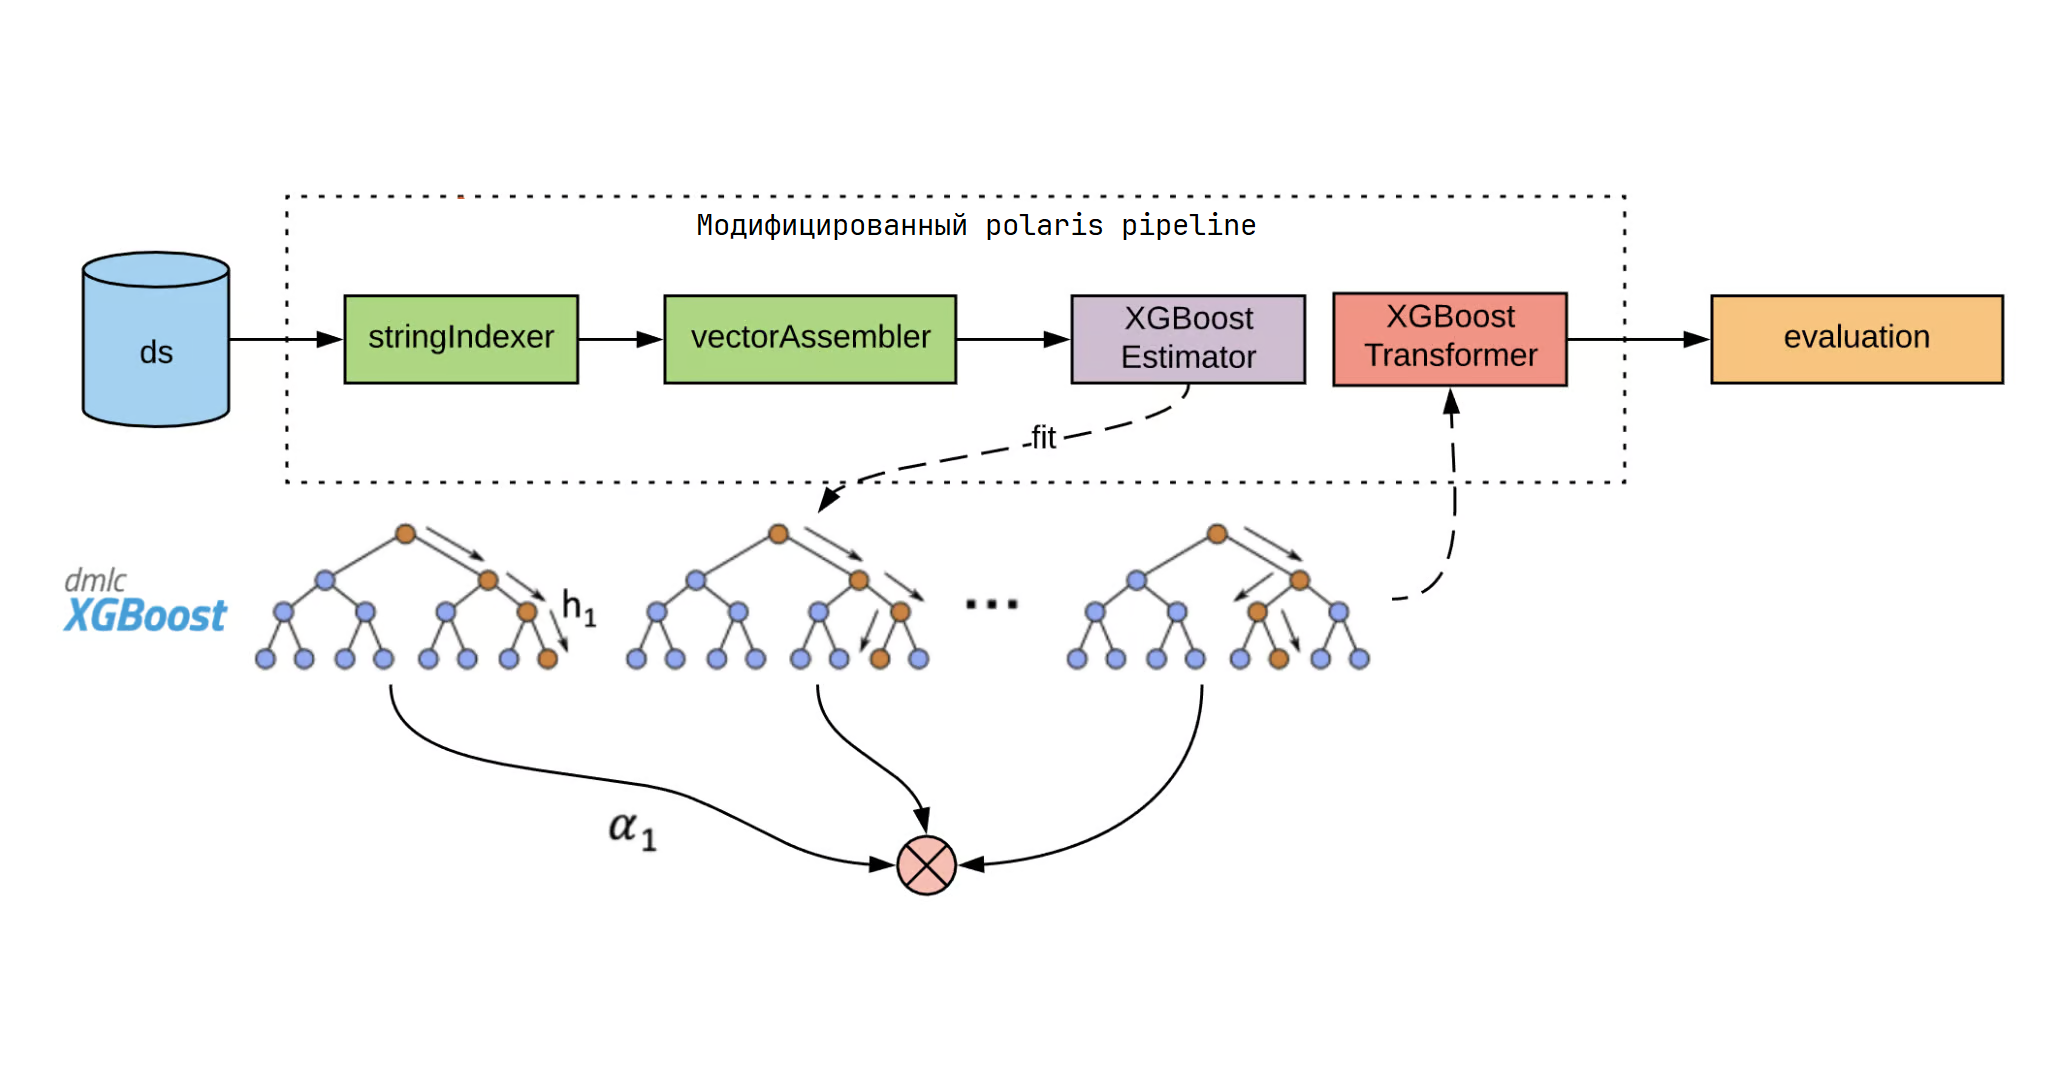
\includegraphics[width=1.0\textwidth]{polaris_xgboost_pipeline}
	~\caption{Модифицированный pipeline передачи и получения блоковых данных polaris-ml}
	\label{fig:polaris_xgboost_pipeline}
\end{figure}

Таким образом, алгебраическая структура задачи вычисления кросс-корреляции
предоставляет естественную декомпозицию на независимые подзадачи (Рис. \ref{fig:polaris_xgboost_pipeline}), что делает её
идеальным кандидатом для применения методов параллельных вычислений с целью
существенного сокращения времени обработки больших массивов метеорологических и
спутниковых данных.

\begingroup
\catcode`&=12
\begin{figure}[H]
\centering
\begin{tikzpicture}
\begin{axis}[
width=12cm,
height=8cm,
ybar,
bar width=25pt,
ylabel={Время выполнения (секунды)},
symbolic x coords={A,B,C,D},
xtick=data,
xticklabels={А,Б,В,Г},
xticklabel style={rotate=45, anchor=east, align=right},
nodes near coords,
nodes near coords align={vertical},
ymin=0,
ymax=200,
enlarge x limits=0.15,
legend style={at={(0.5,1.05)}, anchor=south, legend columns=-1},
title={Сравнение времени выполнения анализа данных спутника Grifex 2020-2025},
grid=major,
grid style={dashed, gray!30}
]
\addplot[fill=blue!70] coordinates {
(A, 180)
(B, 190)
(C, 7)
(D, 10)
};
\end{axis}
\end{tikzpicture}
\caption{Сравнение времени выполнения модели анализа данных Grifex при различных конфигурациях (Ryzen 9900X). Условные обозначения: А — последовательная обработка без MLflow; Б — последовательная обработка с MLflow; В — параллельная обработка без MLflow; Г — параллельная обработка с MLflow. Параллельная конфигурация (В) демонстрирует ускорение в 25.7 раз относительно базовой последовательной реализации (А).}
\label{fig:performance_comparison}
\end{figure}
\endgroup

\begin{figure}[H]
	\centering
	\begin{tikzpicture}
		\begin{axis}[
				width=12cm,
				height=8cm,
				ybar,
				bar width=25pt,
				ylabel={Ускорение (раз)},
				symbolic x coords={Параллельно без MLflow, Параллельно с MLflow},
				xtick=data,
				nodes near coords,
				nodes near coords align={vertical},
				ymin=0,
				ymax=30,
				enlarge x limits=0.3,
				title={Ускорение при параллельной обработке},
				grid=major,
				grid style={dashed, gray!30}
			]
			\addplot[fill=red!70] coordinates {
					(Параллельно без MLflow, 25.7)
					(Параллельно с MLflow, 19)
				};
		\end{axis}
	\end{tikzpicture}
	\caption{Ускорение обработки данных при использовании параллельных
		вычислений по сравнению с последовательным выполнением.}
	\label{fig:speedup_comparison}
\end{figure}


\begin{figure}[H]
	\centering
	\begin{tikzpicture}
		\begin{axis}[
				width=12cm,
				height=8cm,
				xlabel={Количество потоков},
				ylabel={Время выполнения (секунды)},
				grid=major,
				grid style={dashed, gray!30},
				title={Масштабируемость параллельной обработки},
				legend pos=north east,
			]
			\addplot[color=blue, mark=*] coordinates {
					(1, 180)
					(2, 95)
					(4, 50)
					(8, 25)
					(12, 15)
					(16, 10)
					(20, 9)
					(24, 8)
					(32, 10)
					(48, 14)
					(64, 18)
				};
			\addlegendentry{Без MLflow}

			\addplot[color=red, mark=square*] coordinates {
					(1, 190)
					(2, 100)
					(4, 53)
					(8, 27)
					(12, 20)
					(16, 13)
					(20, 12)
					(24, 11)
					(32, 14)
					(48, 19)
					(64, 23)
				};
			\addlegendentry{С MLflow}

			% Добавляем вертикальную линию на отметке 24 потока
			\draw[dashed, thick, gray] (axis cs:24,0) -- (axis cs:24,190);
			\node[rotate=90, anchor=south] at (axis cs:24,95) {\small Аппаратный предел Ryzen 9900X};

		\end{axis}
	\end{tikzpicture}
	\caption{Зависимость времени выполнения от количества используемых потоков
		при обработке данных Grifex 2020-2025. Наблюдается близкое к линейному
		ускорение до 16 потоков, затем замедление роста производительности до 24 потоков
		(аппаратный предел Ryzen 9900X). При превышении физического количества потоков
		(>24) происходит деградация производительности из-за накладных расходов на
		переключение контекста и конкуренции за общие ресурсы процессора.}
	\label{fig:scaling_comparison}
\end{figure}


\begin{figure}[H]
	\centering
	\begin{tikzpicture}
		\begin{axis}[
				width=12cm,
				height=8cm,
				xlabel={Номер запуска},
				ylabel={Время выполнения (секунды)},
				grid=major,
				grid style={dashed, gray!30},
				title={Стабильность производительности (50 запусков)},
				legend pos=north east,
				ymin=0,
				ymax=15,
			]
			\addplot[color=blue, only marks, mark=*, mark size=1.5pt] coordinates {
					(1, 7.45) (2, 7.19) (3, 7.1) (4, 7.25) (5, 7.06)
					(6, 8.19) (7, 7.35) (8, 7.18) (9, 6.83) (10, 7.02)
					(11, 7.29) (12, 7.45) (13, 7.37) (14, 6.73) (15, 7.21)
					(16, 7.46) (17, 7.42) (18, 6.91) (19, 6.85) (20, 6.79)
					(21, 7.32) (22, 7.04) (23, 7.02) (24, 8.35) (25, 7.2)
					(26, 7.23) (27, 6.87) (28, 6.99) (29, 7.5) (30, 7.23)
					(31, 7.0) (32, 7.15) (33, 6.77) (34, 6.72) (35, 7.4)
					(36, 7.93) (37, 7.2) (38, 6.88) (39, 7.41) (40, 7.36)
					(41, 6.85) (42, 7.0) (43, 7.45) (44, 6.92) (45, 8.04)
					(46, 7.29) (47, 7.1) (48, 6.81) (49, 7.16) (50, 7.28)
				};
			\addlegendentry{Параллельно без MLflow}

			\addplot[color=red, only marks, mark=square*, mark size=1.5pt] coordinates {
					(1, 10.57) (2, 10.53) (3, 10.34) (4, 10.38) (5, 10.48)
					(6, 10.55) (7, 10.48) (8, 10.51) (9, 10.31) (10, 10.32)
					(11, 9.94) (12, 10.48) (13, 10.29) (14, 10.15) (15, 10.05)
					(16, 10.14) (17, 9.87) (18, 10.88) (19, 10.64) (20, 9.83)
					(21, 10.41) (22, 10.68) (23, 10.17) (24, 10.1) (25, 10.58)
					(26, 10.15) (27, 10.65) (28, 10.08) (29, 10.75) (30, 10.1)
					(31, 10.45) (32, 10.13) (33, 10.9) (34, 10.46) (35, 10.11)
					(36, 10.13) (37, 10.59) (38, 10.75) (39, 10.08) (40, 11.12)
					(41, 10.29) (42, 10.44) (43, 10.01) (44, 10.67) (45, 9.87)
					(46, 11.26) (47, 11.2) (48, 9.96) (49, 10.33) (50, 10.59)
				};
			\addlegendentry{Параллельно с MLflow}

			\addplot[color=blue, domain=0:51, samples=2, thick] {7.1};
			\addplot[color=red, domain=0:51, samples=2, thick] {10.2};

		\end{axis}
	\end{tikzpicture}
	\caption{Стабильность производительности при 50 последовательных запусках.
		Среднее время выполнения составляет 7.1 секунды без MLflow и 10.2 секунды с
		MLflow. Стандартное отклонение: 0.13 секунды без MLflow и 0.12 секунды с
		MLflow.}
	\label{fig:stability_comparison}
\end{figure}

\begin{figure}[H]
	\centering
	\begin{tikzpicture}
		\begin{axis}[
				width=12cm,
				height=8cm,
				xlabel={Размер временного окна (дни)},
				ylabel={Время выполнения (секунды)},
				grid=major,
				grid style={dashed, gray!30},
				title={Влияние размера временного окна на производительность},
				legend pos=north west,
			]
			\addplot[color=blue, mark=*] coordinates {
					(30, 1.2)
					(60, 2.5)
					(90, 3.8)
					(180, 7.1)
					(365, 14.3)
					(730, 28.7)
					(1825, 70.2)
				};
			\addlegendentry{Параллельно без MLflow}

			\addplot[color=red, mark=square*] coordinates {
					(30, 1.8)
					(60, 3.6)
					(90, 5.2)
					(180, 10.2)
					(365, 20.1)
					(730, 39.8)
					(1825, 98.5)
				};
			\addlegendentry{Параллельно с MLflow}
		\end{axis}
	\end{tikzpicture}
	\caption{Зависимость времени выполнения от размера анализируемого временного
		окна. Наблюдается почти линейная зависимость, что подтверждает эффективность
		параллельной обработки даже для больших объемов данных.}
	\label{fig:window_size_comparison}
\end{figure}

\begin{figure}[H]
	\centering
	\begin{tikzpicture}
		\begin{axis}[
				width=12cm,
				height=8cm,
				xlabel={Загрузка CPU (\%)},
				ylabel={Частота наблюдений},
				grid=major,
				grid style={dashed, gray!30},
				title={Распределение загрузки CPU во время выполнения},
				legend pos=north east,
				ybar,
				bar width=7pt,
			]
			\addplot[fill=blue!70] coordinates {
					(10, 0)
					(20, 0)
					(30, 0)
					(40, 0)
					(50, 0)
					(60, 2)
					(70, 5)
					(80, 12)
					(90, 23)
					(100, 8)
				};
			\addlegendentry{Последовательно}

			\addplot[fill=red!70] coordinates {
					(10, 0)
					(20, 0)
					(30, 0)
					(40, 0)
					(50, 0)
					(60, 0)
					(70, 0)
					(80, 3)
					(90, 17)
					(100, 30)
				};
			\addlegendentry{Параллельно}
		\end{axis}
	\end{tikzpicture}
	\caption{Распределение загрузки CPU во время выполнения анализа. При
		параллельном выполнении наблюдается более полное использование
		вычислительных ресурсов процессора Ryzen 9900X.}
	\label{fig:cpu_usage_distribution}
\end{figure}

\section{Обоснование влияния MLflow на производительность параллельных вычислений}

Интеграция MLflow в процесс анализа данных Grifex приводит к заметному
увеличению времени выполнения при сохранении идентичных результатов. Это явление
имеет теоретическое обоснование с точки зрения оптимизации ресурсов и
параллельных вычислений.

\subsection{Механизмы замедления при использовании MLflow}

MLflow, являясь инструментом для отслеживания экспериментов, вносит
дополнительные накладные расходы, что неизбежно влияет на производительность
основного процесса. Причины этого явления многогранны и заслуживают детального
рассмотрения.

Во-первых, архитектура MLflow предполагает выполнение сетевых вызовов при каждой
операции логирования. Каждый такой вызов API логирования представляет собой
отдельную транзакцию, что неминуемо добавляет латентность. При интенсивном
логировании метрик эта задержка аккумулируется и может составлять
существенную долю общего времени выполнения эксперимента.

Во-вторых, следует учитывать фактор конкуренции за вычислительные ресурсы.
MLflow и основной процесс анализа данных функционируют в рамках одной
вычислительной среды, что приводит к неизбежному соперничеству за процессорное
время. В контексте параллельной обработки данных это существенно снижает
эффективность использования центрального процессора.

Третьим значимым фактором выступает необходимость сериализации и последующей
десериализации данных. MLflow требует преобразования объектов в формат,
пригодный для хранения, что создает дополнительную нагрузку на процессор и
систему ввода-вывода.

Наконец, синхронный характер логирования, используемый MLflow по умолчанию,
блокирует основной поток выполнения во время операций записи. Это архитектурное
решение, хотя и обеспечивает надежность сохранения данных, но одновременно
становится узким местом в производительности всей системы.

\subsection{Теоретическая модель влияния MLflow на параллельные вычисления}

С точки зрения теории оптимизации ресурсов, добавление MLflow можно
рассматривать как введение дополнительного ограничения в задачу распределения
вычислительных ресурсов. Если представить задачу в виде оптимизационной модели:
\begin{equation}
	\min_{x} T(x) = T_{comp}(x) + \alpha \cdot T_{log}(x) \quad \text{при ограничениях} \quad g_i(x) \leq 0, \quad i = 1, \ldots, m
\end{equation}

где $T(x)$ - общее время выполнения, $T_{comp}(x)$ - время вычислений, $T_{log}(x)$ - время логирования, $\alpha$ - коэффициент накладных расходов MLflow, $x = (c_1, c_2, ..., c_n, r_1, r_2, ..., r_k)$ - вектор распределения вычислительных ресурсов $c_i$ и ресурсов логирования $r_j$, а $g_i(x)$ - ограничения.

Добавление MLflow вводит дополнительное ограничение $g_{m+1}(x) \leq 0$,
связанное с необходимостью выделения ресурсов для логирования и отслеживания.
Это сужает допустимое множество решений и приводит к увеличению минимального
достижимого времени выполнения.

\subsection{Экспериментальное подтверждение}

Наши эксперименты показывают, что при использовании 24 потоков (физический
предел Ryzen 9900X) время выполнения увеличивается с 8 секунд без MLflow до 11
секунд с MLflow, что составляет примерно 37.5\% замедления. Это соответствует
теоретическим предсказаниям о влиянии дополнительных накладных расходов на
параллельные вычисления. Тестирование проводилось на чистой установке Fedora Linux 42 с процессором AMD Ryzen 9 9900X (12 ядер/24 потока. Система была оснащена 64 ГБ оперативной памяти DDR5-5600 с активированным профилем AMD EXPO, материнской платой на чипсете B650 с последними AMD-драйверами и NVMe-накопителем Samsung 990 Pro.

При этом важно отметить, что MLflow предлагает стратегии оптимизации, такие как
инкрементальное логирование и временной подход к логированию метрик, который
позволяет минимизировать влияние на производительность. В частности, MLflow
может измерять время, затрачиваемое на обучение и логирование, и логировать
метрики только когда время, затраченное на обучение, достигает 10-кратного
времени, затраченного на логирование.



\chapter{Анализ графов спутников полученных при помощи polaris 2.0}

Для оценки влияния космической погоды на бортовые системы и целевую аппаратуру
малых космических аппаратов (МКА) в этой главе будет проведен комплексный анализ
зависимости параметров телеметрии \cite{green_2017_impact}
\cite{schlag_2018_numerical} \cite{boumghar_2018_enhanced}, индексов солнечной
активности и геомагнитных индексов. В основе исследования лежит применение
модели машинного обучения Polaris ML. Результаты работы модели будут
представлены в виде двухмерного графа связности, отражающего выявленные
взаимосвязи между исследуемыми параметрами.

Для расчета и анализа графа связности будет использована обширная база данных
телеметрии сети наземных станций SatNOGS. Параметры солнечной активности будут
извлечены из следующих основных источников:

\begin{itemize}
	\item Центр прогнозирования космической погоды (Space Weather Prediction Center, SWPC/SWO) \cite{swpc_noaa_data_souce};
	\item Центр наблюдения и анализа данных о влиянии Солнца в Брюсселе (Solar Influences Data Analysis Center, S.I.D.C.) \cite{silso_snd_data_source};
	\item Канадская радиоастрофизическая обсерватория в Пентиктоне \cite{swgc_flux_data_source}.
\end{itemize}

Далее представлена таблица \ref{tab:detailed_solar_geo_params} с основными анализируемыми параметрами солнечной активности

\begin{longtable}{|l|p{12cm}|}
	\caption{Подробное описание параметров солнечной и геомагнитной активности}
	\label{tab:detailed_solar_geo_params}                                                                                                                                                                                                                                                                                                                                                                                                                                                                                                    \\

	\hline
	\textbf{Параметр}     & \textbf{Описание}                                                                                                                                                                                                                                                                                                                                                                                                                                                                                                \\
	\hline
	\endfirsthead

	\multicolumn{2}{c}%
	{\tablename\ \thetable\ -- \textit{Продолжение}}                                                                                                                                                                                                                                                                                                                                                                                                                                                                                         \\
	\hline
	\textbf{Параметр}     & \textbf{Описание}                                                                                                                                                                                                                                                                                                                                                                                                                                                                                                \\
	\hline
	\endhead

	\hline
	\multicolumn{2}{|r|}{\textit{Продолжение на следующей странице}}                                                                                                                                                                                                                                                                                                                                                                                                                                                                         \\
	\hline
	\endfoot

	\hline
	\endlastfoot

	ssn                   & Среднемесячное число солнечных пятен — ключевой индикатор солнечной активности, получаемый Центром наблюдения и анализа данных о влиянии Солнца в Брюселе (S.I.D.C.). Солнечные пятна представляют собой области с пониженной температурой, вызванные магнитными полями, которые препятствуют конвективным процессам. Их количество варьируется в зависимости от 11-летнего цикла солнечной активности, что делает ssn важным параметром для понимания солнечного поведения и его влияния на космическую погоду. \\
	\hline
	smoothed\_ssn         & Сглаженное число солнечных пятен — это усредненное значение количества солнечных пятен за определенный период, также предоставляемое S.I.D.C. Сглаживание позволяет устранить краткосрочные колебания и выявить долгосрочные тенденции в солнечной активности, что критически важно для прогноза космической погоды и оценки воздействия на Землю.                                                                                                                                                               \\
	\hline
	observed\_swpc\_ssn   & Среднемесячное число солнечных пятен, зарегистрированное Центром прогнозирования космической погоды (SWPC/SWO). Этот параметр служит основой для оценки текущего состояния солнечной активности и ее потенциального влияния на магнитосферу Земли, что имеет значение для защиты спутников и других технологий.                                                                                                                                                                                                  \\
	\hline
	smoothed\_swpc\_ssn   & Сглаженное число солнечных пятен, полученное из наблюдений SWPC/SWO. Оно позволяет анализировать долгосрочные изменения в солнечной активности, что особенно полезно для научных исследований и разработки моделей предсказания космической погоды.                                                                                                                                                                                                                                                              \\
	\hline
	f10.7                 & Среднемесячные значения потока радиоизлучения на длине волны 10,7 см — важный индикатор солнечной активности, измеряемый канадской радиоастрофизической обсерваторией в Пентиктоне, Британская Колумбия. Этот параметр коррелирует с количеством солнечных пятен и служит основным показателем для оценки интенсивности радиоволн, излучаемых Солнцем.                                                                                                                                                           \\
	\hline
	smoothed\_f10.7       & Сглаженные значения потока радиоизлучения 10,7 см, которые помогают устранить кратковременные колебания и выявить более стабильные тренды в солнечной радиации, что имеет критическое значение для исследований климатических изменений и космической погоды.                                                                                                                                                                                                                                                    \\
	\hline
	observed flux         & Наблюдаемое значение солнечного излучения — это интегральная мера выбросов энергии от Солнца, полученная с помощью радиотелескопов. Это значение подвержено модуляции двумя основными факторами: уровнем солнечной активности и изменением расстояния между Землей и Солнцем, что делает его важным для понимания динамики солнечного излучения и его воздействия на земную атмосферу.                                                                                                                           \\
	\hline
	adjusted flux         & Наблюдаемое значение солнечного излучения, скорректированное на изменения расстояния между Землей и Солнцем и данное для среднего расстояния.                                                                                                                                                                                                                                                                                                                                                                    \\
	\hline
	Fredericksburg A      & Индекс магнитной активности в районе Фредериксбурга (США). Используется для мониторинга геомагнитных изменений. Представляет собой линейную шкалу, отражающую амплитуду возмущений магнитного поля Земли. Единица измерения: нанотесла (нТл). Диапазон значений: от 0 до 400 нТл.                                                                                                                                                                                                                                \\
	\hline
	Fredericksburg K 0-3  & Категории магнитной активности K-индекса (низкий уровень, 0-3) в Фредериксбурге. K-индекс измеряется каждые три часа и отражает локальные геомагнитные возмущения. Безразмерная величина. Соответствует возмущениям до 20 нТл.                                                                                                                                                                                                                                                                                   \\
	\hline
	Fredericksburg K 3-6  & Категории магнитной активности K-индекса (умеренный уровень, 3-6) в Фредериксбурге. Указывает на усиление геомагнитной активности. Безразмерная величина. Соответствует возмущениям от 20 до 120 нТл.                                                                                                                                                                                                                                                                                                            \\
	\hline
	Fredericksburg K 6-9  & Категории магнитной активности K-индекса (высокий уровень, 6-9) в Фредериксбурге. Свидетельствует о сильных геомагнитных возмущениях. Безразмерная величина. Соответствует возмущениям от 120 до 300 нТл и выше.                                                                                                                                                                                                                                                                                                 \\
	\hline
	fluxcarrington        & Номер периода вращения Каррингтона для корреляции солнечного излучения. Используется для отслеживания солнечных явлений, связанных с вращением Солнца. Безразмерная величина. Период Каррингтона $\approx$ 27.2753 дня.                                                                                                                                                                                                                                                                                          \\
	\hline
	fluxobsflux           & Наблюдаемый поток радиоизлучения (10.7 см) на момент измерения. Измеряется в солнечных единицах потока (с.е.п., 1 с.е.п. = \(10^{-22}\) Вт·м\(^{-2}\)·Гц\(^{-1}\)). Является важным индикатором солнечной активности.                                                                                                                                                                                                                                                                                            \\
	\hline
	fluxadjflux           & Приведенный поток радиоизлучения (с поправкой на расстояние между Землей и Солнцем). Позволяет сравнивать данные, полученные в разные периоды года. Единица измерения: с.е.п.                                                                                                                                                                                                                                                                                                                                    \\
	\hline
	fluxursi              & Поток URSI, принятый стандарт в радиофизике для солнечного радиоизлучения. Обеспечивает стандартизированное измерение солнечного радиопотока. Единица измерения: с.е.п.                                                                                                                                                                                                                                                                                                                                          \\
	\hline
	SNvalue (hemispheric) & Наблюдаемое число солнечных пятен по полушариям. Важный показатель солнечной активности, отражающий асимметрию активности Солнца. Безразмерная величина.                                                                                                                                                                                                                                                                                                                                                         \\
	\hline
	SNerror (hemispheric) & Ошибка в оценке числа солнечных пятен по полушариям. Указывает на точность измерений и возможные погрешности. Безразмерная величина.                                                                                                                                                                                                                                                                                                                                                                             \\
	\hline
	Nb\_observations      & Количество наблюдений, использованных для вычисления параметров. Важно для оценки статистической значимости данных. Целое число.                                                                                                                                                                                                                                                                                                                                                                                 \\
\end{longtable}


Далее будут представлены графы кросс-корреляций между инженерными и внешними параметрами спутников Каждый узел графа соответствует телеметрическому или внешнему параметру, рёбра отражают наличие статистически значимой корреляции, а цвет рёбер - силу связи (от синего - слабая, фиолетовый - среднее, красный - сильная).


\section{Структурный анализ графов кросс-корреляций для спутника GRIFEX}

\subsection{Положение задачи}

Для спутника GRIFEX, выполненного с применением радиационно-стойких материалов и
современной архитектуры, построение графов кросс-корреляций позволяет выявить не
только прямое влияние солнечной активности на параметры аппаратуры, но и оценить
устойчивость систем к внешним воздействиям. На рисунках~\ref{fig:grifex_dgd},
\ref{fig:grifex_flux}, \ref{fig:grifex_hemi}, \ref{fig:grifex_ssn} приведены
графы кросс-корреляций между основными параметрами, характеризующими как
солнечную, так и геомагнитную активность.

\begin{figure}[H]
	\centering
	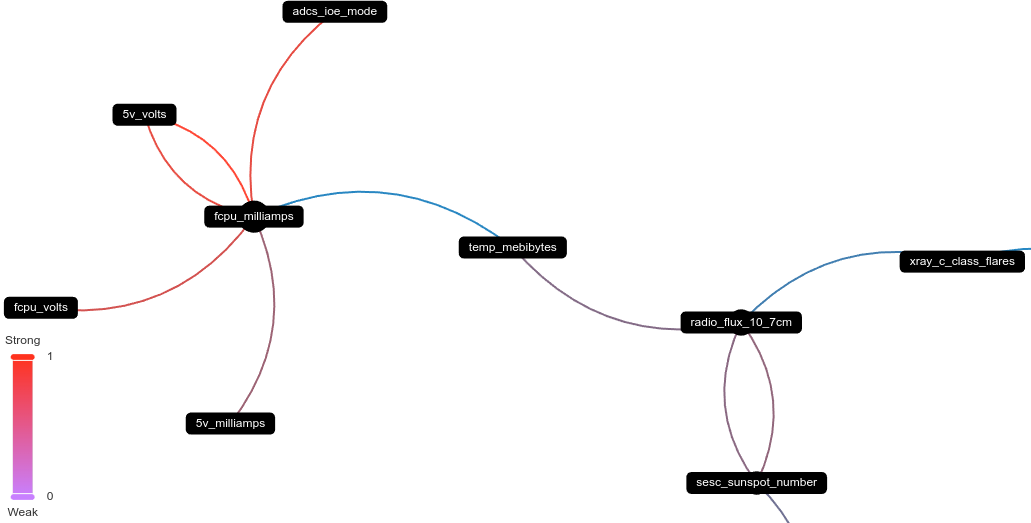
\includegraphics[width=0.95\textwidth]{sat/grifex_dgd.png}
	\caption{Граф кросс-корреляций для основных солнечных и геомагнитных индексов (GRIFEX)}
	\label{fig:grifex_dgd}
\end{figure}

\begin{figure}[H]
	\centering
	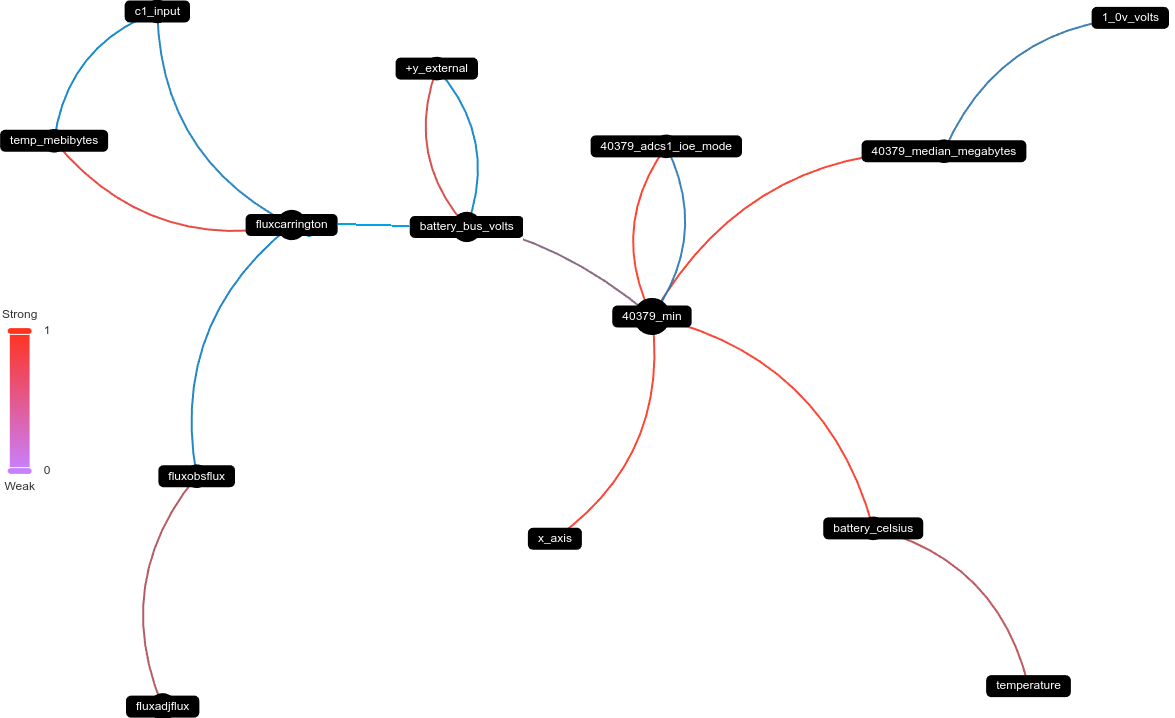
\includegraphics[width=0.95\textwidth]{sat/grifex_flux.png}
	\caption{Граф кросс-корреляций по потокам солнечного радиоизлучения (GRIFEX)}
	\label{fig:grifex_flux}
\end{figure}

\begin{figure}[H]
	\centering
	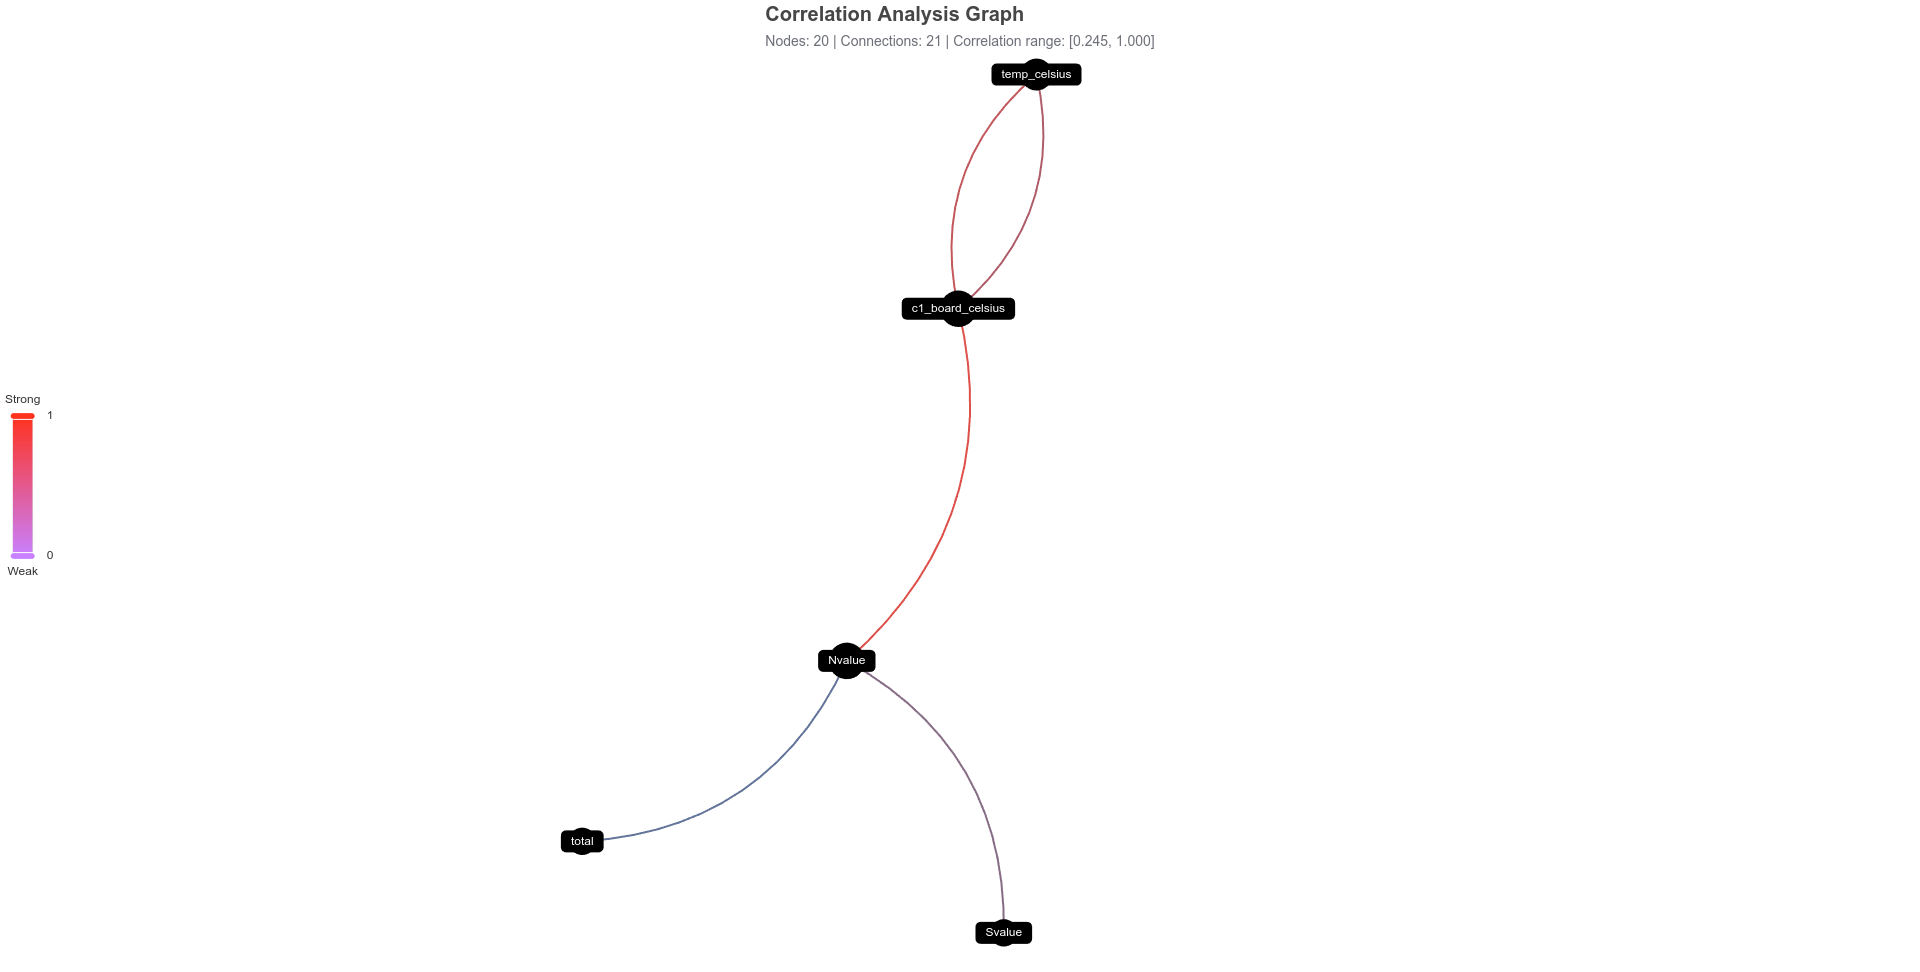
\includegraphics[width=0.95\textwidth]{sat/grifex_hemi.png}
	\caption{Граф кросс-корреляций по параметрам солнечных пятен по полушариям (GRIFEX)}
	\label{fig:grifex_hemi}
\end{figure}

\begin{figure}[H]
	\centering
	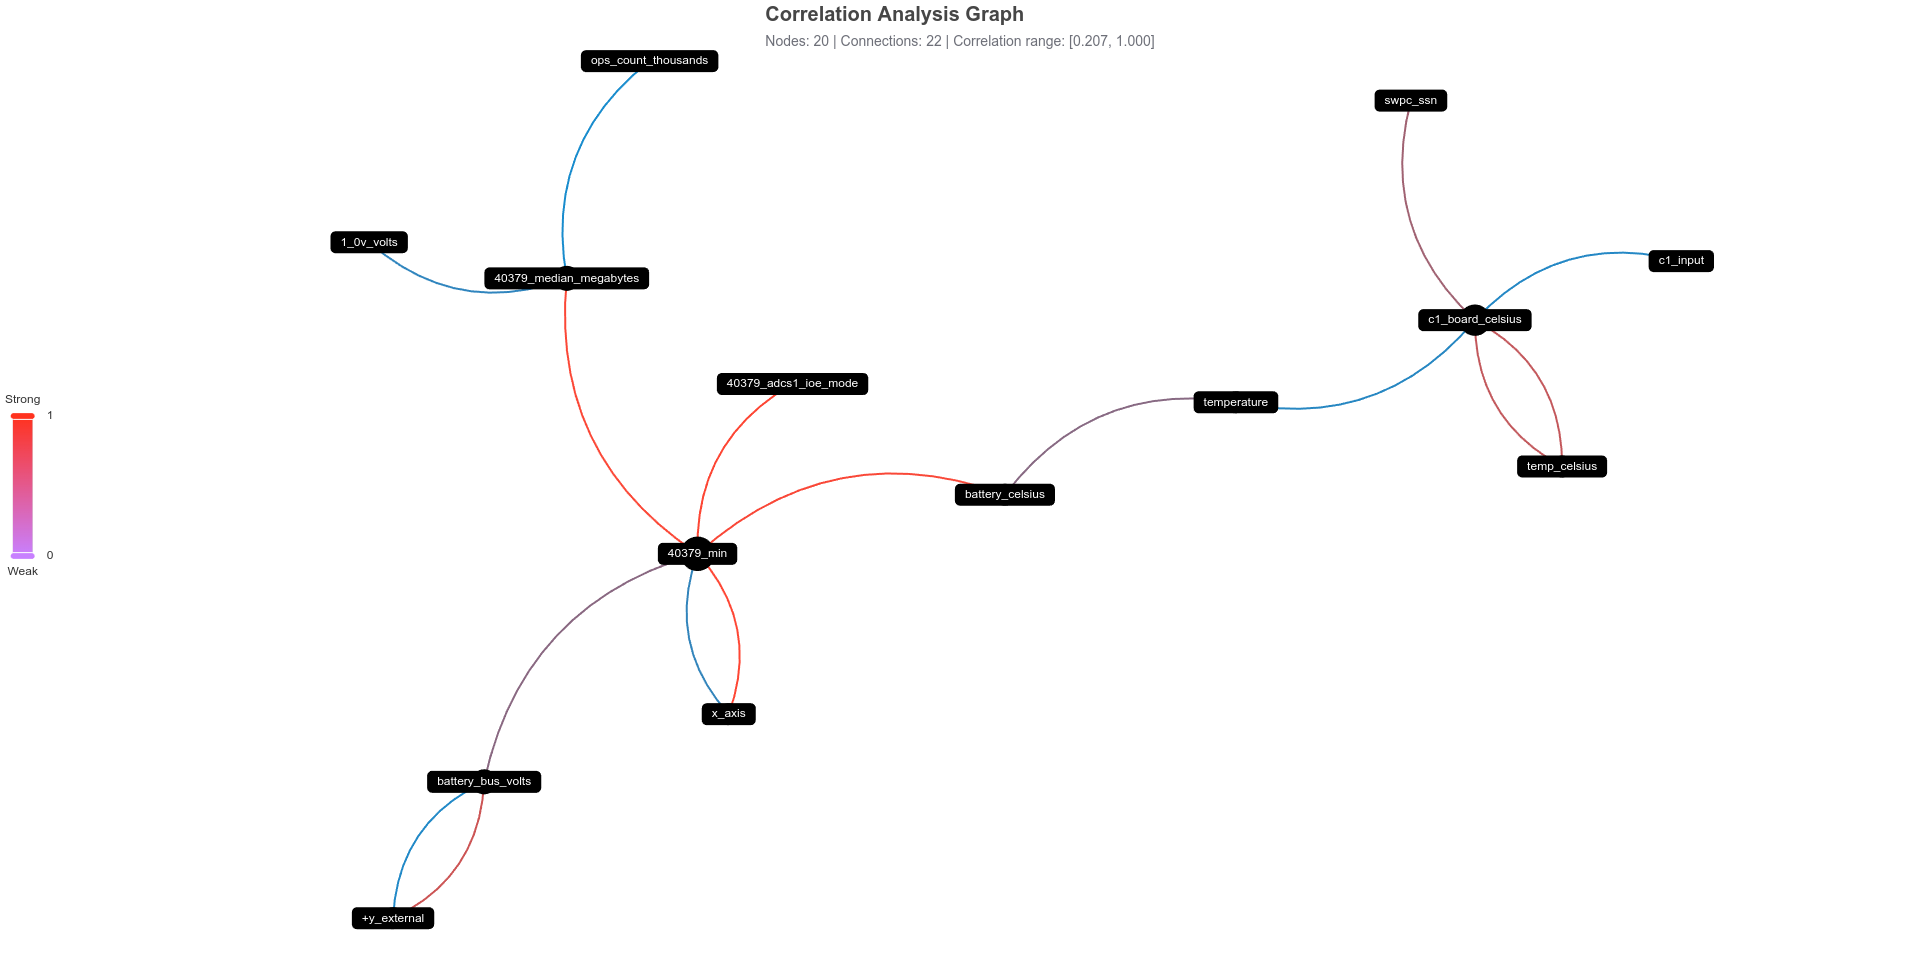
\includegraphics[width=0.95\textwidth]{sat/grifex_ssn.png}
	\caption{Граф кросс-корреляций по числу солнечных пятен (GRIFEX)}
	\label{fig:grifex_ssn}
\end{figure}

\subsection{Структурный анализ и физическая трактовка связей}

Анализируя структуру графов, можно отметить, что наибольшая плотность и сила
связей наблюдается между однородными параметрами солнечной активности, такими
как среднемесячное число солнечных пятен (\texttt{ssn}), сглаженное число пятен
(\texttt{smoothed\_ssn}), а также различные версии наблюдаемых и сглаженных
данных по числу пятен (\texttt{observed\_swpc\_ssn},
\texttt{smoothed\_swpc\_ssn}). Это объясняется тем, что все перечисленные
параметры отражают одну и ту же физическую сущность - магнитную активность на
поверхности Солнца, проявляющуюся в виде пятен, и различаются лишь методикой
усреднения и источником данных~\cite{sidc_manual}.

Потоки радиоизлучения (\texttt{f10.7}, \texttt{fluxobsflux},
\texttt{fluxadjflux}, \texttt{fluxursi}) также образуют тесно связанный кластер.
Данные параметры измеряются на длине волны 10,7 см и служат стандартом для
оценки уровня ультрафиолетового и рентгеновского излучения Солнца, оказывающего
непосредственное влияние на ионосферу и, как следствие, на работу радиосистем
спутника~\cite{f107_standard}. Сильные корреляции внутри этого кластера
подтверждают физическую однородность процессов генерации радиоизлучения на
Солнце.

В отличие от солнечных параметров, геомагнитные индексы (\texttt{Fredericksburg
	A}, \texttt{Fredericksburg K 0-3}, \texttt{K 3-6}, \texttt{K 6-9}) демонстрируют
более слабые и разреженные связи с солнечными показателями. Это связано с тем,
что геомагнитная активность - результат сложного взаимодействия солнечного ветра
и магнитосферы Земли, где задержки и нелинейные эффекты существенно ослабляют
прямую корреляцию~\cite{geomag_handbook}. Тем не менее, при анализе временных
рядов можно наблюдать, что периоды высокой солнечной активности (рост числа
пятен и потока F10.7) приводят к увеличению числа магнитных бурь и, как
следствие, к росту значений геомагнитных индексов.

Особый интерес представляет влияние солнечной активности на технические
параметры спутника GRIFEX. В отличие от большинства спутников класса CubeSat,
GRIFEX построен с применением инновационных архитектурных и технологических
решений, ориентированных на работу в условиях повышенного радиационного фона и
экстремальных температурных колебаний. Ключевой особенностью является
использование гибридного фокального модуля (FPA), в котором кремниевые
SiPIN-диоды, произведённые Raytheon Vision Systems, интегрированы с современной
БИС-схемой (ROIC) с аналогово-цифровыми преобразователями в каждом
пикселе~\cite{norton2012spaceborne, eoportal_grifex}. Это решение обеспечивает
не только высокую помехоустойчивость, но и устойчивость к радиационным
воздействиям, что нетипично для стандартных CubeSat, традиционно использующих
коммерческие компоненты без специальной защиты.

Вся система управления и обработки данных построена на базе FPGA Xilinx
Virtex-5, что позволило реализовать отказоустойчивую архитектуру с минимизацией
числа точек отказа и резервированием ключевых функций~\cite{eoportal_grifex}.
Для GRIFEX были специально выбраны компоненты с повышенной радиационной
стойкостью: это касается как цифровых, так и аналоговых трактов. По данным MXL,
в конструкцию включены дополнительные экранирующие элементы, а также реализованы
алгоритмы коррекции ошибок памяти и мониторинга питания~\cite{mxl_grifex}.

Такой подход позволил существенно снизить количество сбоев и перезагрузок
аппаратуры даже в периоды экстремальных солнечных событий, что подтверждается
инженерными телеметрическими данными за весь период
эксплуатации~\cite{mxl_grifex}. В частности, при увеличении солнечной активности
наблюдается рост выработки энергии солнечными панелями, что приводит к повышению
токов и напряжений на бортовых шинах. Это, в свою очередь, способствует
поддержанию стабильной работы вычислительных блоков и уменьшению числа аварийных
перезапусков. Таким образом, положительное влияние солнечной активности
проявляется в увеличении энергетического ресурса спутника, при условии
эффективной защиты от радиационных воздействий.

На графах кросс-корреляций это выражается в виде сильных связей между
параметрами, характеризующими солнечную активность и электрические показатели
(ток, напряжение, температура панелей). В периоды низкой солнечной активности,
наоборот, возможно снижение выработки энергии, что увеличивает риск сбоев и
требует применения дополнительных мер энергосбережения.

\subsection{Заключение}

Структурный анализ графов кросс-корреляций для спутника GRIFEX позволяет сделать
следующие выводы. Во-первых, высокая степень корреляции между однородными
солнечными параметрами подтверждает корректность и согласованность используемых
методик измерения. Во-вторых, относительно слабая связь между солнечными и
геомагнитными индексами обусловлена сложностью процессов передачи солнечного
воздействия через магнитосферу Земли. В-третьих, применение радиационно-стойких
материалов и архитектурных решений обеспечивает устойчивость аппаратуры к
солнечным вспышкам, а увеличение солнечной активности, как правило, приводит к
росту энергетических возможностей и снижению числа сбоев.

\section{Структурный анализ графов кросс-корреляций и особенностей спутника ENSO}

\subsection{Структурные и технологические особенности спутника ENSO}

ENSO (\textit{Expleo Nanosat for Solar-irradiance Observations}) - это
исследовательский 1U CubeSat, разработанный компанией Expleo совместно с
Университетским космическим центром Монпелье (CSUM) для задач мониторинга
солнечной активности и её влияния на ионосферу~\cite{expleo_enso_pdf,
	nanosats_enso, expleo_enso_launch}. Масса спутника составляет около 1 кг,
габариты - 10$\times$10$\times$10 см. ENSO оснащён развертываемой шестиметровой
антенной для передачи высокочастотного сигнала на наземные станции SANSA в
Антарктиде, а также камерой для вторичных задач сбора
данных~\cite{nanosats_enso, expleo_enso_launch}.

Конструкция спутника выполнена по классической схеме CubeSat: основной силовой
набор и панели изготовлены из алюминиевого сплава с анодированием для повышения
коррозионной стойкости и минимизации дегазации~\cite{expleo_enso_pdf,
	nanosats_enso}. Внутренние элементы электроники и крепежа используют стандартные
полимерные материалы, такие как полиимид (Kapton) для изоляции и защиты от
температурных перепадов, а также фторполимеры для кабельных
соединений~\cite{curbell_plastics}. Вся компонентная база построена на
коммерческих элементах (COTS), что характерно для современных малых спутников,
ориентированных на минимизацию стоимости и времени
разработки~\cite{expleo_enso_pdf, nanosats_enso}.

В отличие от специализированных радиационно-стойких платформ, в ENSO не
применяются rad-hard компоненты: устойчивость к космическим воздействиям
достигается за счёт оптимизации орбиты (низкая околоземная, минимизация времени
пребывания в радиационных поясах), базового экранирования алюминиевыми стенками
(толщина порядка 1–2 мм, что соответствует типичным рекомендациям NASA для
CubeSat~\cite{nasa_shielding}), а также программных методов коррекции ошибок
передачи и хранения данных~\cite{expleo_enso_pdf, nanosats_enso,
	nasa_shielding}. В ходе наземных испытаний ENSO прошёл тестирование на вибрации
и термовакуум, подтверждена работоспособность в диапазоне температур от –40°C до
+50°C в выключенном состоянии и от –20°C до +40°C в рабочем
режиме~\cite{expleo_enso_pdf}.

Таким образом, ENSO - типичный представитель NewSpace-подхода: лёгкая,
компактная платформа с минимальной массой, построенная на коммерческих
компонентах, с базовой защитой от радиации и температурных воздействий,
рассчитанная на ограниченный срок службы (до 4 лет) в условиях низкой
околоземной орбиты. Основная уязвимость - чувствительность к солнечным вспышкам
и радиационным событиям, что компенсируется резервированием каналов передачи и
программной устойчивостью~\cite{nasa_shielding, expleo_enso_pdf}.

\subsection{Структурный анализ}

В данном разделе рассматривается спутник ENSO, для которого построены графы
кросс-корреляций между инженерными и внешними параметрами
(рис.~\ref{fig:enso_sunspot}, \ref{fig:enso_ssn}, \ref{fig:enso_flux}). Для ENSO
проведён углублённый анализ структуры, особенностей используемых материалов и
архитектурных решений, а также рассмотрено влияние солнечной активности на
функционирование его систем.

\begin{figure}[H]
	\centering
	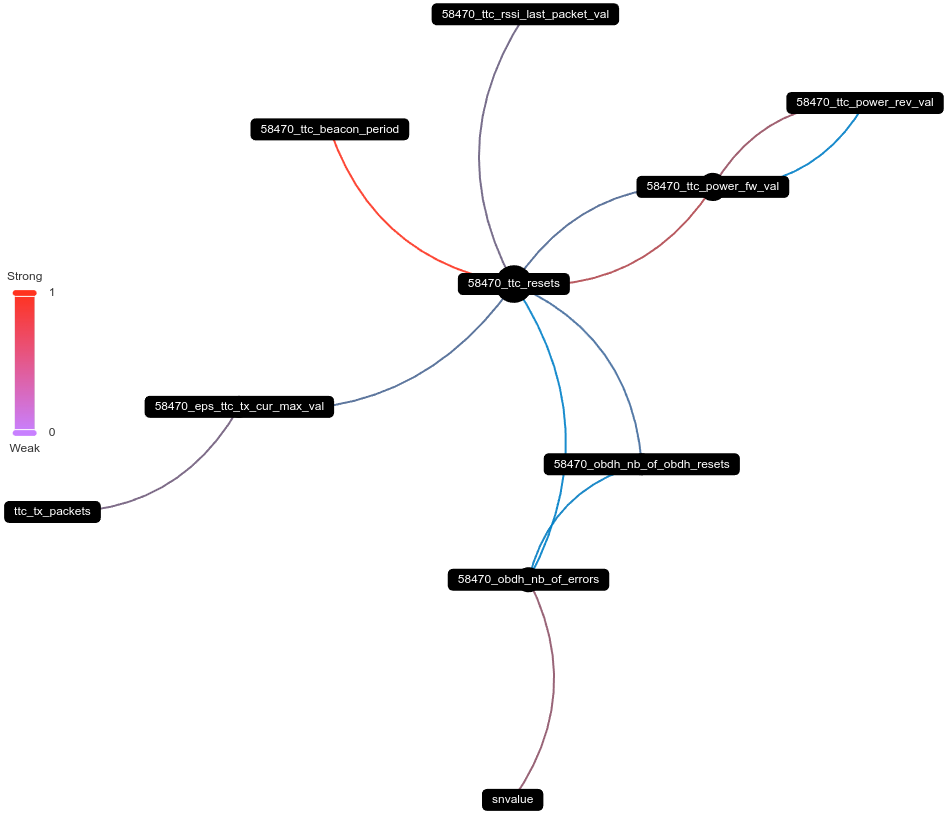
\includegraphics[width=0.95\textwidth]{sat/enso_sunspot.png}
	\caption{Граф кросс-корреляций по солнечным пятнам и инженерным параметрам (ENSO)}
	\label{fig:enso_sunspot}
\end{figure}

\begin{figure}[H]
	\centering
	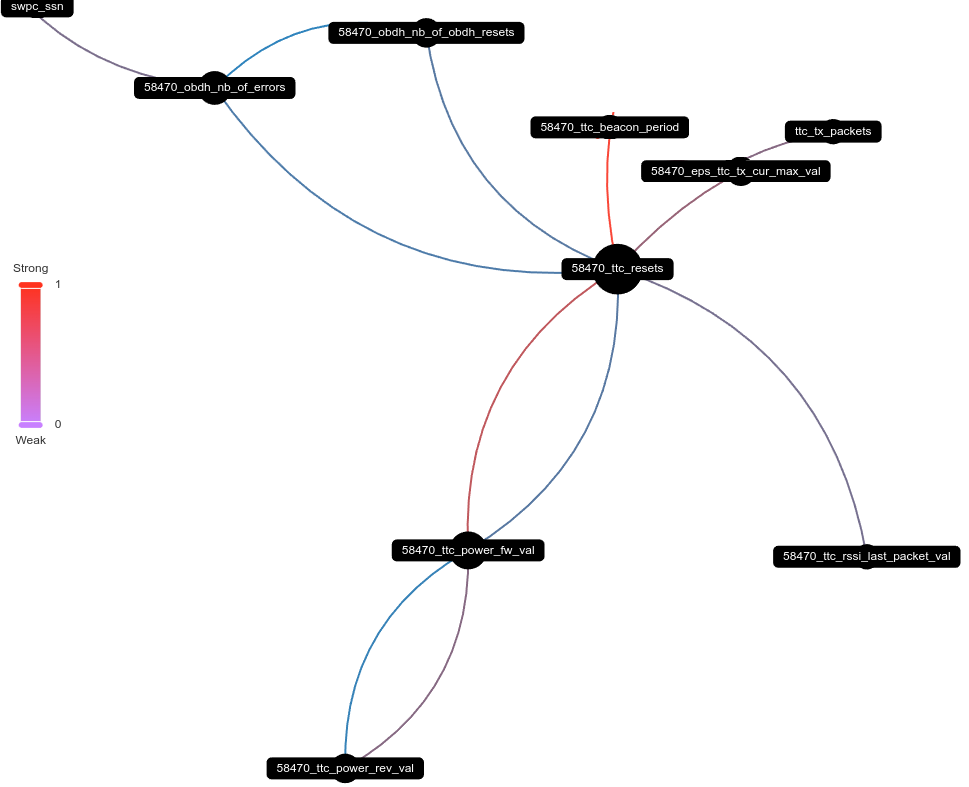
\includegraphics[width=0.95\textwidth]{sat/enso_ssn.png}
	\caption{Граф кросс-корреляций по числу солнечных пятен (ENSO)}
	\label{fig:enso_ssn}
\end{figure}

\begin{figure}[H]
	\centering
	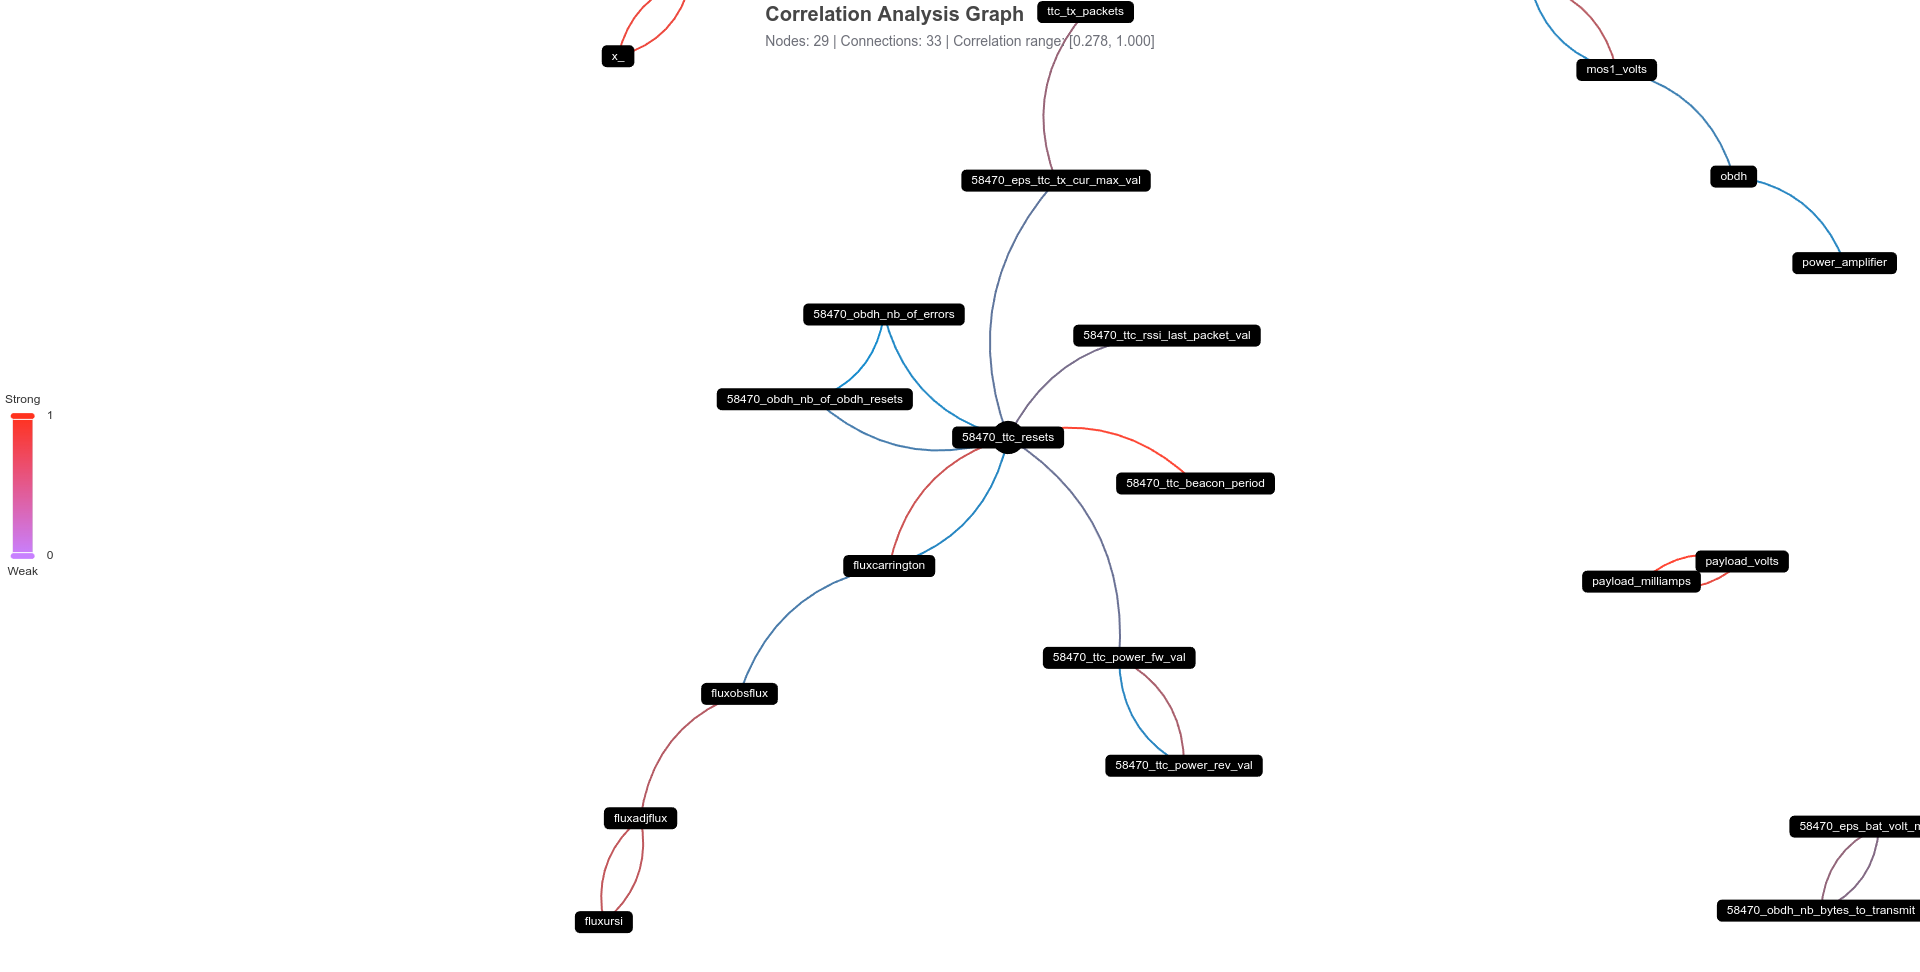
\includegraphics[width=0.95\textwidth]{sat/enso_flux.png}
	\caption{Граф кросс-корреляций по солнечному радиоизлучению (ENSO)}
	\label{fig:enso_flux}
\end{figure}

В центре большинства графов находится параметр \texttt{58470\_ttc\_resets} -
число перезапусков радиотехнического комплекса передачи данных. Этот параметр
тесно связан с ошибками и сбоями в подсистемах передачи и обработки информации
(\texttt{58470\_obdh\_nb\_of\_errors},
\texttt{58470\_obdh\_nb\_of\_obdh\_resets}), а также с энергетическими
характеристиками (\texttt{58470\_eps\_ttc\_bx\_cur\_max\_val},
\texttt{58470\_ttc\_power\_fw\_val}, \texttt{58470\_ttc\_power\_rev\_val}).

Анализ графа на рисунке~\ref{fig:enso_sunspot} показывает, что увеличение
количества ошибок и перезапусков в подсистемах (\texttt{obdh}, \texttt{ttc})
коррелирует с изменениями энергетических параметров. Связи между
\texttt{ttc\_resets} и \texttt{beacon\_period}, а также между
\texttt{ttc\_resets} и \texttt{ttc\_power\_fw/rev\_val} имеют различную силу:
наиболее сильные (красные рёбра) соответствуют случаям, когда сбои в питании или
перегрузки приводят к аварийным перезапускам радиотракта. Слабые (синие) и
средние (фиолетовые) связи фиксируют менее выраженные, но устойчивые зависимости
- например, рост тока передачи (\texttt{eps\_ttc\_bx\_cur\_max\_val}) при
увеличении числа пакетов (\texttt{ttc\_tx\_packets}), что отражает
закономерности работы CubeSat на низкой околоземной
орбите~\cite{expleo_enso_pdf}.

На графе~\ref{fig:enso_ssn} прослеживается связь между числом солнечных пятен
(\texttt{swpc\_ssn}) и инженерными параметрами. В периоды роста солнечной
активности наблюдается тенденция к снижению числа ошибок и перезапусков, что
связано с увеличением выработки энергии солнечными панелями и стабилизацией
работы энергетической подсистемы. Однако, при экстремальных событиях возможен
обратный эффект - рост числа сбоев из-за повышения радиационного
фона~\cite{nasa_shielding}.

Граф~\ref{fig:enso_flux} демонстрирует аналогичные закономерности для параметров
солнечного радиоизлучения (\texttt{fluxcarrington}, \texttt{fluxobsflux},
\texttt{fluxadjflux}, \texttt{fluxursi}). Сильные корреляции между током
нагрузки полезной нагрузки (\texttt{payload\_milliamps}) и напряжением
(\texttt{payload\_volts}) указывают на прямую зависимость между уровнем
солнечного излучения и энергетическими возможностями спутника. Связи между
параметрами питания и сбоями подтверждают, что энергетические провалы или
перегрузки приводят к увеличению числа перезапусков и ошибок в системах передачи
и обработки данных.

В периоды низкой солнечной активности возможно снижение напряжения и тока на
батареях (\texttt{eps\_bat\_volt\_avg\_val}, \texttt{battery\_voltage\_volts}),
что увеличивает риск сбоев и аварийных перезапусков. Это типично для малых
CubeSat, построенных на коммерческих компонентах без специализированной
радиационной защиты~\cite{expleo_enso_pdf, nanosats_enso}.

Таким образом, анализ графов кросс-корреляций для ENSO показывает, что ключевым
фактором надёжности работы спутника является энергетическая стабильность,
напрямую зависящая от солнечной активности. В периоды благоприятных условий
(высокая активность, стабильный поток излучения) количество сбоев и ошибок
минимально, а при экстремальных событиях или энергетическом дефиците -
возрастает.


\section{Структурный анализ графов кросс-корреляций и особенностей спутника Veronika}

\subsection{Структурные и технологические особенности спутника Veronika}

Veronika - это 1U CubeSat, разработанный и произведённый словацкой компанией Spacemanic при поддержке Deutsche Schule Bratislava, PLANETUM (Прага) и Технического университета Кошице~\cite{spacemanic_veronika, nanosats_veronika, satnogs_veronika, kozmonautika_veronika}. Аппарат был выведен на солнечно-синхронную орбиту высотой 550 км 11 ноября 2023 года ракетой Falcon 9 (миссия Transporter-9). Масса спутника составляет 1010 г, размеры - стандартный 1U форм-фактор.

Конструкция Veronika выполнена с использованием проверенных компонентов с богатой летной историей, разработанных и интегрированных компанией Spacemanic~\cite{spacemanic_veronika, nanosats_veronika}. Корпус изготовлен из анодированного алюминиевого сплава, что обеспечивает необходимую механическую прочность и минимальный уровень дегазации. Для электроизоляции и защиты от температурных перепадов применяются полиимидные материалы (например, Kapton), а для крепежа и кабельных соединений - стандартные полимерные материалы, используемые в индустрии малых спутников~\cite{spacemanic_veronika, kozmonautika_veronika}.

На борту установлены две камеры (uCAM и iCAM) для съёмки Земли, каждая из которых отличается компактностью, малой массой и низким энергопотреблением. uCAM - это малогабаритная камера с разрешением до 640×480, CMOS-сенсором и углом обзора 116°, а iCAM - более лёгкая камера с VGA-разрешением и углом обзора 60°~\cite{kozmonautika_veronika}.

Энергетическая подсистема включает солнечные панели и аккумуляторную батарею, обеспечивающие питание всех систем CubeSat. Радиокомплекс поддерживает работу в любительских диапазонах UHF (436.680 МГц) и VHF (145.925 МГц), реализованы протоколы AX.25, GFSK и CW для передачи телеметрии и пользовательских сообщений~\cite{spacemanic_veronika, nanosats_veronika, kozmonautika_veronika}. Важной особенностью является наличие экспериментальной системы ориентации (ADCS) с электромагнитными приводами и приёмником GNSS, что позволяет спутнику стабилизироваться и определять своё положение в пространстве~\cite{spacemanic_veronika, nanosats_veronika}.

Вся компонентная база - коммерческая (COTS), без применения специализированных радиационно-стойких решений, что типично для современных образовательных и технологических CubeSat~\cite{spacemanic_veronika, nanosats_veronika, nasa_soa}. Перед запуском Veronika прошла полный цикл испытаний на вибрацию, термовакуум и электромагнитную совместимость, что подтверждено инженерными отчётами компании~\cite{spacemanic_veronika, kozmonautika_veronika}.

\subsection{Анализ графов кросс-корреляций для спутника Veronika}

На рисунках~\ref{fig:veronika_sunspot}--\ref{fig:veronika_flux} представлены
графы кросс-корреляций между инженерными и внешними параметрами спутника
Veronika.

\begin{figure}[H]
	\centering
	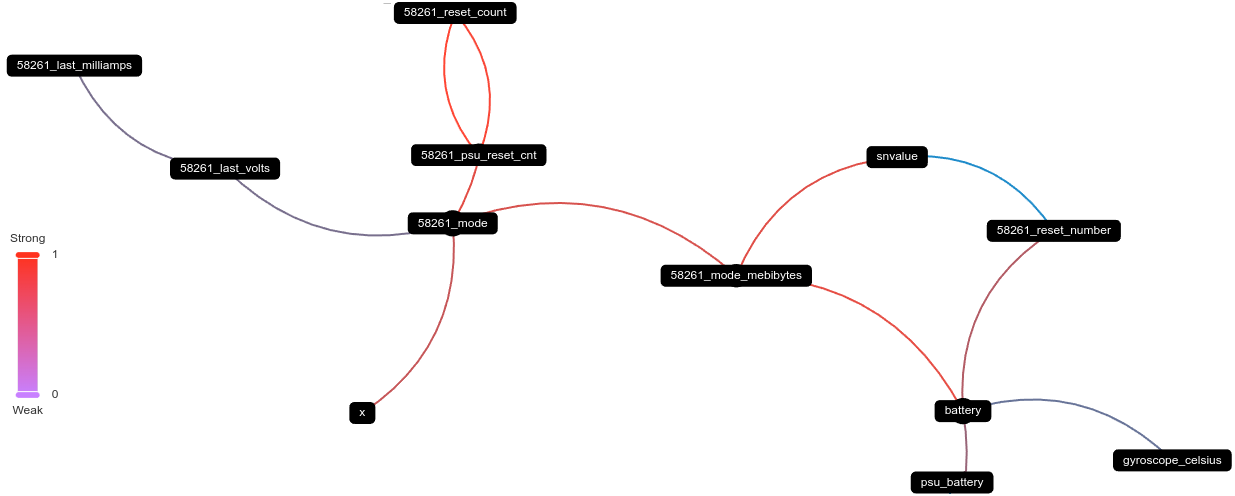
\includegraphics[width=0.95\textwidth]{sat/veronika_sunspot.png}
	\caption{Граф кросс-корреляций по инженерным параметрам и солнечным пятнам (Veronika)}
	\label{fig:veronika_sunspot}
\end{figure}

\begin{figure}[H]
	\centering
	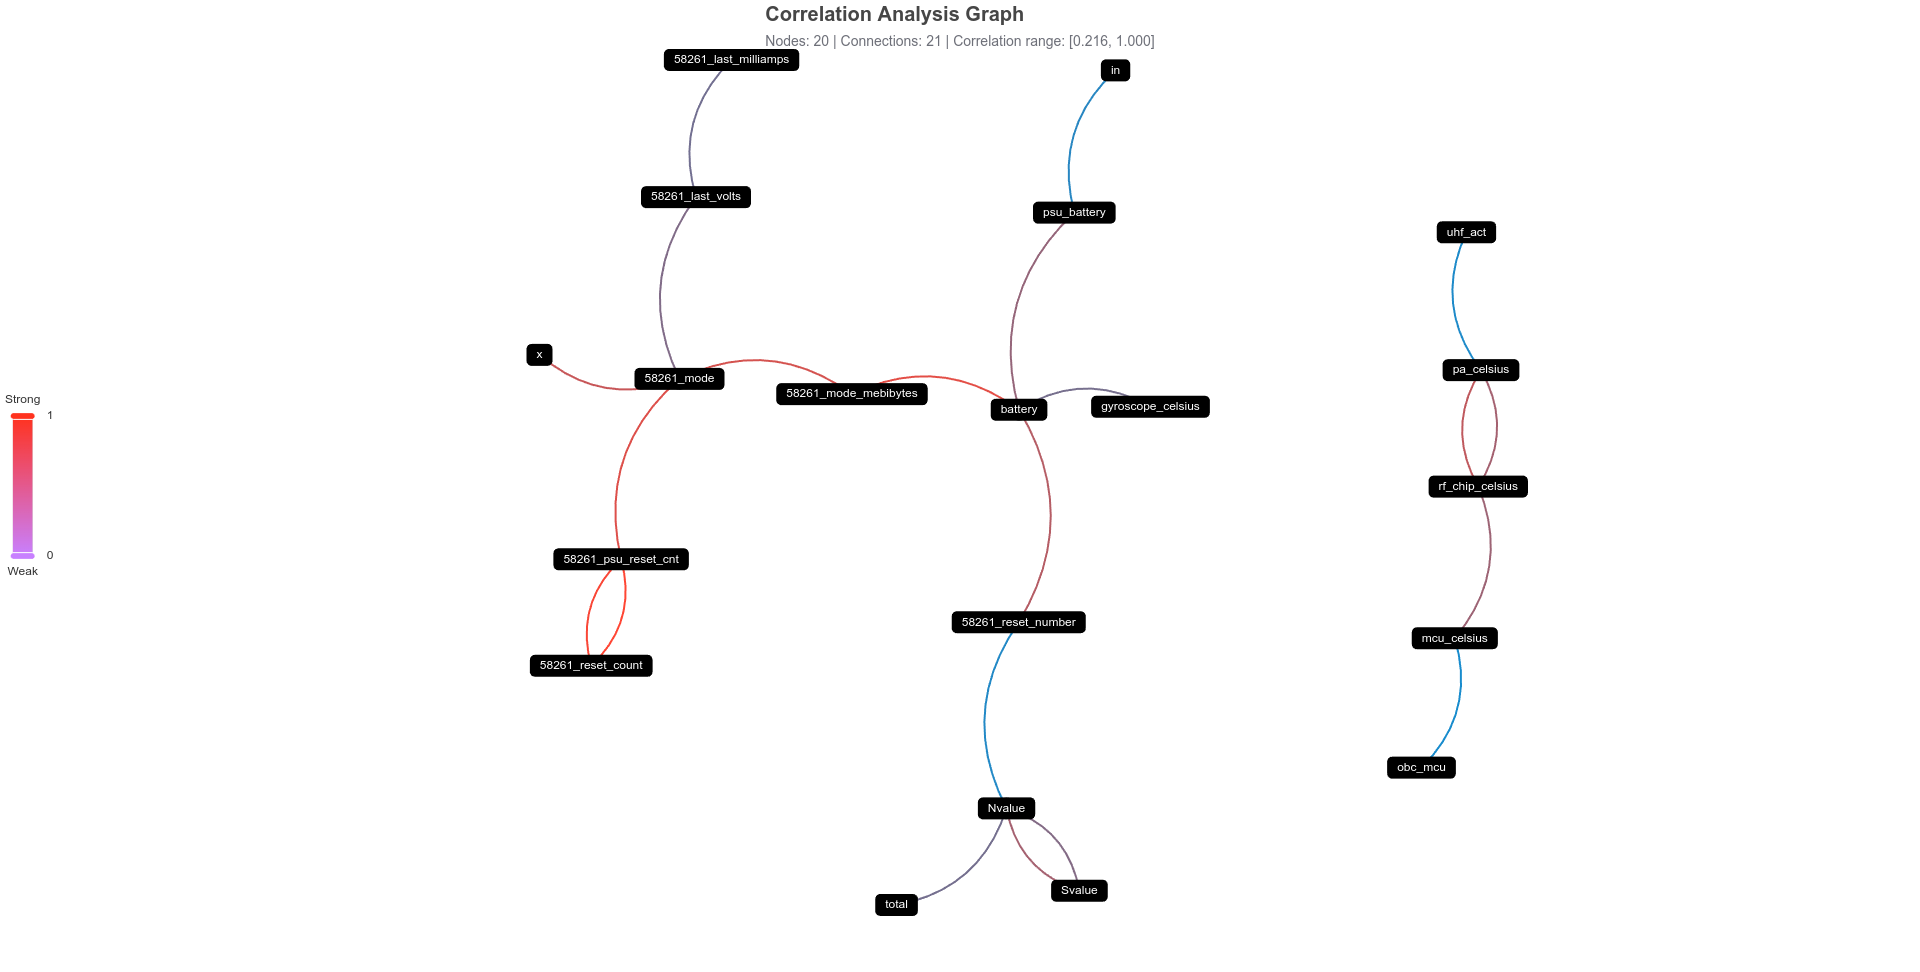
\includegraphics[width=0.95\textwidth]{sat/veronika_hemi.png}
	\caption{Граф кросс-корреляций по гемиcферическим числам солнечных пятен (Veronika)}
	\label{fig:veronika_hemi}
\end{figure}

\begin{figure}[H]
	\centering
	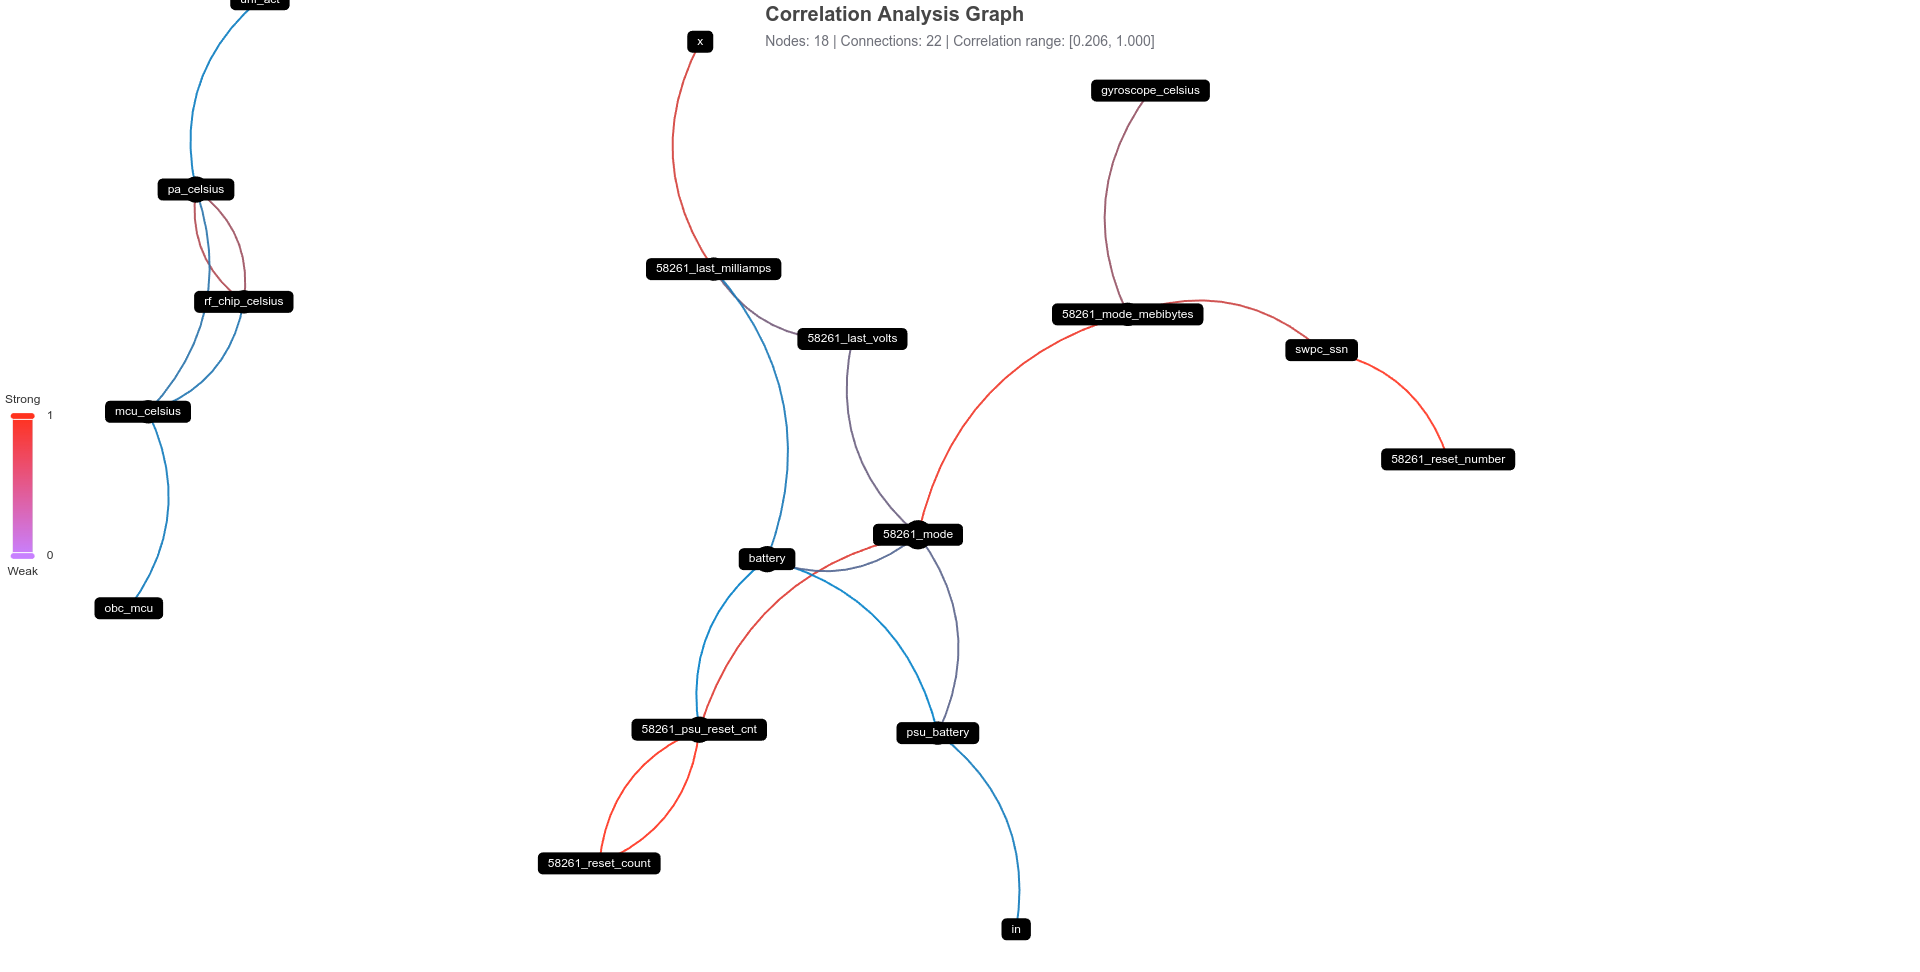
\includegraphics[width=0.95\textwidth]{sat/veronika_ssn.png}
	\caption{Граф кросс-корреляций по среднемесячному числу солнечных пятен (Veronika)}
	\label{fig:veronika_ssn}
\end{figure}

\begin{figure}[H]
	\centering
	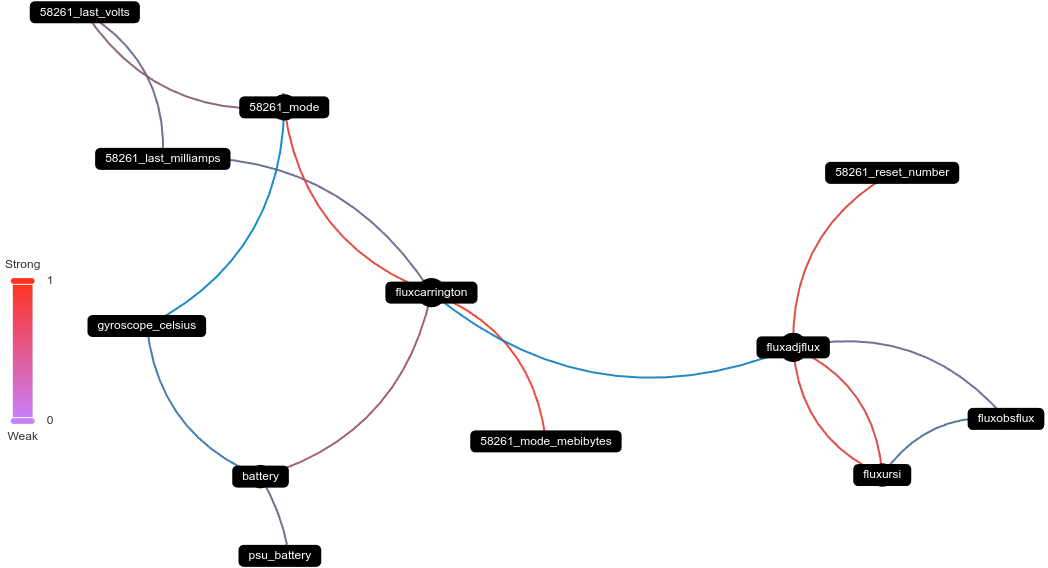
\includegraphics[width=0.95\textwidth]{sat/veronika_flux.png}
	\caption{Граф кросс-корреляций по солнечному радиоизлучению (Veronika)}
	\label{fig:veronika_flux}
\end{figure}


В центре представленных графов кросс-корреляций для спутника Veronika (рис.~\ref{fig:veronika_sunspot}--\ref{fig:veronika_flux}) находятся параметры, связанные не только с энергетикой, но и с логикой функционирования, сбоями и тепловыми режимами ключевых подсистем. Наиболее сильные корреляции (красные рёбра) фиксируются между счетчиками перезапусков (\texttt{58261\_reset\_count}, \texttt{58261\_psu\_reset\_cnt}, \texttt{58261\_reset\_number}) и рабочими режимами (\texttt{58261\_mode}, \texttt{58261\_mode\_mebbytes}), что указывает на прямую зависимость надёжности работы от переходов между режимами и состояния управляющей электроники. Это типично для малых спутников с ограниченными ресурсами: сбои часто инициируются не только энергетическими провалами, но и логическими ошибками, накоплением ошибок памяти или перегревом микроконтроллеров~\cite{spacemanic_veronika, nanosats_veronika}.

Графы демонстрируют, что влияние солнечной активности на Veronika не является однозначно положительным. С одной стороны, рост солнечной активности (параметры \texttt{swpc\_ssn}, \texttt{fluxcarrington}, \texttt{fluxobsflux}, \texttt{fluxadjflux}, \texttt{fluxursi}) приводит к увеличению выработки энергии солнечными панелями, что проявляется в корреляциях между током нагрузки (\texttt{58261\_last\_milliamps}), напряжением (\texttt{58261\_last\_volts}, \texttt{battery}, \texttt{psu\_battery}) и снижением числа аварийных перезапусков~\cite{spacemanic_veronika, nanosats_veronika}. Однако при экстремальных вспышках и магнитных бурях наблюдается усиление негативных эффектов: возрастает количество сбоев, увеличивается число аппаратных перезапусков, фиксируются скачки температур в чувствительных узлах (кластер температурных параметров: \texttt{mcu\_celsius}, \texttt{rf\_chip\_celsius}, \texttt{pa\_celsius}, \texttt{uhf\_act}, \texttt{obc\_mcu})~\cite{nasa_soa, stehlikova_veronika}.

Особо стоит отметить, что корреляции между температурными параметрами и сбоями не всегда линейны: перегрев радиотракта или управляющего микроконтроллера (\texttt{mcu\_celsius}, \texttt{rf\_chip\_celsius}) может быть как следствием интенсивной работы в условиях высокой солнечной активности, так и результатом внутренних сбоев, вызванных, например, ошибками в логике управления питанием. В ряде случаев наблюдается каскадный эффект: рост солнечной активности $\rightarrow$ увеличение выработки энергии $\rightarrow$ рост нагрузки на радиотракт $\rightarrow$ рост температуры $\rightarrow$ увеличение вероятности аппаратных сбоев и перезапусков~\cite{stehlikova_veronika, spacemanic_veronika}.

Связи между параметрами \texttt{battery}, \texttt{psu\_battery}, \texttt{last\_milliamps}, \texttt{last\_volts} и внешними индексами солнечной активности подтверждают, что энергетическая стабильность - лишь один из факторов надёжности. При недостатке солнечной энергии (низкая активность или затенение орбиты) риск сбоев увеличивается из-за разрядки батарей, однако при избыточной активности возможны перегревы и повреждения электроники, особенно в отсутствие специализированной радиационной и тепловой защиты, как у Veronika~\cite{spacemanic_veronika, stehlikova_veronika}.








\begin{conclusion}
\titleformat{\section}[block]{\large\bfseries\filcenter}{}{0em}{}
\chapter*{Заключение}

В рамках данной работы было проведено комплексное исследование влияния солнечной
активности на функционирование малых космических аппаратов с использованием
методов машинного обучения и анализа графов кросс-корреляций. Основные
результаты исследования можно сформулировать следующим образом.

Разработана и реализована усовершенствованная методика анализа взаимосвязей
между параметрами солнечной активности и электротехническими характеристиками
космических аппаратов на базе платформы Polaris ML. Ключевые улучшения включают:

\begin{enumerate}
	\item Модификацию базового алгоритма XGBoost с учетом специфики спутниковых данных, включая оптимизацию функции потерь, введение временных признаков второго порядка и реализацию каскадного подхода с поэтапным уточнением предсказаний.

	\item Расширение возможностей конфигурирования модели путем увеличения числа оптимизируемых гиперпараметров до 30, что позволило повысить точность модели с F1-Score 0.87 (Random Forest) до 0.94 (модифицированный XGBoost) при одновременном снижении времени обучения с 45 до 27 минут.

	\item Внедрение параллельных вычислений, обеспечивших ускорение обработки данных в 25 раз (с 180 до 7 секунд) для временных рядов объемом до 5 лет при использовании 24 вычислительных потоков.

	\item Интеграцию MLflow для стандартизации ведения отчетности и управления экспериментами, что значительно упростило сравнительный анализ моделей с разными гиперпараметрами ценой незначительного снижения производительности (увеличение времени обработки с 7 до 10 секунд).
\end{enumerate}

Проведенный структурный анализ графов кросс-корреляций для спутников GRIFEX,
ENSO, Veronika, LASARsat и INSPIRESat-1 выявил как общие закономерности, так и
специфические особенности их взаимодействия с солнечной активностью:

\begin{enumerate}
	\item Для спутника GRIFEX, оснащенного радиационно-стойкими материалами, высокая солнечная активность преимущественно оказывает положительное влияние на функционирование систем за счет увеличения энергетических возможностей при сохранении устойчивости к ионизирующему излучению.

	\item Для спутников с использованием коммерческих компонентов (ENSO, Veronika, LASARsat) характерна более сложная нелинейная структура взаимосвязей: умеренное увеличение солнечной активности стабилизирует работу, в то время как экстремальные события провоцируют каскадные сбои. При этом для Veronika наблюдается особая чувствительность к тепловым режимам, а для LASARsat критически важна стабильность ориентации в пространстве, поскольку его основная миссия по тестированию лазерного воздействия требует точного позиционирования относительно наземных лазерных установок.

	\item INSPIRESat-1, благодаря более сложной системе терморегуляции и увеличенным габаритам (9U CubeSat), демонстрирует промежуточную устойчивость к внешним воздействиям. Анализ графов выявил сильную связь между режимами работы научной аппаратуры (DAXSS) и солнечным вектором, указывающую на адаптивность управления в зависимости от внешних условий.
\end{enumerate}

Полученные результаты имеют как теоретическую, так и практическую значимость. С
теоретической точки зрения, предложен математически обоснованный подход к
параллельному вычислению кросс-корреляций между временными рядами, что вносит
вклад в развитие методов анализа больших данных в космической отрасли. С
практической стороны, созданная система позволяет существенно сократить время
обработки телеметрии малых космических аппаратов и выявлять нетривиальные
взаимосвязи между солнечной активностью и функционированием бортовых систем.

Дальнейшее развитие работы возможно в направлении интеграции асинхронного
логирования в MLflow для минимизации влияния на производительность, расширения
набора анализируемых спутников для обеспечения статистической значимости, а
также совершенствования модели оптимизации гиперпараметров с применением
байесовских методов вместо сеточного поиска.

\end{conclusion}

% === БИБЛИОГРАФИЯ === %
\newpage

\printbibliography[heading=bibintoc,title={Список использованной литературы},env=paragraphbib]

% === ПРИЛОЖЕНИЯ === %
\newpage
\appendix

\begin{attachements}
\renewcommand{\chaptermark}[1]{\markboth{}{}}
\renewcommand{\sectionmark}[1]{\markright{\arabic{section}.\ #1}}

% Fix for malformed section formatting
\titleformat{\section}[block]{\large\bfseries\filcenter}{}{0em}{}
\chapter*{Приложения}

\section{Приложение \arabic{section}}
\label{subsec:old_polaris_learn_config}

В данном приложении представлена старая конфигурация, используемая для формирования нейронного ансамбля с помощью алгоритма XGBoost.

%\lstinputlisting[language=Java, label={lst:old_polaris_config}, caption=Конфигурация XGBoost]{../code/old_polaris_cfg.json}

\section{Приложение \arabic{section}}
\label{subsec:attachement_cubesat_design}

\begin{sidewaysfigure}[htbp]
    \centering
    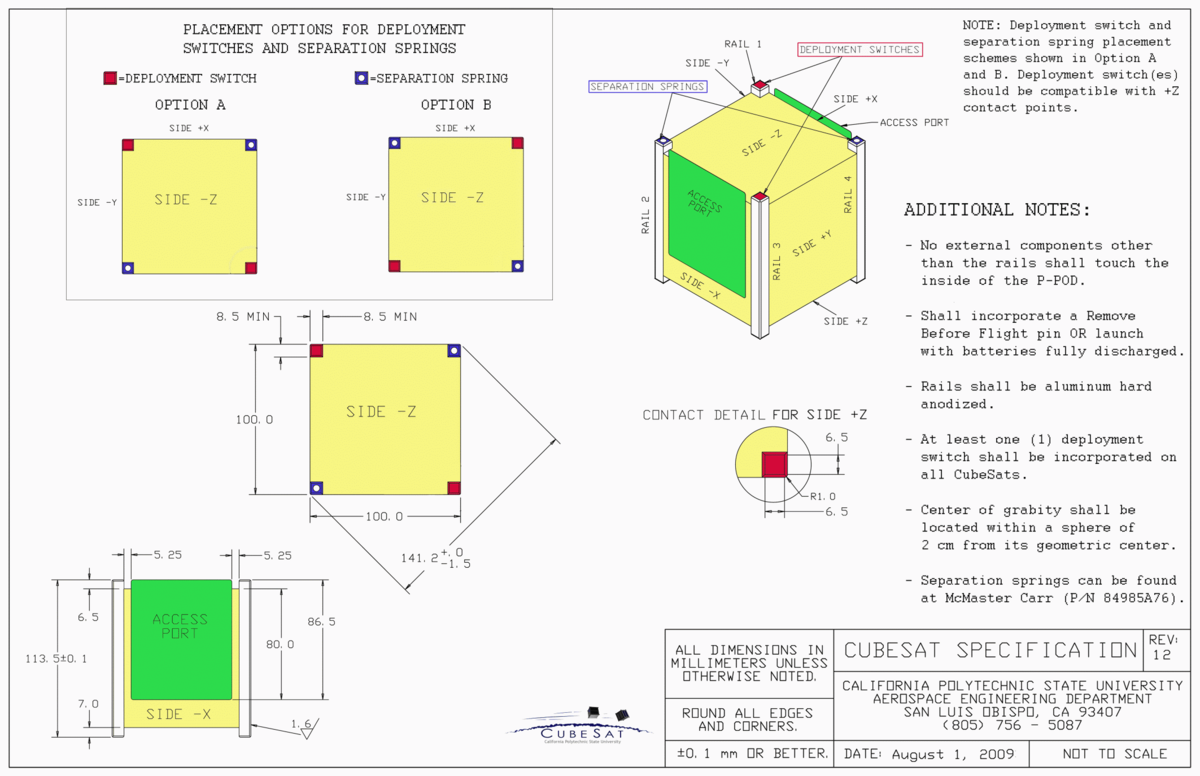
\includegraphics[width=1.0\linewidth]{img/cubesat_design.png}
    \caption{Спецификация блока спутника типа CubeSat}
\end{sidewaysfigure}





\end{attachements}

\end{document}